\subsection{Overview}
The following diagram represents the high level architecture of the system, including the external entities that will interact with it.\\
\begin{figure}[H]
    \centering
    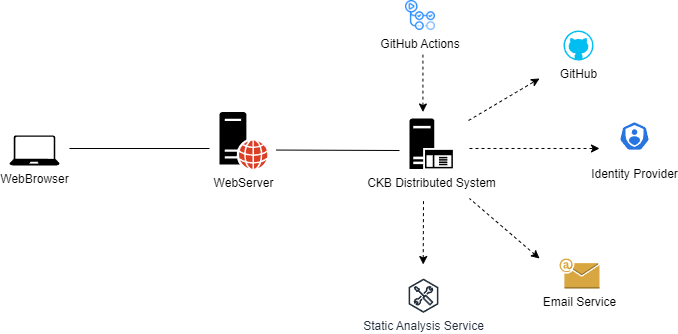
\includegraphics[width=1\textwidth]{Diagrams/overview.png}
    \caption{CKB system diagram}
    \label{overview_diagram}
\end{figure}
The main elements contained in Figure \ref{overview_diagram} are:
\begin{itemize}
    \item \textbf{WebBrowser} used by students and educators to access the system functionalities through the web application.
    \item \textbf{WebServer} whose functions are:
    \begin{itemize}
        \item Serving static assets (HTML, CSS, JavaScript) to the client, necessary for handling the initial rendering of the UI.
        \item Managing the client-side application and routing.
        \item Generating requests directed to the backend system.
    \end{itemize}
    \item \textbf{CKB Distributed System} which is the distributed system composed of multiple microservices that implement the core functionalities of the system. Its in charge of the data management, application and integration logic of the whole CKB platform.
    \item \textbf{External Entities} the CKB Distributed System must be able to integrate with to accomplish its functionalities. The arrow in the diagram highlights the direction of the interaction between the system and the external entities.
\end{itemize}

\subsection{Component view}
The following component diagram highlights the main components of the system and their interaction with external entities and services. In the diagram, the components have been organized to highlight the logical grouping of the system elements.

The WebApplication component represents the presentation layer of the system, being the only entry point for the users. The application and integration logics are represented together due to their tight interaction, while the data layer contains the databases accessed by the respective microservices.

Different colors are used to highlight components that share similar roles in the system.
\begin{itemize}
    \item \textcolor{orange}{Orange} components represent the system's microservices. Complex microservices have been further decomposed into subcomponents, for a more fine grained representation. Some microservices have an important role in the integration and communication with external entities as well, but have been depicted with their orange color used for microservices. This aspect will be clarified in the detailed description of the components that follows the diagram.
    \item \textcolor{myyellow}{Yellow} components represent the model of the database accessed by its microservice. The model offers to the microservice an abstraction of the database, allowing it to access the data without knowing the underlying database implementation technology.
    \item \textcolor{violet}{Violet} has been used to highlight components or services that cover an important role for the communication between microservices. It has been used for the queues subcomponents, which are used to implement the asynchronous and concurrent communication between specific microservices. Also the ServiceRegistry has been represented with the this color, since it enables the communication in the system. It's important to notice that for the sake of simplicity and readability, the interface offered by the ServiceRegistry has been depicted with some dotted arrows that connect all the microservices to it.
    \item \textcolor{red}{Red} components represent the external services that interact with the system.
    \item Finally, the \textcolor{mygreen}{green} color has been used to highlight the databases components that are used to store the data of the system.
\end{itemize}

\newpage
\thispagestyle{noheader}
\begin{figure}[H]
    \centering
    \vspace{-3.5cm}
    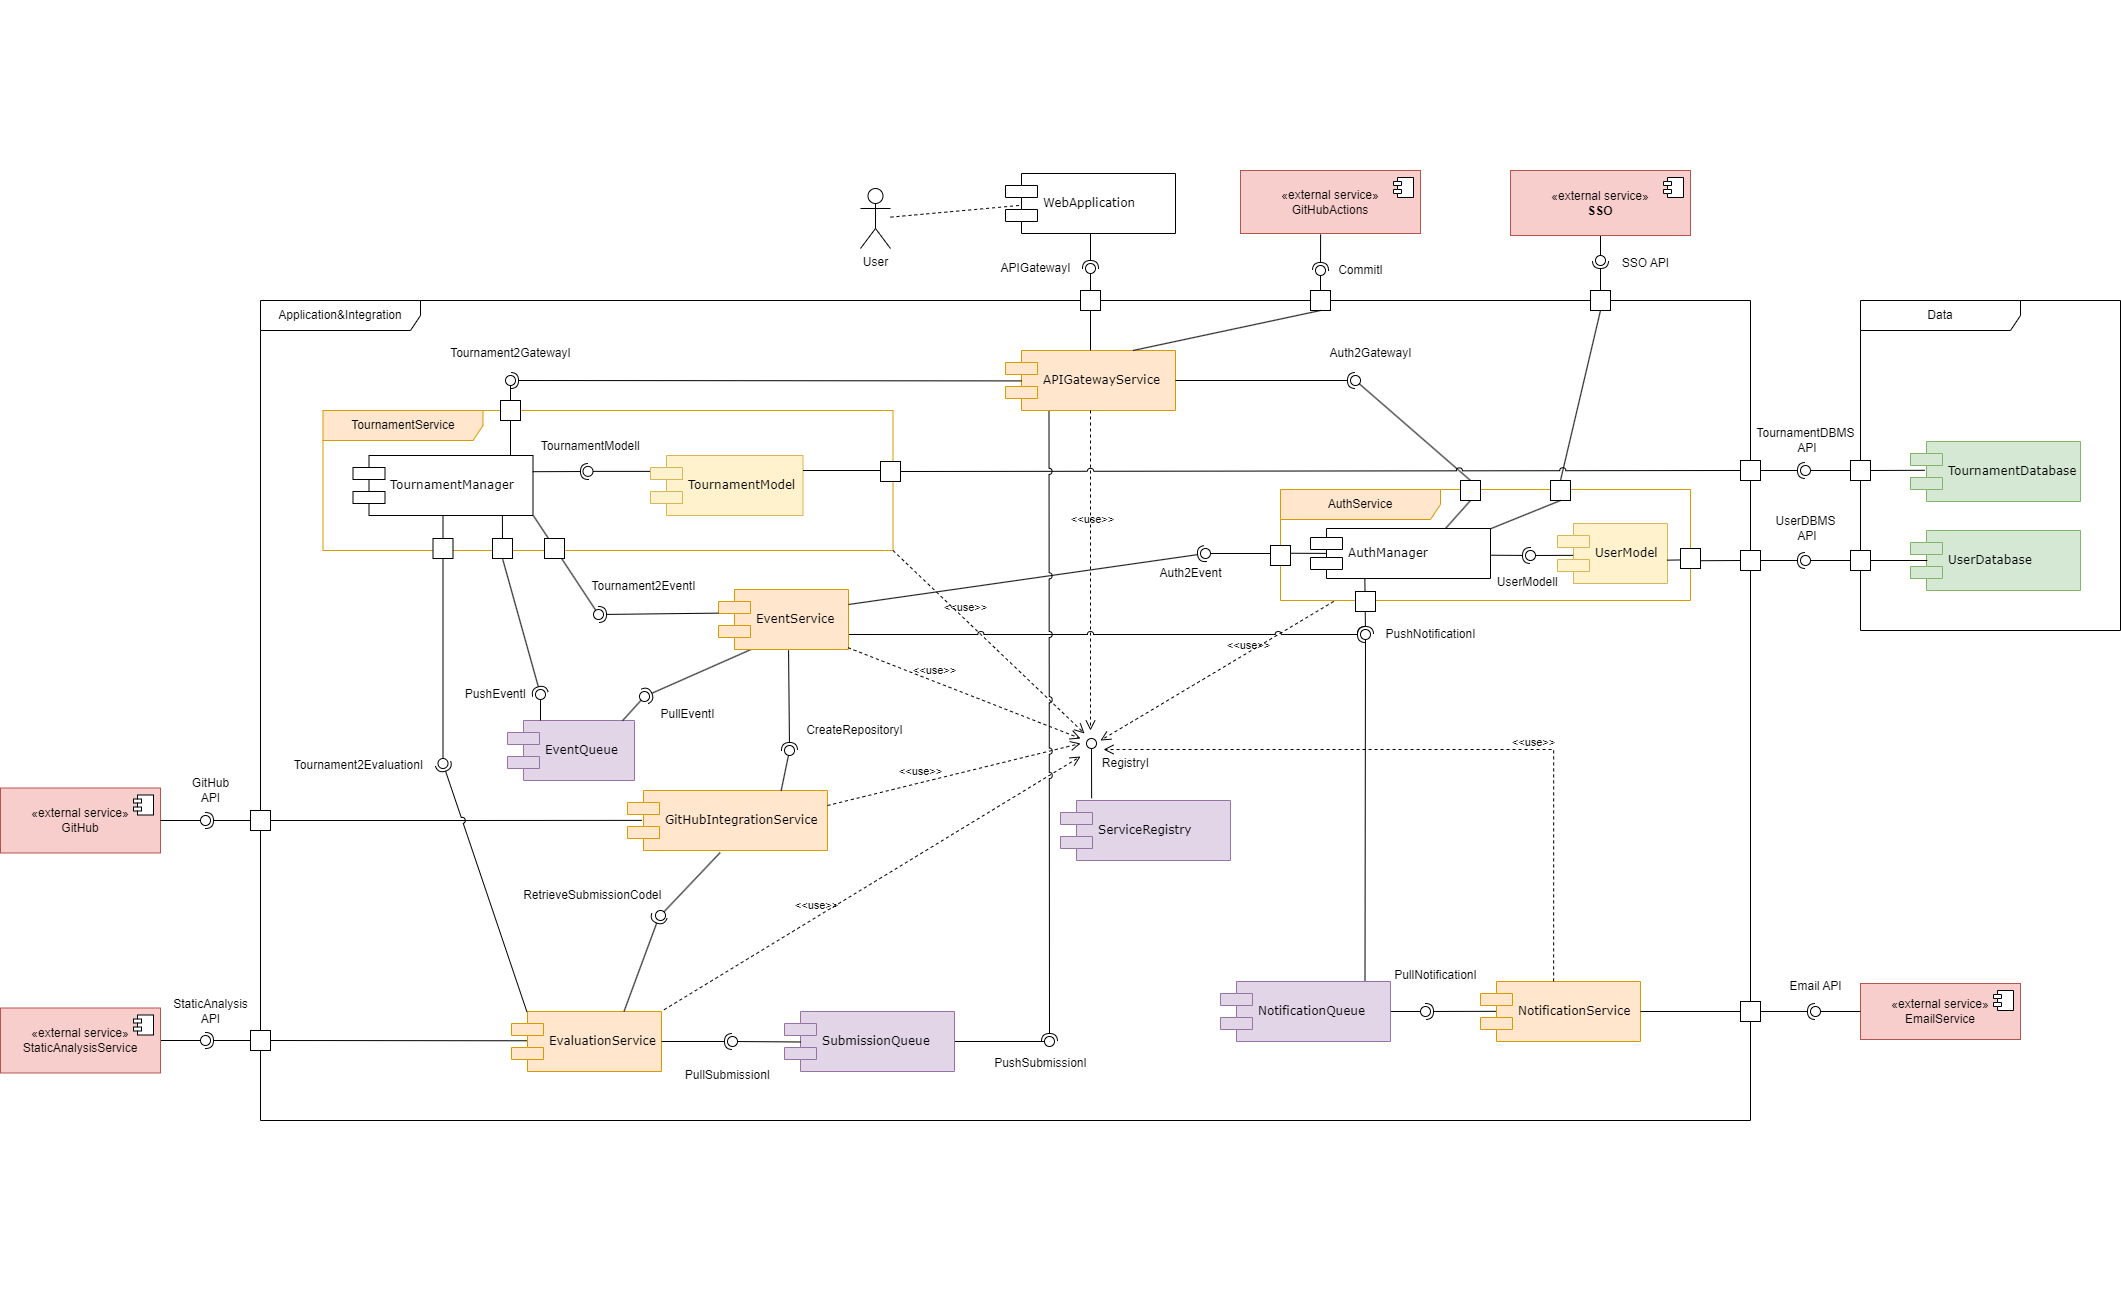
\includegraphics[width=1.6\textwidth,angle=90,origin=c]{Diagrams/component_diagram.png}
    \caption{Component diagram}
    \label{component_diagram}
\end{figure}

The components in Figure \ref{component_diagram} are :
\begin{itemize}
    \item \textbf{WebApplication}: the web app to which users of the CKB platform (students and educators) connect through a modern web browser. It is the front end of the system, and thanks to the interface offered by the \textbf{APIGatewayService}, allows users to manage and access the most important aspects of tournaments and battles.
    \item \textbf{APIGatewayService}: this component is the microservice that exposes the REST API used by the WebApplication. Indeed, it allows the implementation of the main functionalities needed by the users of the web application by orchestrating the microservices. It also offers a REST API, used by the GitHub Actions Service, to notify a submission of a student on the Github repository.
    It's also responsible for the following functionalities:
    \begin{itemize}
        \item Acts as a single entry point for client requests.
        \item Handles authentication, authorization through the interaction with the AuthService.
        \item Routes requests to the appropriate microservices that provide the required business functionality.
        \item Aggregates responses from multiple microservices if needed.
        \item Load balancing and API rate limiting.
    \end{itemize}
    \item \textbf{AuthService}: this component is the microservice that handles the authentication of the users of the system. To accomplish this task, it may be required to interact with external identity providers, depending on the user preferences. 
    It is responsible also for all the data related to the users of the system, such as their personal information and their roles. It includes the following subcomponents:
    \begin{itemize}
        \item \textbf{AuthManager}: implements the main logical functionalities of the AuthService, exposing APIs used by other microservices to authenticate and to retrieve user information.
        \item \textbf{UserModel}: represents the model of the database used by the AuthService to store the data related to the users of the system.
    \end{itemize}
    \item \textbf{TournamentService}: this component is the microservice that implements most of the functionalities needed by the users. It handles:
    \begin{itemize}
        \item Management of tournaments and battles: it allows the creation of battle and tournaments, enrollment of students to tournaments and battles.
        \item Management of events regarding tournaments and battles.
        \item Management of the ranking of the students.
        \item Management of data related to tournaments, battles and submissions
        \item Manual evaluation of the submissions of the students.
    \end{itemize}
    It is composed of the following subcomponents:
    \begin{itemize}
        \item \textbf{TournamentManager}: implements the main logical functionalities of the TournamentService, exposing APIs used by other microservices to manage tournaments, battles, team and their data.
        \item \textbf{TournamentModel}: represents the model of the database used by the TournamentService to store the data related to tournaments and battles.
    \end{itemize}
    \item \textbf{EventService}: periodically checks the EventQueue for events and processes them once the deadlines are reached. It is the consumer of events created by the TournamentService.
    \item \textbf{GitHubIntegrationService}: this component is the microservice that handles the integration with GitHub. It is responsible for the following functionalities:
    \begin{itemize}
        \item Creation of the GitHub repository of the battle.
        \item Retrieval of the code of the submission from the GitHub repository.
    \end{itemize}
    \item \textbf{EvaluationService}: this component is the microservice that handles the evaluation of the submissions of the students. It periodically checks the SubmissionQueue for submissions to evaluate and processing them, so it is the consumer of the events appended by the APIGatewayService on behalf of the GitHubActions.
     The submission notification contains only the token associated to the team (which corresponds to the teamId), so the service retrieves the code from the GitHub repository, interacting with the GitHubIntegrationService.
     This service is responsible for the following functionalities:
    \begin{itemize}
        \item Evaluation of the submissions, in terms of timeliness and functional analysis 
        \item Integration with external static code analysis tools to evaluate the quality of the code of the submissions.
    \end{itemize}
    \item \textbf{NotificationService}: this component is the microservice that handles the notifications of the users of the system. It periodically checks the NotificationQueue for new notifications to send and processing them. To perform this task, the NotificationService interacts with the external email service provider to send notifications to the users.
     It is responsible for the following functionalities:
    \begin{itemize}
        \item Dispatch of confirmation email to new registered users.
        \item Dispatch of email notifications to users in case of events related to tournaments and battles.
    \end{itemize}
    \item \textbf{ServiceRegistry}: this component handles the registration of the microservices to the system. It offers to all the microservices the following:
    \begin{itemize}
        \item Registration of the microservices istances to the system.
        \item Discovery of the microservices istances by the other microservices.
        \item Availability check of the microservices istances, by receiving periodic heartbeats from them.
    \end{itemize}
    \item \textbf{TournamentDatabase}: this component is the database used by the system to store the data related to tournaments and battles, including also scores and ranks.
    \item \textbf{UserDatabase}: this component is the database used by the system to store the data related to the users of the system, such as kind of user, email and usernames.
    \item \textbf{NotificationQueue}: queue that stores new notifications to be dispatched.
    \item \textbf{SubmissionQueue}: queue that stores notifications about new pending submissions, appended by the GitHubActions through the REST API exposed by the APIGatewayService, yet to be evaluated.
    \item \textbf{EventQueue}: the queue used by the TournamentService to manage the events related to tournaments and battles. It is implemented as a priority queue, so that events are ordered by their deadlines.
\end{itemize}
The Figure \ref{component_diagram} contains also some external entities the system interacts with:
\begin{itemize}
    \item \textbf{GitHub}: used by the system to retrieve the code of GitHub repositories and to create new repositories.
    \item \textbf{GitHubActions}: configured by the students on their GitHub repository to automatically notify the system when a new submission is pushed to the repository.
    \item \textbf{StaticAnalysisService}: used by the system to evaluate the quality of the code of the submissions.
    \item \textbf{EmailService}: used by the system to send emails to the users of the system.
    \item \textbf{SSO}: used by the system to offer the users the possibility to signup and login with their preferred identity provider.
\end{itemize}

\newpage
\subsection{Deployment view}
The following diagrams represent the deployment architecture of the system, highlighting the physical nodes on which the system will be deployed and the communication channels between them.

Figure \ref{deployment_net_diagram} shows how the network infrastructure of the system is organized: a first firewall is used separate the system from the Internet, creating a DMZ which will contain all the services that must be accessible from outside the system (i.e. Web server and API gateway), while a second firewall is used to separate the DMZ from the internal network of the organization.\\
\begin{figure}[H]
    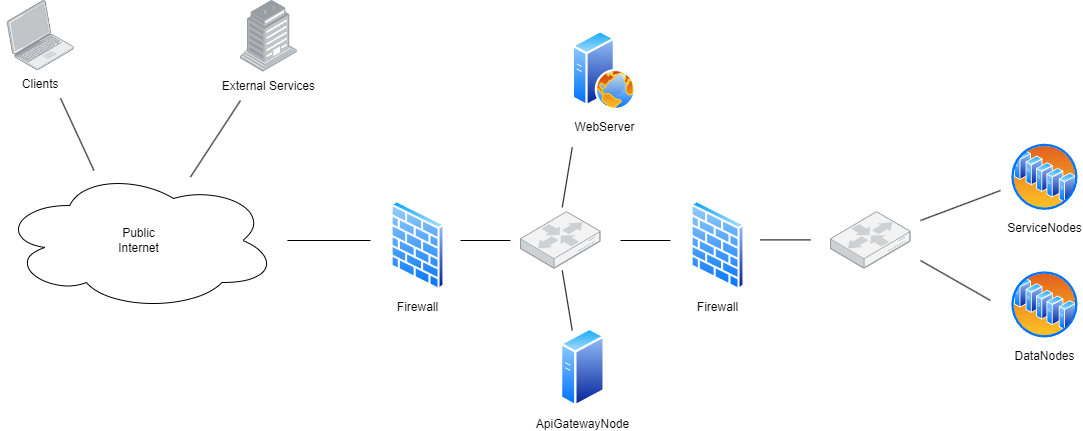
\includegraphics[width=1\textwidth]{Diagrams/deployment_network_diagram.png}
    \caption{Network perspective deployment diagram}
    \label{deployment_net_diagram}
\end{figure}

Figure \ref{deployment_diagram} instead represents how different software modules will be deployed on physical nodes. These nodes have been colored according to the color scheme defined in the component view section, with the only difference that the \textcolor{red}{red} color here has been used to identify the user's web browser and the \textcolor{myyellow}{yellow} one to represent the system's web server.\\ Important aspects that are worth noticing are:
\begin{itemize}
    \item Queues are deployed on a single phisical node. As we can see from the artifacts, all queues are built over the same code but replicated in a way that each type of microservice uses its own: this should increase modularity and maintainability of the system. Moreover these queues are logged (i.e. also persisted in secondary memory) so that, in case of failure, a new service can be deployed and the previous state of the queue can be restored: this allows the system to be fault tolerant by ensuring that no communication data is lost.
    \item Most of the architecture is deployed within Docker containers, providing a lightweight and scalable environment. Each instance of a microservice, instantiated as a separate container, follows a \textbf{thread-per-request model} to handle multiple incoming requests concurrently. This design choice optimizes resource utilization and responsiveness, allowing each microservice instance to efficiently manage concurrent requests through the creation of dedicated threads. The use of Docker ensures portability and consistency across different environments, enabling seamless deployment and scaling.\\ 
          The Service Registry instead is deployed in a non-containerized environment, since it is a critical component of the system and it is important to ensure its availability. In particular, in order to achieve this, a \textbf{master-slave schema} is used. The master instance is deployed on a different physical node with respect to other slave instances (only one in Figure \ref{deployment_diagram}): these have the task of monitoring the master instance and to copy its logs. In this way, if the master instance fails, one of the slave instances (e.g. chosen through a consensus algorithm) can be promoted to master so the system can continue to work from the point it left without any significant interruption.
\end{itemize}
\begin{figure}[H]
    \centering
    \vspace{-4cm}
    \hspace{1cm}
    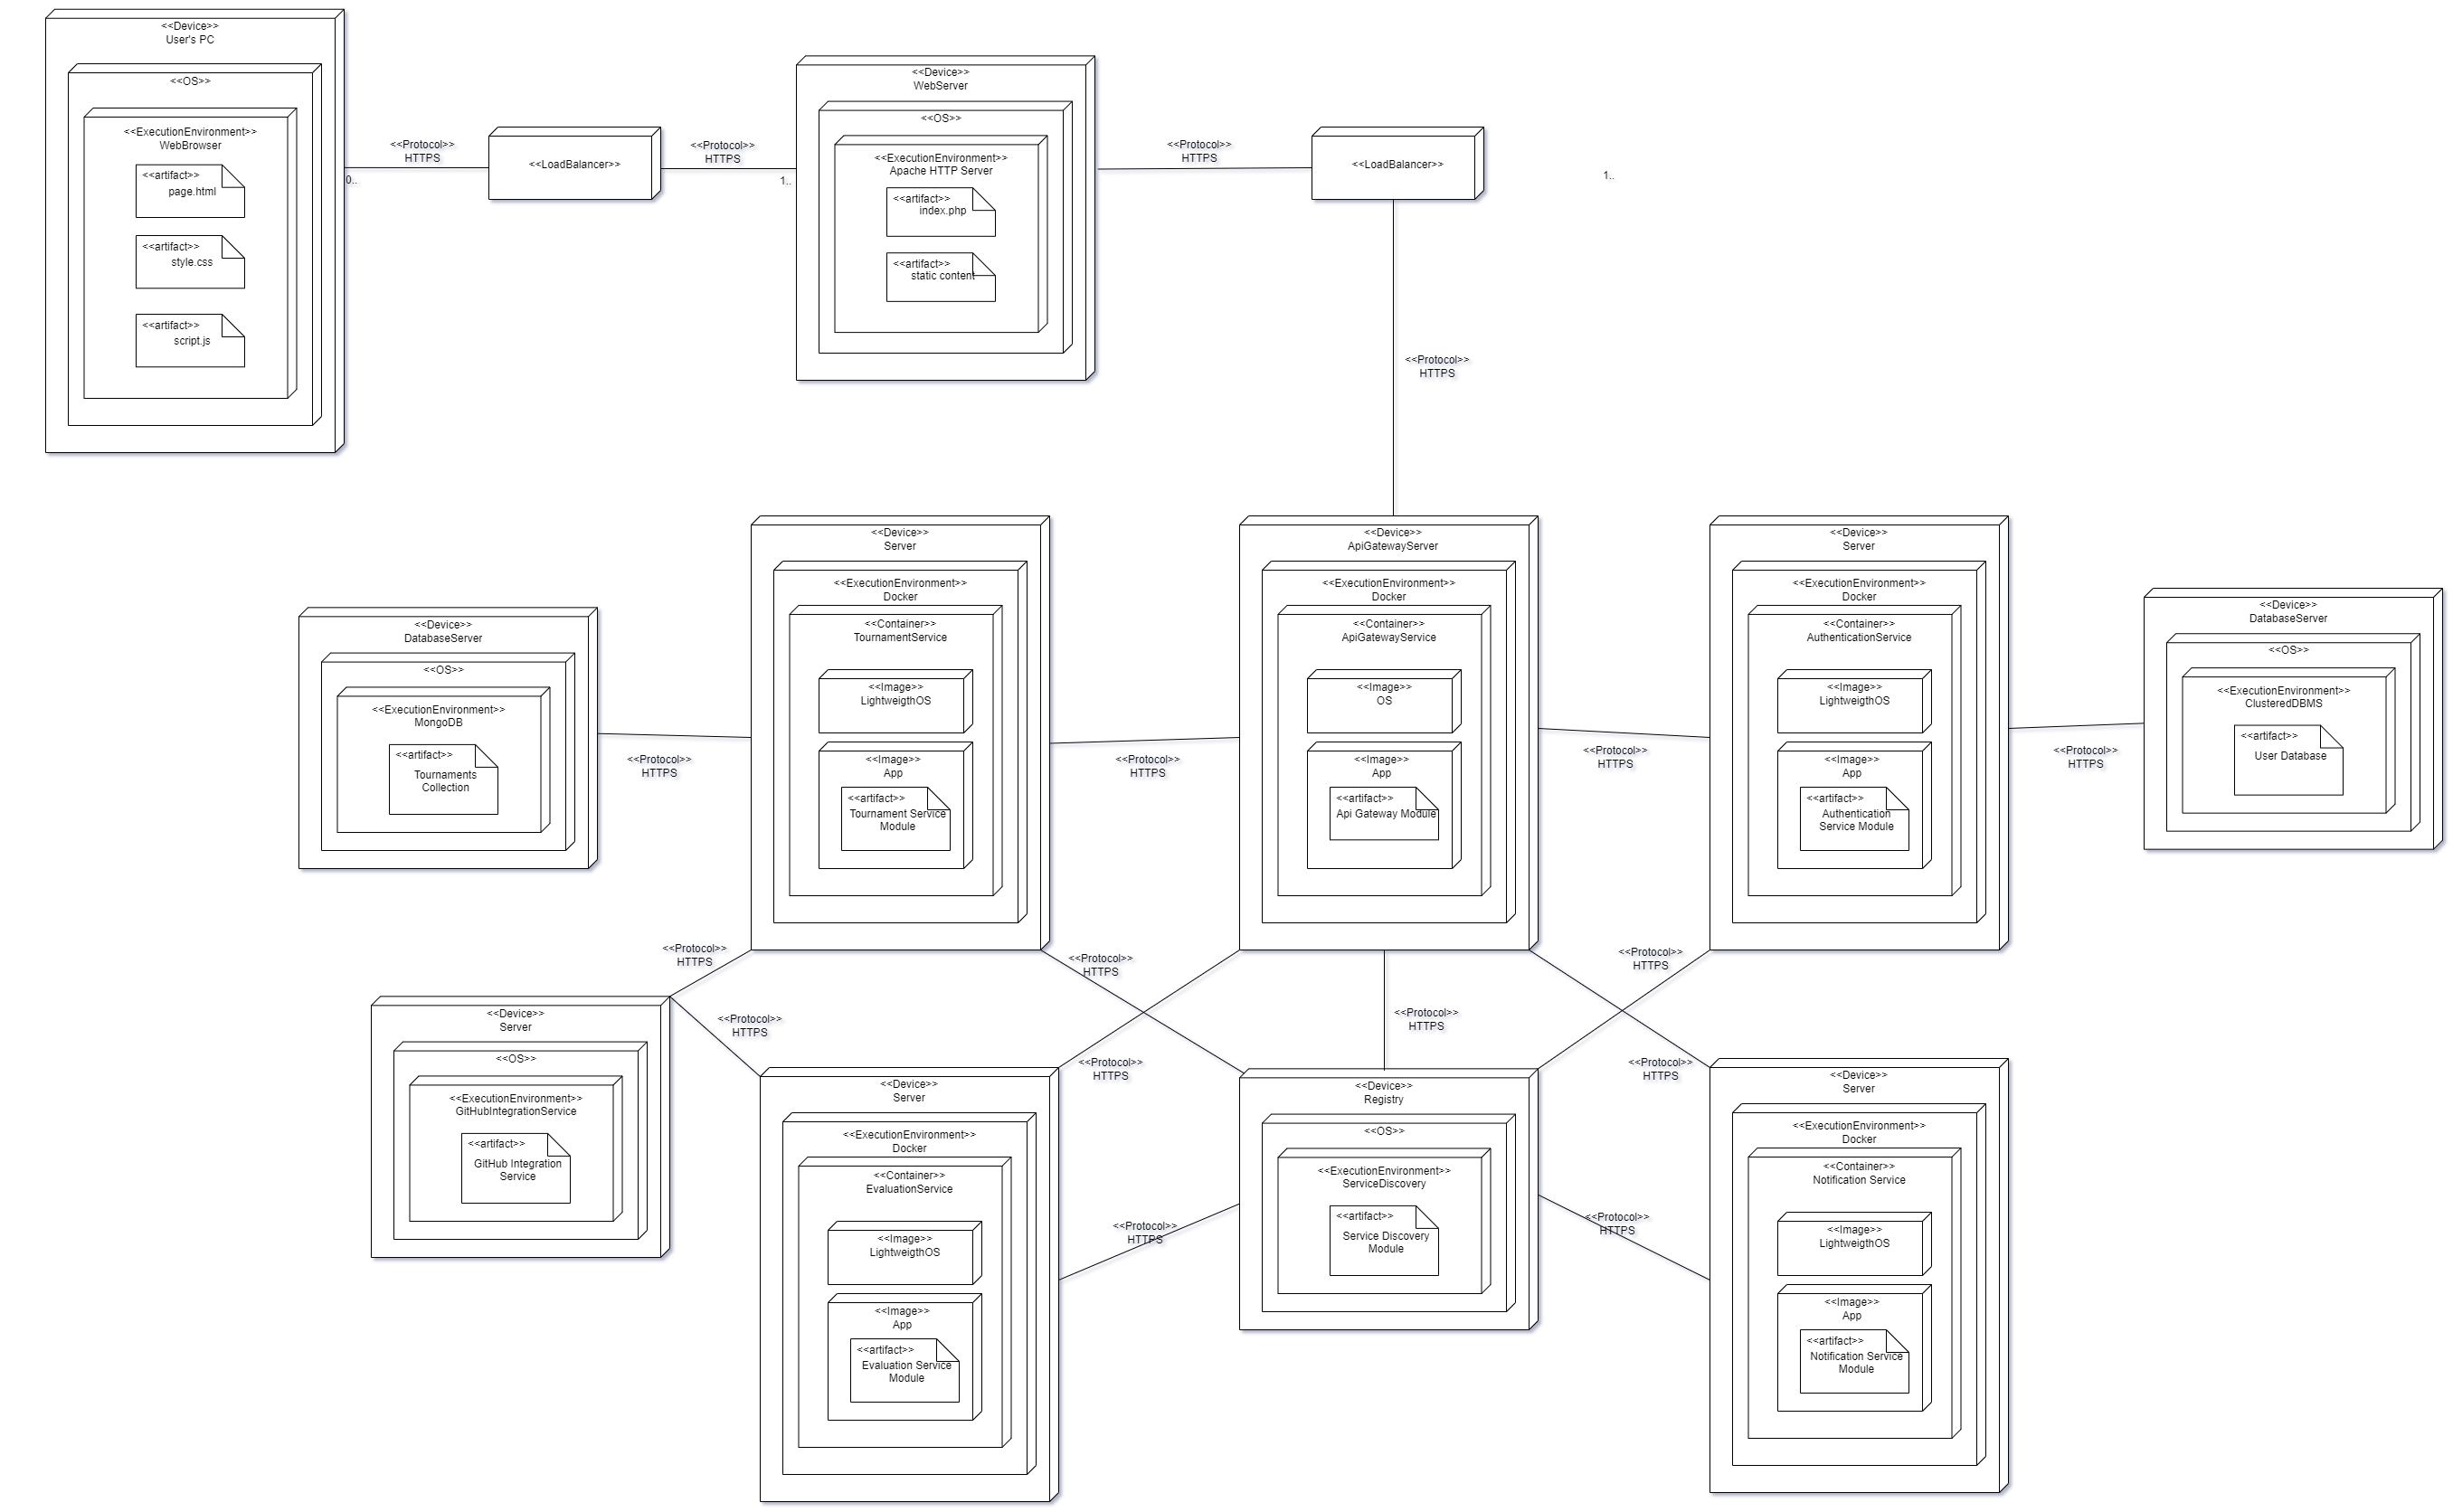
\includegraphics[width=1.1\textwidth]{Diagrams/deployment_diagram.png}
    \caption{Deployment diagram}
    \label{deployment_diagram}
\end{figure}

\subsection{Component interfaces}
The interfaces of the system's components are described in terms of the methods they offer, the parameters they require and the type of the values they return:
\begin{itemize}
    \item \textbf{APIGatewayI}
    \begin{itemize}
        \item login(credentials): userId
        \item loginSSO(identityProvider,ssoToken): userId
        \item signup(credentials,userType): userId
        \item signupSSO(identityProvider,ssoToken,userType): userId
        \item createBattle(userId,tournamentId,battleData): bool
        \item getTournaments(): tournamentDataList
        \item getEnrolledTournaments(userId): tournamentsDataList
        \item createTeam(userId,battleId,teamName,teamPrivacy): bool
        \item joinTeam(userId,battleId,joinOption,joinTextInput): bool
        \item readTeamSettings(userId,tournamentId,battleId,teamId): teamData
        \item updateTeamSettings(userId,tournamentId,battleId,teamId,gitHubRepoUrl): bool
        \item getTournamentRank(tournamentId): tournamentRank
        \item getBattleRank(battleId): battleRank
        \item getTeamSubmissions(userId,tournamentId,battleId,teamId): submissionsDataList
        \item joinTournament(userId,tournamentId): bool
        \item createTournament(userId,tournamentData): bool
        \item setManualScore(userId,teamId,score): bool
        \item closeBattleConsolidationPhase(userId,tournamentId,battleId): bool
        \item addCollaborator(userId,tournamentId,collaboratorEmail): bool
        \item closeTournament(userId,tournamentId): bool
    \end{itemize}
    \newpage
    \item \textbf{Auth2GatewayI}
    \begin{itemize}
        \item authenticateUser(credentials): userId
        \item createUser(credentials,userType): userId
        \item completeLoginSSO(identityProvider,ssoToken): userId
        \item completeSignupSSO(identityProvider,ssoToken,userType): userId
        \item getUserType(userId): userType
        \item getUserDataByEmail(userEmail): userData
    \end{itemize}
    \item \textbf{UserModelI}
    \begin{itemize}
        \item retrieveUserId(credentials): userId
        \item createUser(credentials, userType): userId
        \item retrieveUserData(userId): userData
        \item retrieveUsersData(userIdList): userDataList
        \item retrieveUserType(userId): userType
        \item retrieveUserDataByEmail(userEmail): userData
        \item retrieveAllStudentsData(): usersDataList
    \end{itemize}
    \item \textbf{Auth2EventI}
    \begin{itemize}
        \item getUserData(userId): userData
        \item getUsersData(userIdList): userDataList
        \item getAllStudentsData(): usersDataList
    \end{itemize}
    \item \textbf{CommitI}
    \begin{itemize}
        \item notifySubmission(teamId): none
    \end{itemize}
    \item \textbf{Tournament2GatewayI}
    \begin{itemize}
        \item createBattle(userId,tournamentId,battleData): bool
        \item setManualScore(userId,teamId,score): bool
        \item getTournaments(): tournamentDataList
        \item getTournamentRank(tournamentId): tournamentRank
        \item getBattleRank(battleId): battleRank
        \item getEnrolledTournaments(userId): tournamentsDataList
        \item createTeam(userId,battleId,teamName,teamPrivacy): bool
        \item joinTeam(userId,battleId,joinOption,joinTextInput): bool
        \item readTeamSettings(userId,tournamentId,battleId,teamId): teamData
        \item updateTeamSettings(userId,tournamentId,battleId,teamId,gitHubRepoUrl): bool
        \item getTeamSubmissions(userId,tournamentId,battleId,teamId): submissionsDataList
        \item joinTournament(userId,tournamentId): bool
        \item createTournament(userId,tournamentData): bool
        \item closeBattleConsolidationPhase(userId,tournamentId,battleId): bool
        \item addCollaborator(userId,tournamentId,collaboratorEmail,collaboratorId): bool
        \item closeTournament(userId,tournamentId): bool
    \end{itemize}
    \item \textbf{Tournament2EventI}
    \begin{itemize}
        \item getTournamentUsers(tournamentId): userIdList
        \item getKataData(battleId): codeKataData
        \item getBattleStudents(battleId): userIdList
        \item getTeamStudents(teamId): userIdList
        \item setNextBattleState(battleId): none
        \item closeTournamentSubscriptionPhase(tournamentId): none
        \item endBattle(battleId): none
        \item updateBattleRank(tournamentId,battleId,battleRank): none
        \item endTournament(tournamentId): none
    \end{itemize}
    \item \textbf{Tournament2EvaluationI}
    \begin{itemize}
        \item setAutomaticScore(teamId,scores): none
        \item getTeamRepoUrl(teamId): repoUrl
        \item getBattleByTeamId(teamId): battleId
        \item getBattleSettings(battleId): battleSettings
        \item notifyTeamEvaluation(teamId): none
        \item getBattleDataByTeamId(teamId): battleData
    \end{itemize}
    \item \textbf{TournamentModelI}
    \begin{itemize}
        \item retrieveEducators(tournamentId): userIdList
        \item retrieveKataData(battleId): codeKataData
        \item retrieveBattleCreator(battleId): userId
        \item retrieveTournamentCreator(tournamentId): userId
        \item retrieveBattleStudents(battleId): userIdList
        \item retrieveTeamRepoUrl(teamId): repoUrl
        \item retrieveTeamStudents(teamId): userIdList
        \item setAutomaticScore(teamId,scores): none
        \item setManualScore(teamId,score): bool
        \item retrieveTournaments(): tournamentsDataList
        \item retrieveTournamentByBattle(battleId): tournamentData
        \item retrieveTournamentUsers(tournamentId): userIdList
        \item retrieveTournamentState(tournamentId): tournamentState
        \item retrieveBattleState(battleId): battleState
        \item retrieveEnrolledTournaments(userId): tournamentsDataList
        \item setBattleState(battleId,state): none
        \item createBattle(userId,tournamentId,battleData): battleId
        \item retrieveBattleByTeamId(teamId): battleId
        \item retrieveBattleSettings(battleId): battleSettings
        \item createTeam(userId,tournamentId,battleId,teamName,teamPrivacy): bool
        \item addStudentToTeam(userId,tournamentId,battleId,teamId): none
        \item retrieveTeamData(tournamentId,battleId,teamId): teamData
        \item updateTeamData(tournamentId,battleId,teamId,gitHubRepoUrl): bool
        \item retrieveTournamentRank(tournamentId): tournamentRank
        \item retrieveBattleRank(battleId): battleRank
        \item updateBattleRank(battleId,battleRank): none
        \item retrieveTeamSubmissions(tournamentId,battleId,teamId): submissionsDataList
        \item addStudentToTournament(userId,tournamentId): none
        \item createTournament(userId,tournamentData): tournamentId
        \item setTournamentState(tournamentId,tournamentState): none
        \item retrieveBattleData(tournamentId,battleId): battleData
        \item retrieveTournamentData(tournamentId): tournamentData
        \item updateTournamentRankAndScores(tournamentId,tournamentRank,tournamentScores): none
        \item updateBattleRank(tournamentId,battleId,battleRank): none
        \item addCollaborator(tournamentId,collaboratorId): none
        \item retrieveBattleDataByTeamId(teamId): battleData
    \end{itemize}
    \item \textbf{PushEventI}
    \begin{itemize}
        \item push(event): bool
    \end{itemize}
    \item \textbf{PullEventI}
    \begin{itemize}
        \item fetchHeadTimestamp(): timestamp
        \item pull(): event
    \end{itemize}
    \item \textbf{CreateRepositoryI}
    \begin{itemize}
        \item createRepo(repoData): none
    \end{itemize}
    \item \textbf{RetrieveSubmissionCodeI}
    \begin{itemize}
        \item retrieveRepo(repoUrl): code
    \end{itemize}
    \newpage
    \item \textbf{PushSubmissionI}
    \begin{itemize}
        \item push(teamId): bool
    \end{itemize}
    \item \textbf{PullSubmissionI}
    \begin{itemize}
        \item isEmpty(): bool
        \item pull(): teamId
    \end{itemize}
    \item \textbf{PushNotificationI}
    \begin{itemize}
        \item push(notification): bool
    \end{itemize}
    \item \textbf{PullNotificationI}
    \begin{itemize}
        \item isEmpty(): bool
        \item pull(): notification
    \end{itemize}
    \item \textbf{RegistryI}
    \begin{itemize}
        \item getInstance(serviceType): instanceUrl
        \item subscribeInstance(serviceType,instanceUrl): bool
        \item heartbeat(serviceType,instanceUrl): bool
    \end{itemize}
\end{itemize}

The system's components will exploit the following APIs, provided by already existing services or components:
\begin{itemize}
    \item \textbf{TournamentDBMS API}
    \item \textbf{UserDBMS API}
    \item \textbf{SSO API}:
    \begin{itemize}
        \item checkToken(ssoToken): userData
        \item initializeSSO(ssoCredentials): ssoToken
    \end{itemize}
    \item \textbf{GitHub API}: 
    \begin{itemize}
        \item createRepo(repoData): none
        \item retrieveRepo(repoUrl): code
    \end{itemize}
    \item \textbf{StaticAnalysis API}: 
    \begin{itemize}
        \item analyze(code,qualityAspect): score
    \end{itemize}
    \item \textbf{Email API}:
    \begin{itemize}
        \item sendEmail(recipientEmail,object,body): none
    \end{itemize}
\end{itemize}
This representation of the system's interfaces is only for illustrative purposes: actual function calls will be performed through proper HTTP requests in which parameters will be included in the request body and the response will be encoded in JSON format. This is allowed by the use of REST APIs, as described in the next section.

\newpage
\subsection{Runtime view}
TODO: check for missing text\\
In this section the most important runtime scenarios of the system are presented, highlighting the interactions between different components and, eventually, external entities.

For the sake of brevity, the retrival of dynamic content used to populate the pages rendered by the web server is not shown, so that only the most important exchanges can be represented.

\subsubsection{Service Registry}
The Service Registry is a critical component of the system, since it is responsible for the service discovery functionality, on which the microservice architecture is based. This is achieved by allowing 3 fundamental operations:
\begin{itemize}
    \item \textbf{Service registration}: each microservice instance can register itself to the Service Registry, specifying the type of service it provides and its URL.
    \begin{figure}[H]
        \centering
        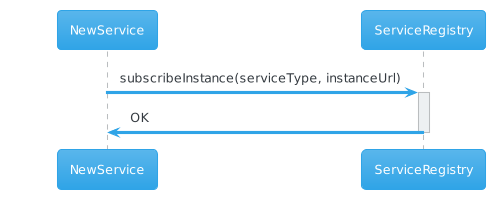
\includegraphics[width=0.8\textwidth]{Diagrams/sequence/service_registration.png}
        \caption{Service registration}
    \end{figure}
    \item \textbf{Service discovery}: each microservice instance can query the Service Registry to retrieve the URL of an instance of a specific type.
    \begin{figure}[H]
        \hspace{2cm}
        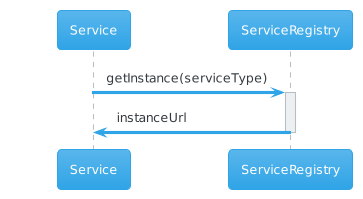
\includegraphics[width=0.6\textwidth]{Diagrams/sequence/service_discovery.png}
        \caption{Service discovery}
    \end{figure}
    \item \textbf{Heartbeat}: each microservice instance periodically sends a heartbeat to the Registry to notify that it is still alive and update its availability status.
    \begin{figure}[H]
        \centering
        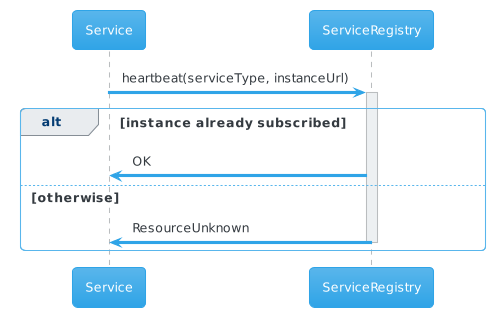
\includegraphics[width=0.8\textwidth]{Diagrams/sequence/service_heartbeat.png}
        \caption{Heartbeat reception}
    \end{figure}
\end{itemize}

\subsubsection{Signup}
\begin{figure}[H]
    \centering
    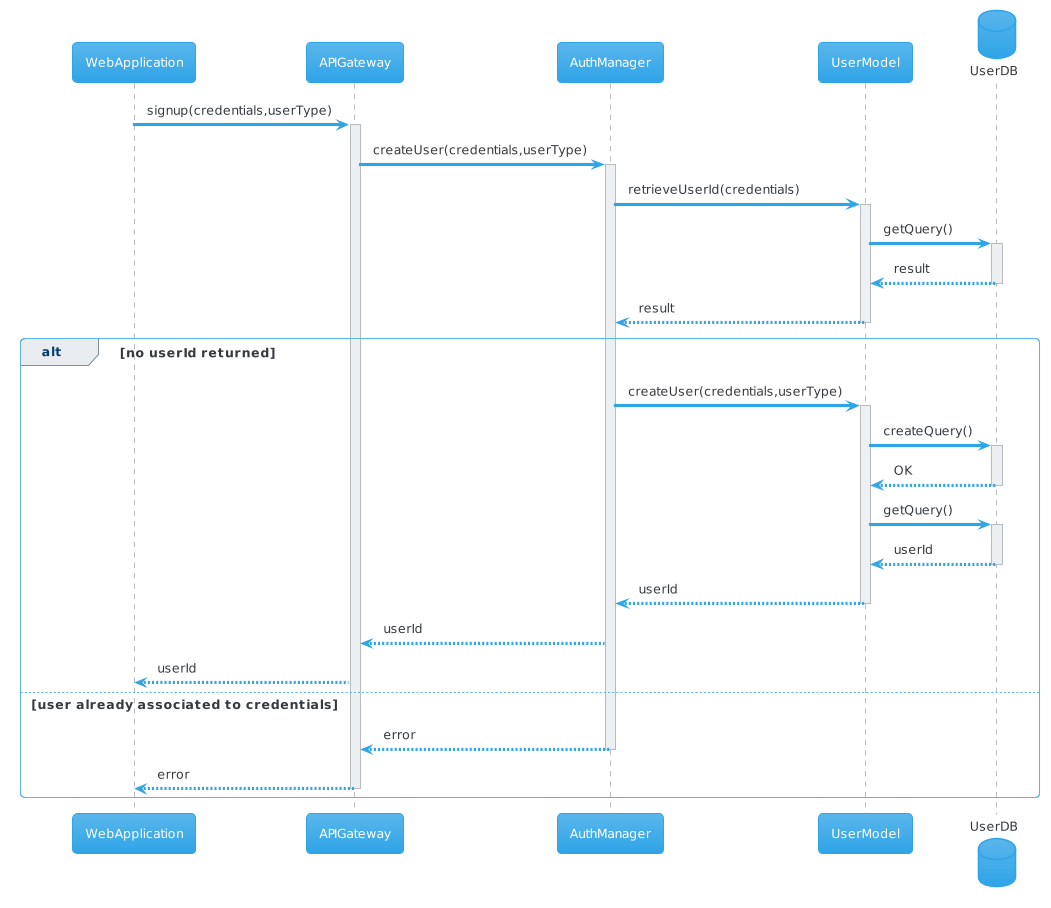
\includegraphics[width=1\textwidth]{Diagrams/sequence/signup.png}
    \caption{Normal sign up process}
\end{figure}
\begin{figure}[H]
    \hspace{-0.7cm}
    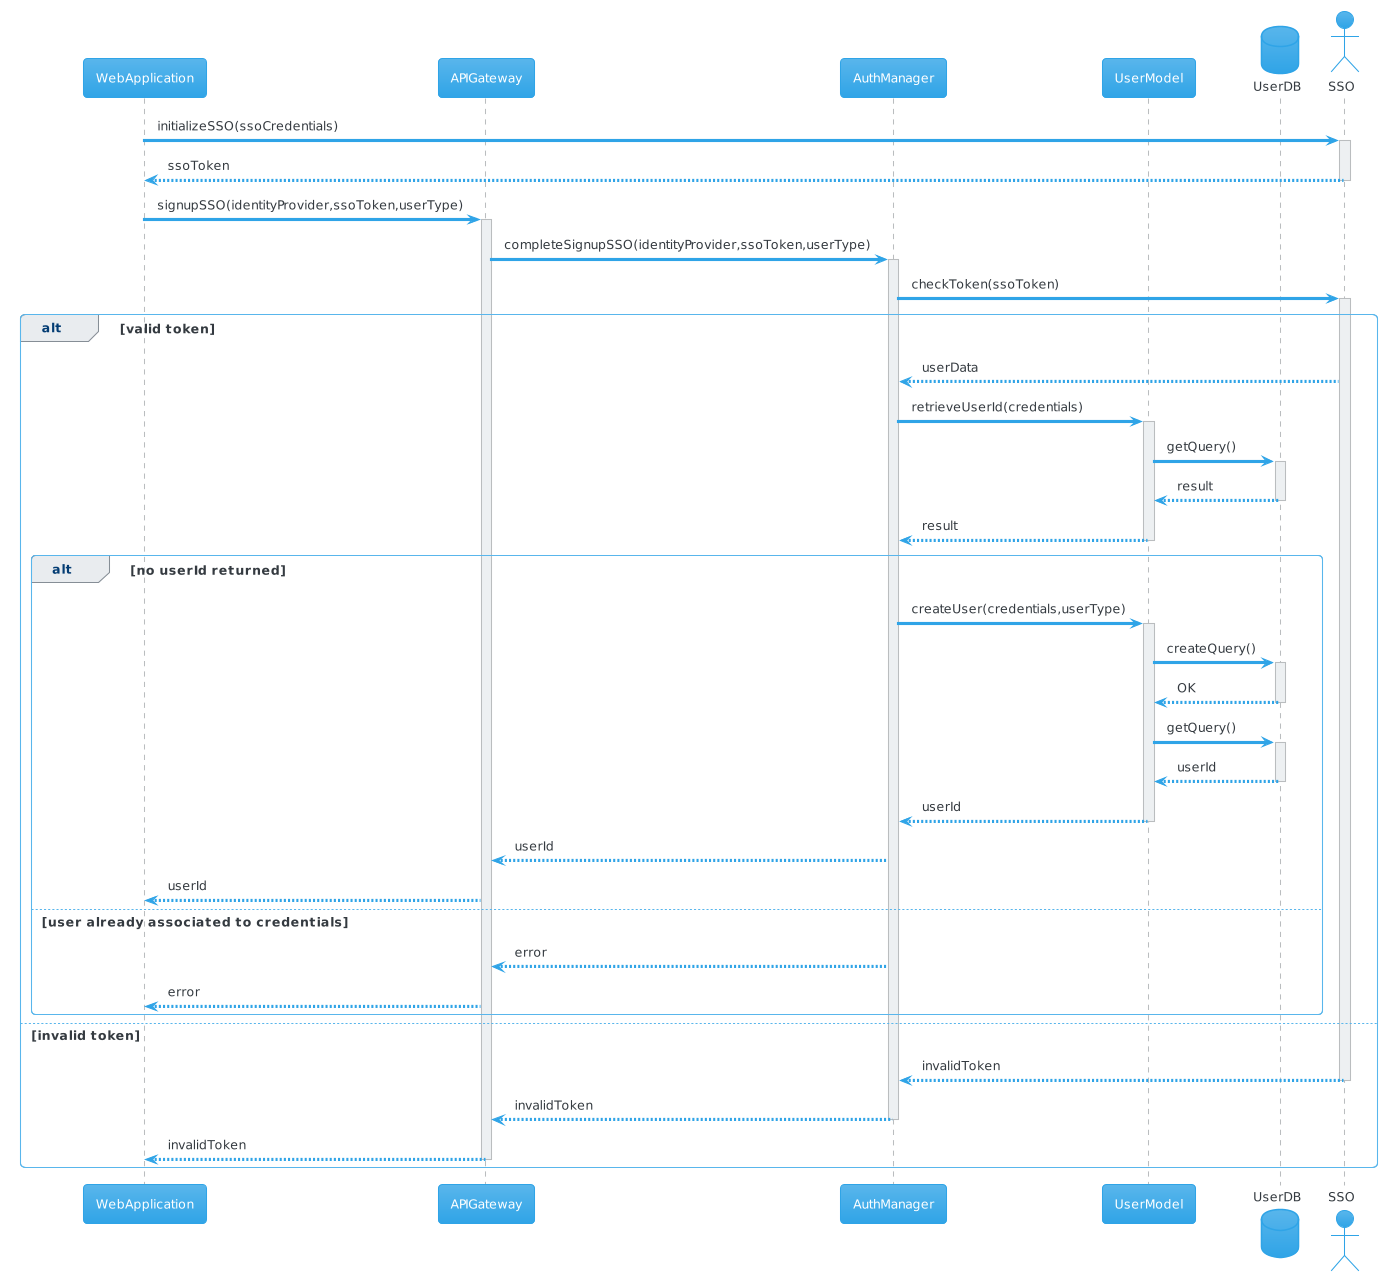
\includegraphics[width=1.1\textwidth]{Diagrams/sequence/signup_SSO.png}
    \caption{Sign up through SSO}
\end{figure}

\subsubsection{Login}
\begin{figure}[H]
    \centering
    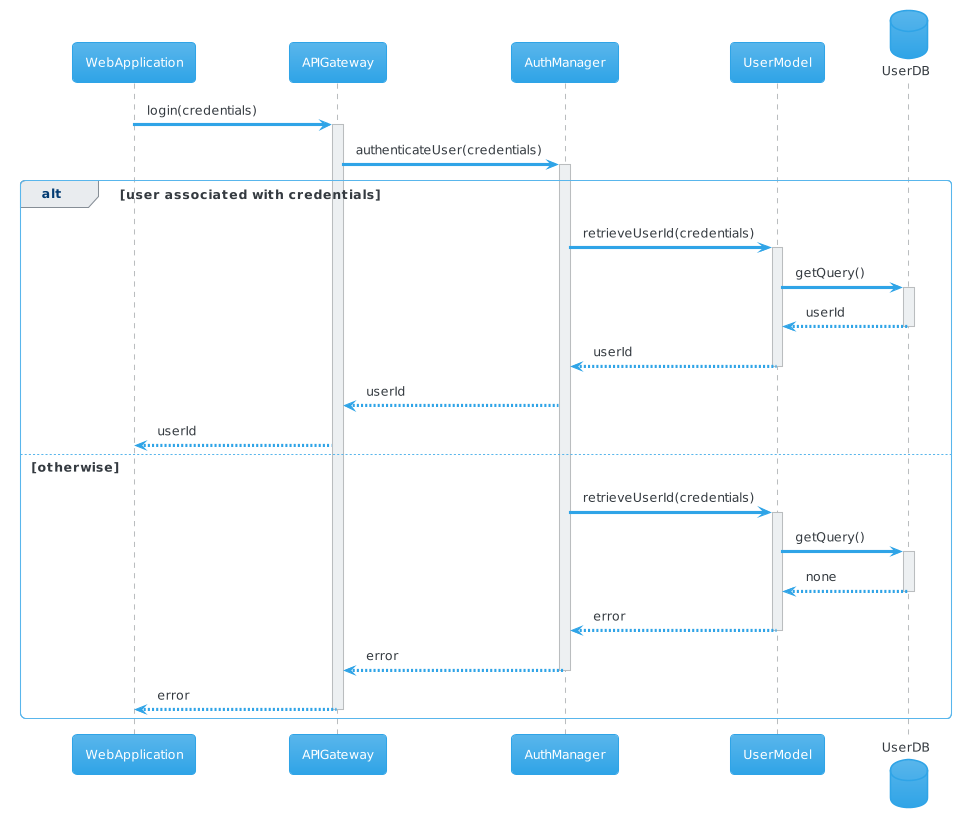
\includegraphics[width=1\textwidth]{Diagrams/sequence/login.png}
    \caption{Log in process}
\end{figure}
\begin{figure}[H]
    \hspace{-0.7cm}
    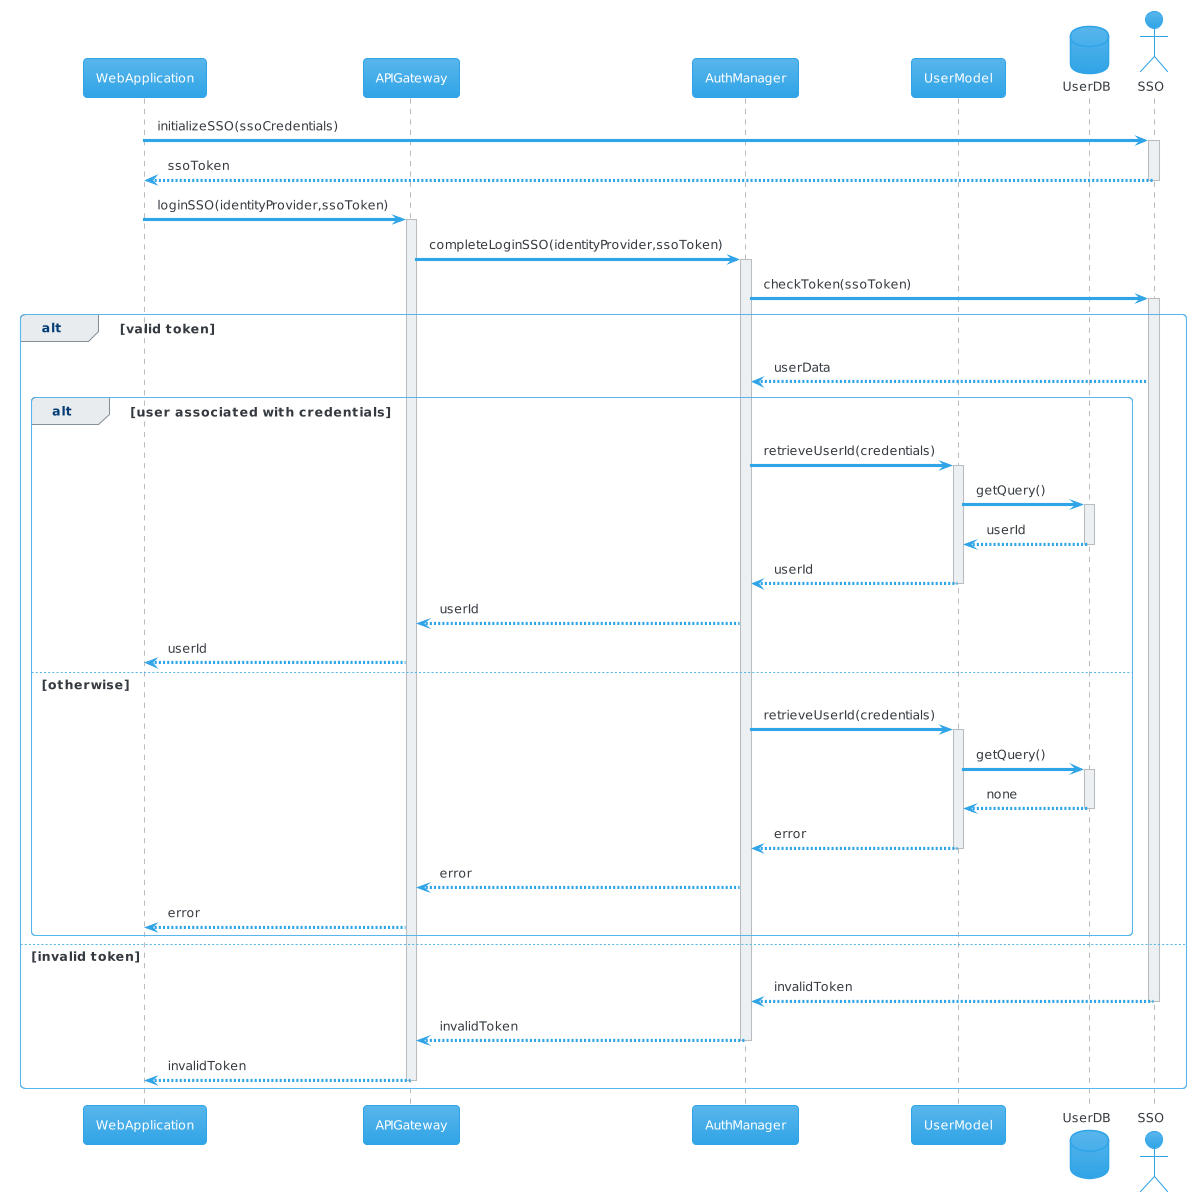
\includegraphics[width=1.1\textwidth]{Diagrams/sequence/login_SSO.png}
    \caption{Log in through SSO}
\end{figure}

\subsubsection{Create a tournament}
\begin{figure}[H]
    \hspace{-0.7cm}
    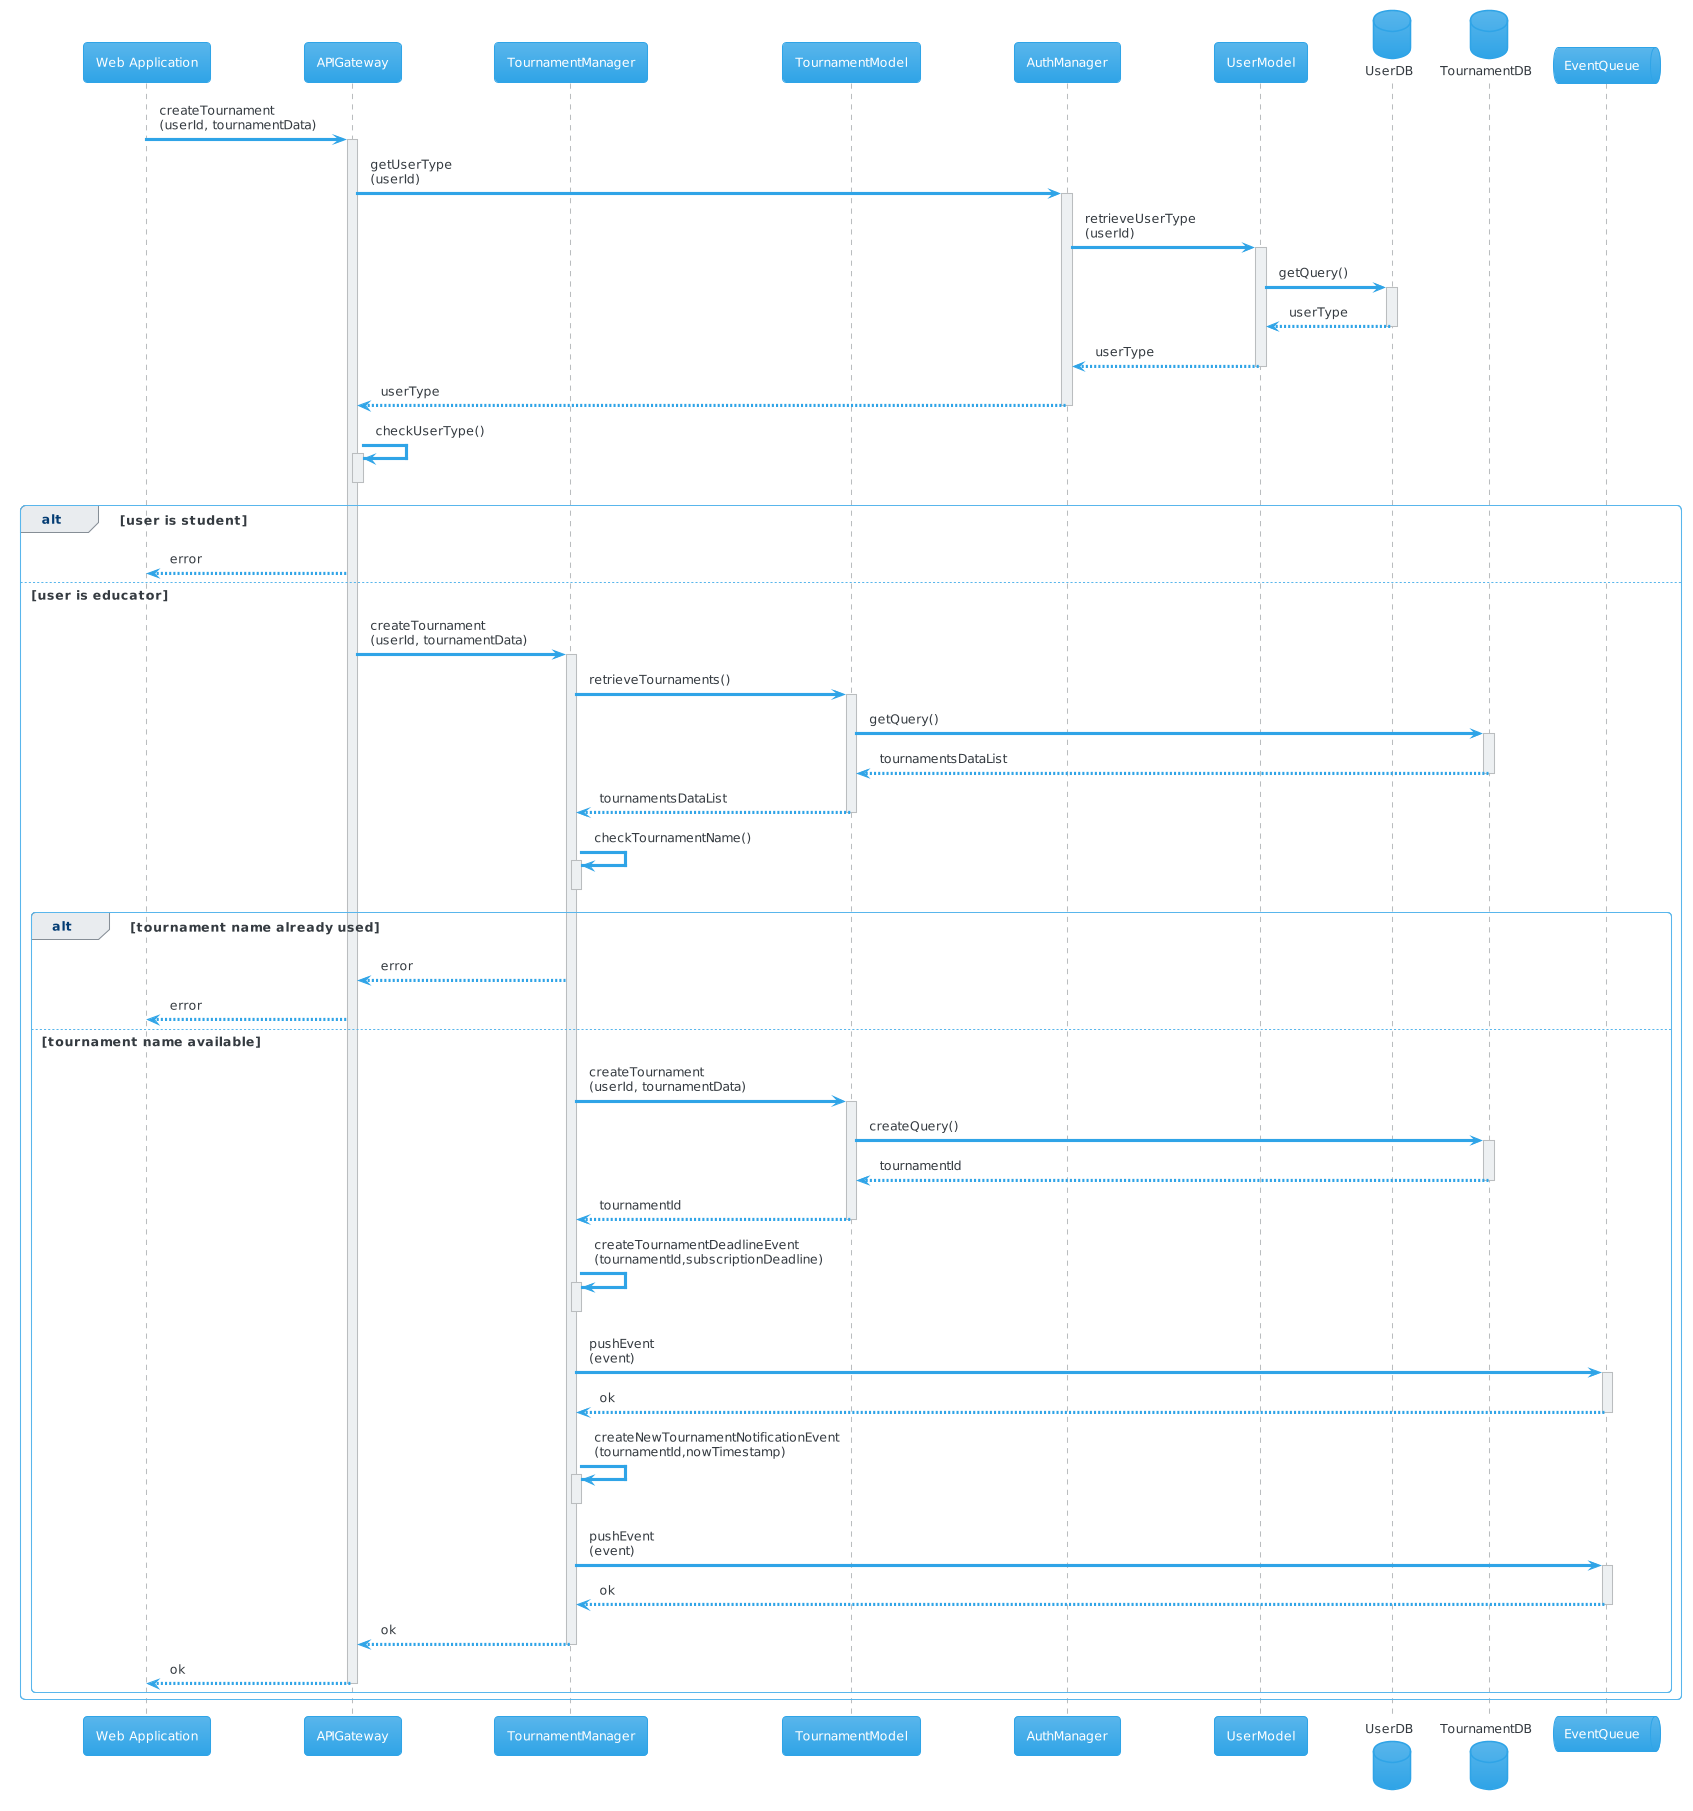
\includegraphics[width=1.1\textwidth]{Diagrams/sequence/create_tournament.png}
    \caption{Tournament creation process}
\end{figure}
As it will happen for many other use cases, the asynchronous communication framework used between specific services of the system has the effect of decoupling the components, allowing them to work independently in separated points in time. For this reason some of the scenarios have been completed with an additional sequence diagram in which is shown the Event Service pulling the event messages generated by the scenario, with all its effects.

Moreover, some system's processes will generate multiple messages, so the additional diagrams will be multiple as well, as in this case.
\begin{figure}[H]
    \hspace{-0.7cm}
    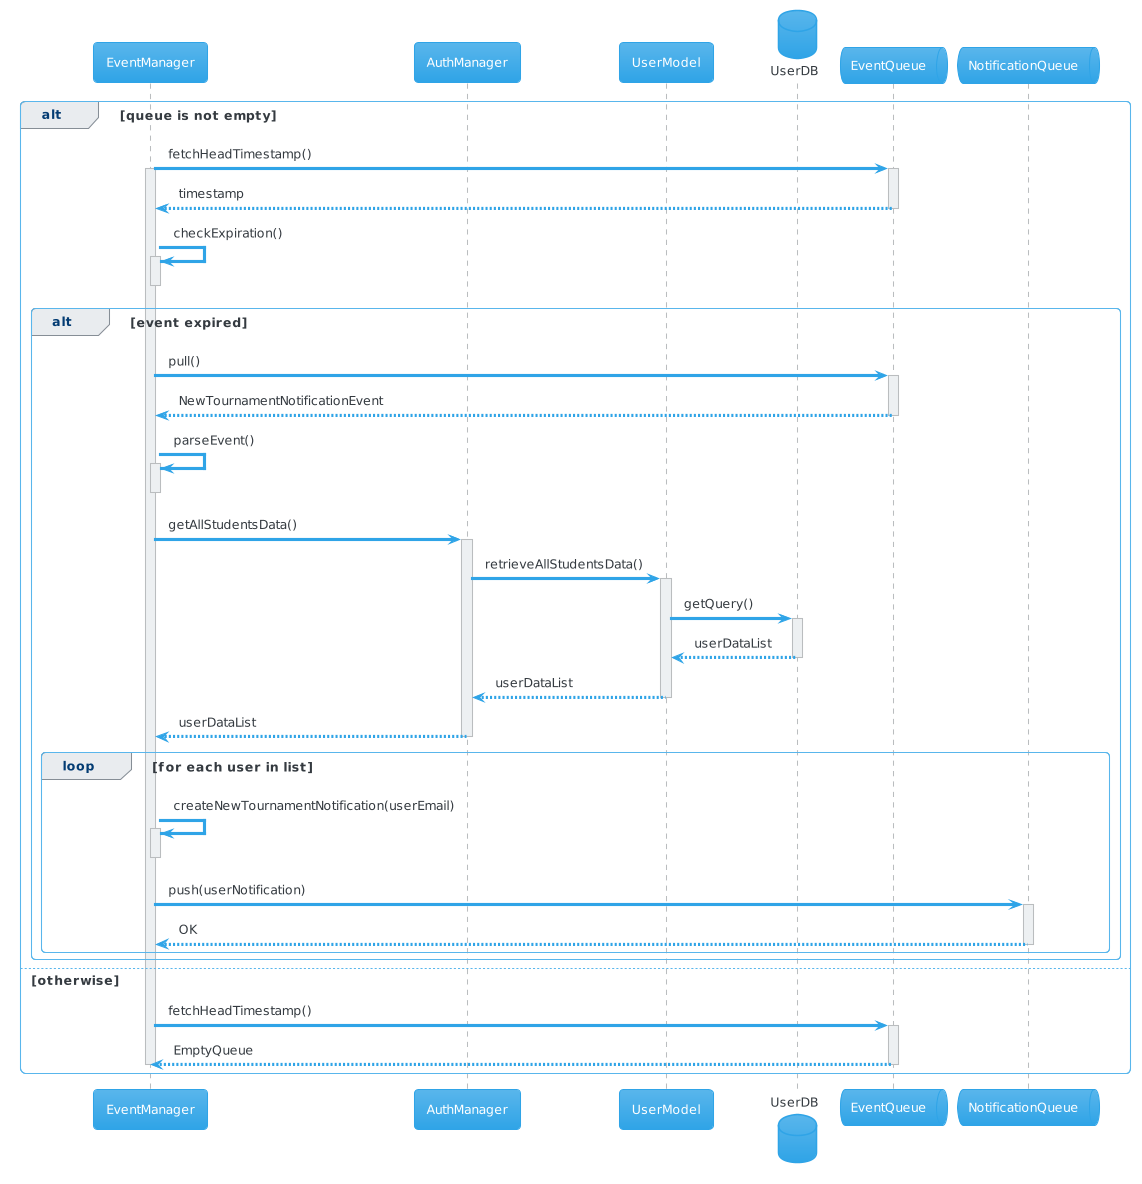
\includegraphics[width=1.1\textwidth]{Diagrams/sequence/create_tournament_pull_notification.png}
    \caption{Pull of the notification event generated by the tournament creation}
\end{figure}
\begin{figure}[H]
    \hspace{-0.7cm}
    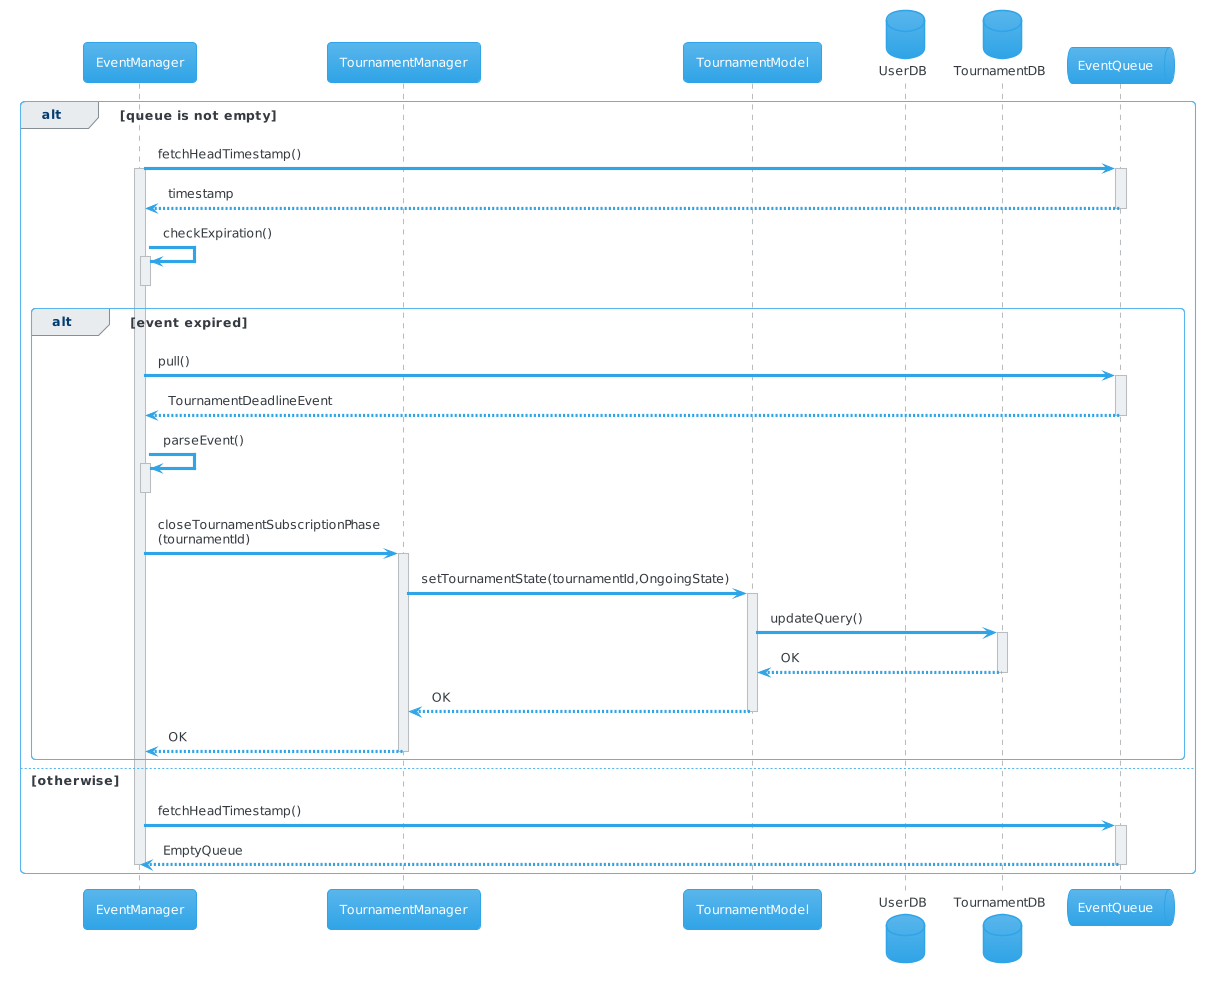
\includegraphics[width=1.1\textwidth]{Diagrams/sequence/create_tournament_pull_deadline.png}
    \caption{Pull of the deadline event, representing the end of the registration phase, generated by the tournament creation}
\end{figure}

\subsubsection{Add a collaborator to a tournament}
\begin{figure}[H]
    \hspace{-1.5cm}
    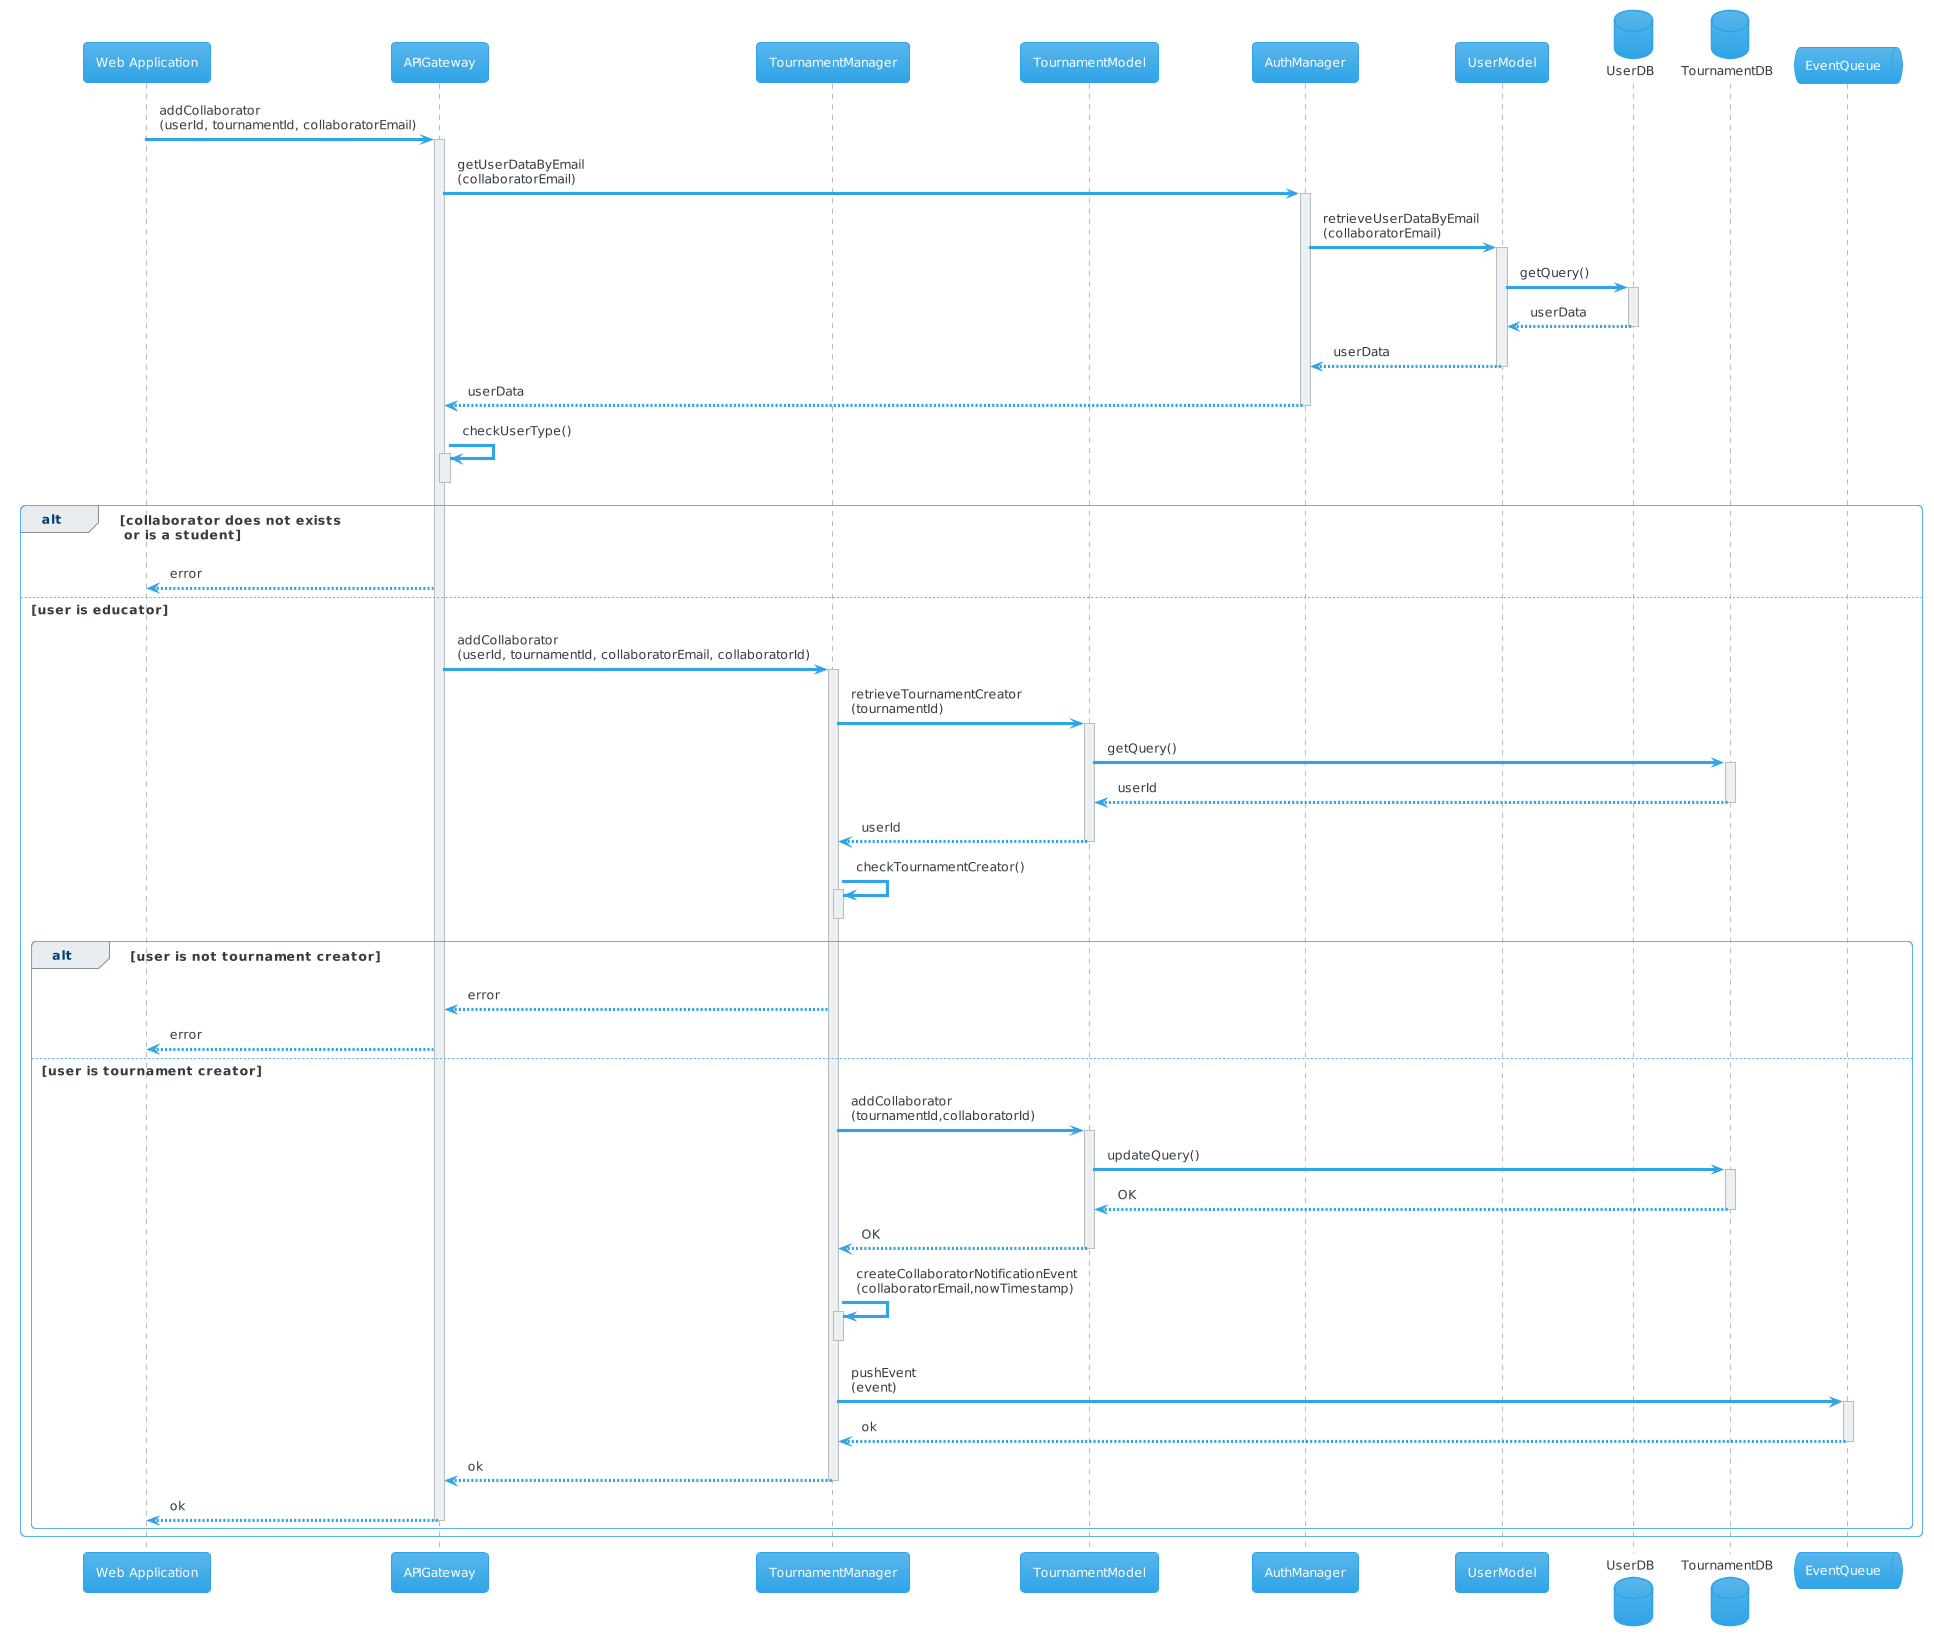
\includegraphics[width=1.2\textwidth]{Diagrams/sequence/add_collaborator.png}
    \caption{Process of adding a collaborator to a tournament}
\end{figure}
In this case the pull of the relative notification has not been represented since it would be very similar to what happens in the case of tournament creation.

\newpage
\subsubsection{Join a tournament}
\begin{figure}[H]
    \hspace{-1.5cm}
    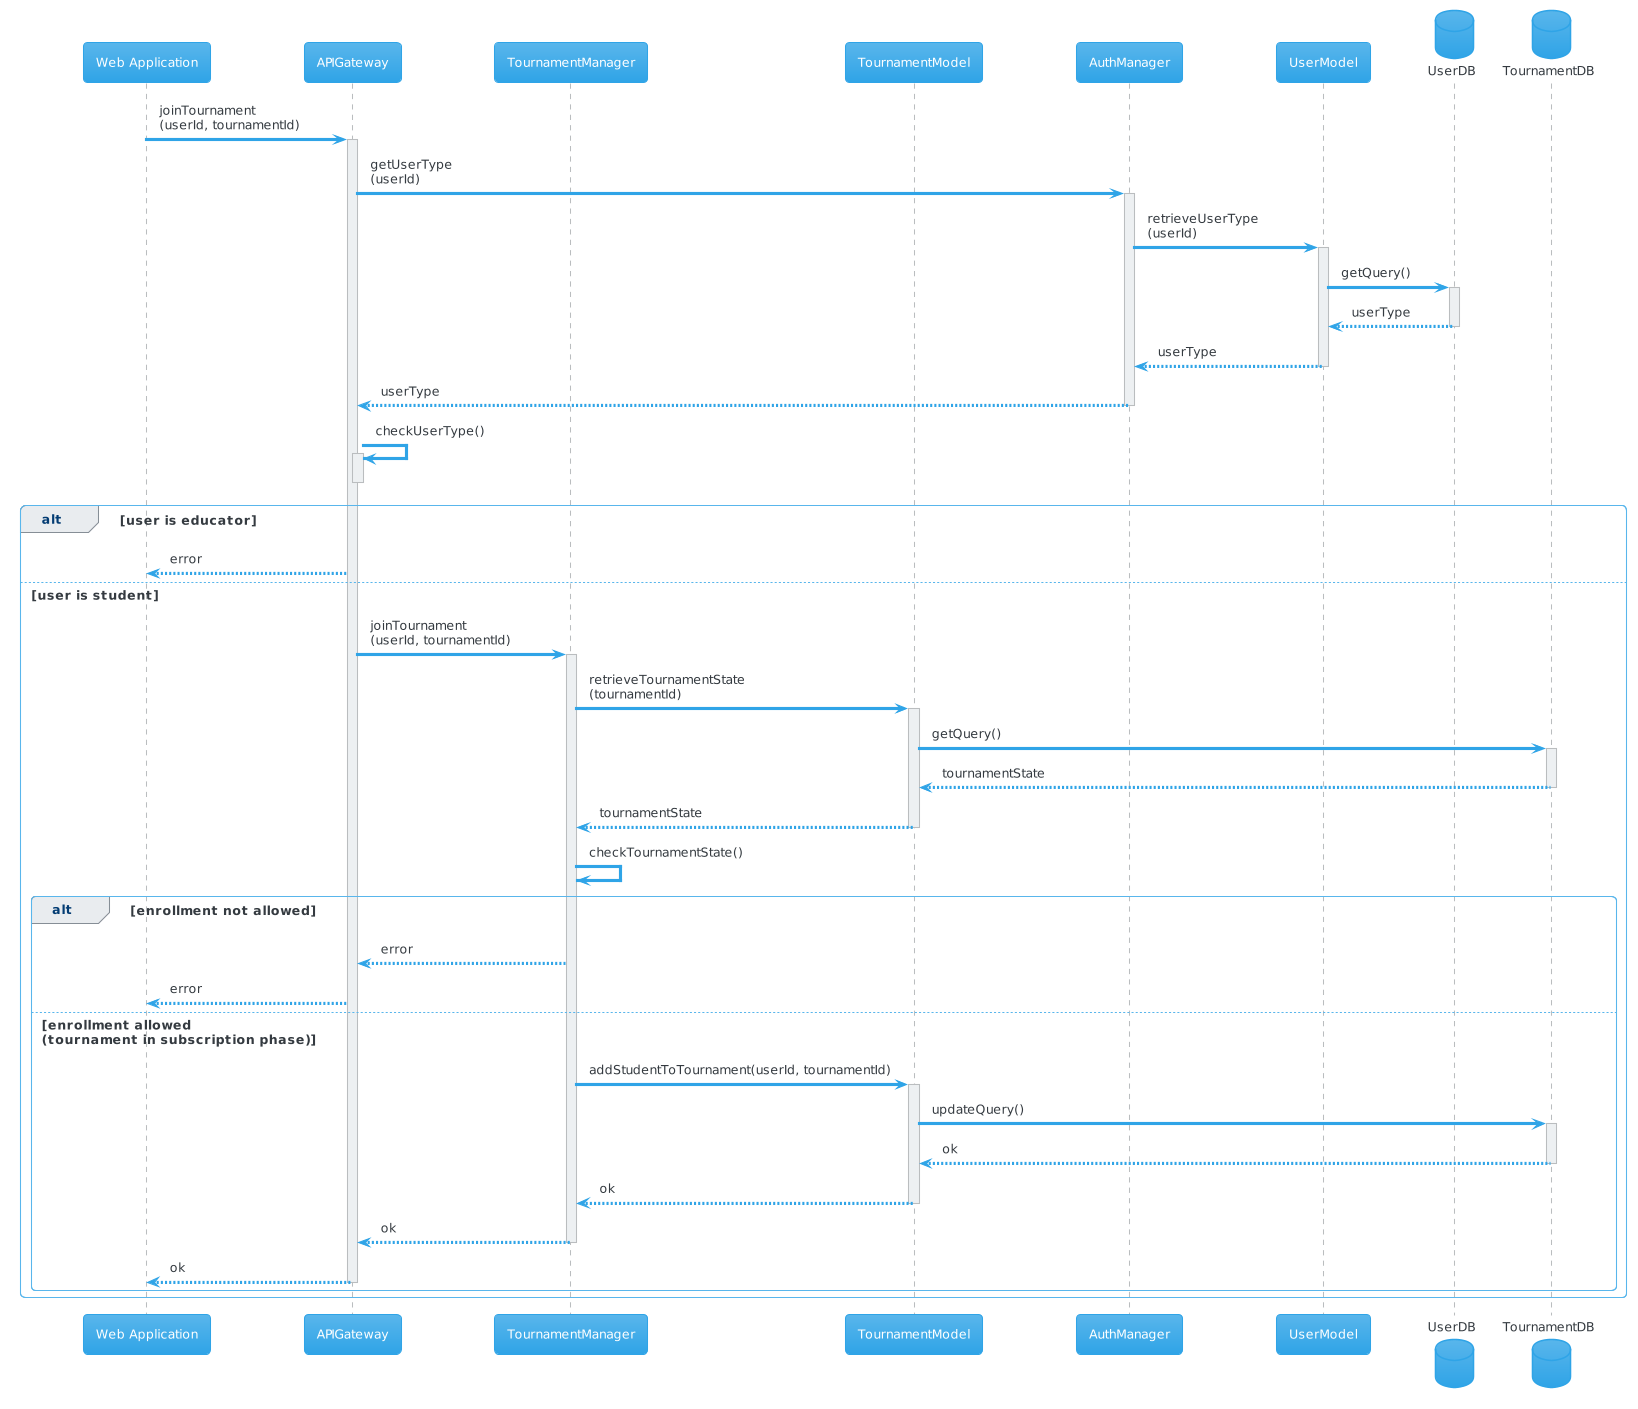
\includegraphics[width=1.2\textwidth]{Diagrams/sequence/join_tournament.png}
    \caption{Process of subscribing to a tournament}
\end{figure}

\subsubsection{Create a battle}
\begin{figure}[H]
    \hspace{-0.7cm}
    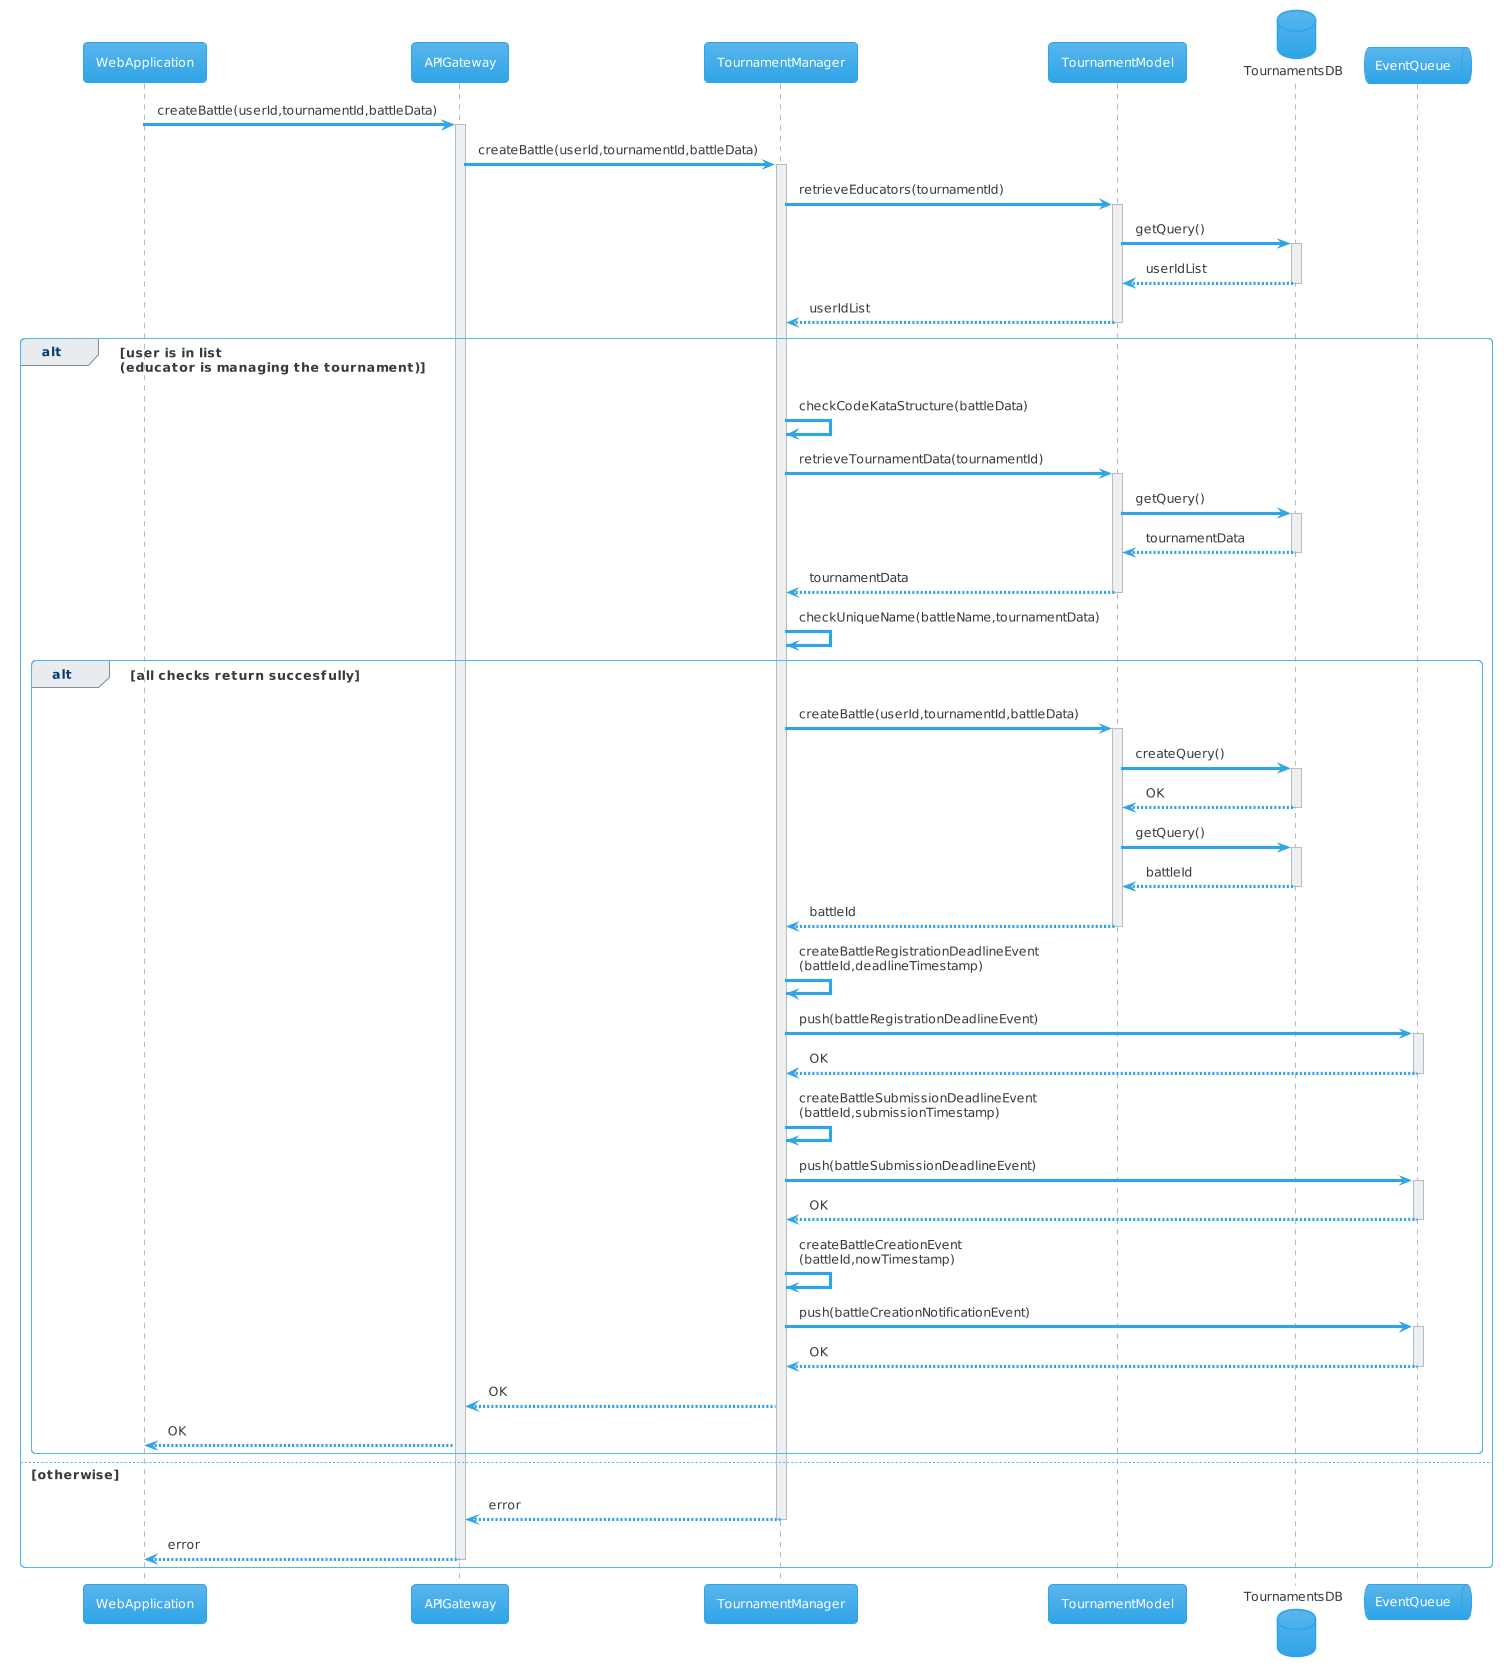
\includegraphics[width=1.1\textwidth]{Diagrams/sequence/create_battle.png}
    \caption{Battle creation process}
\end{figure}
\begin{figure}[H]
    \hspace{-1.5cm}
    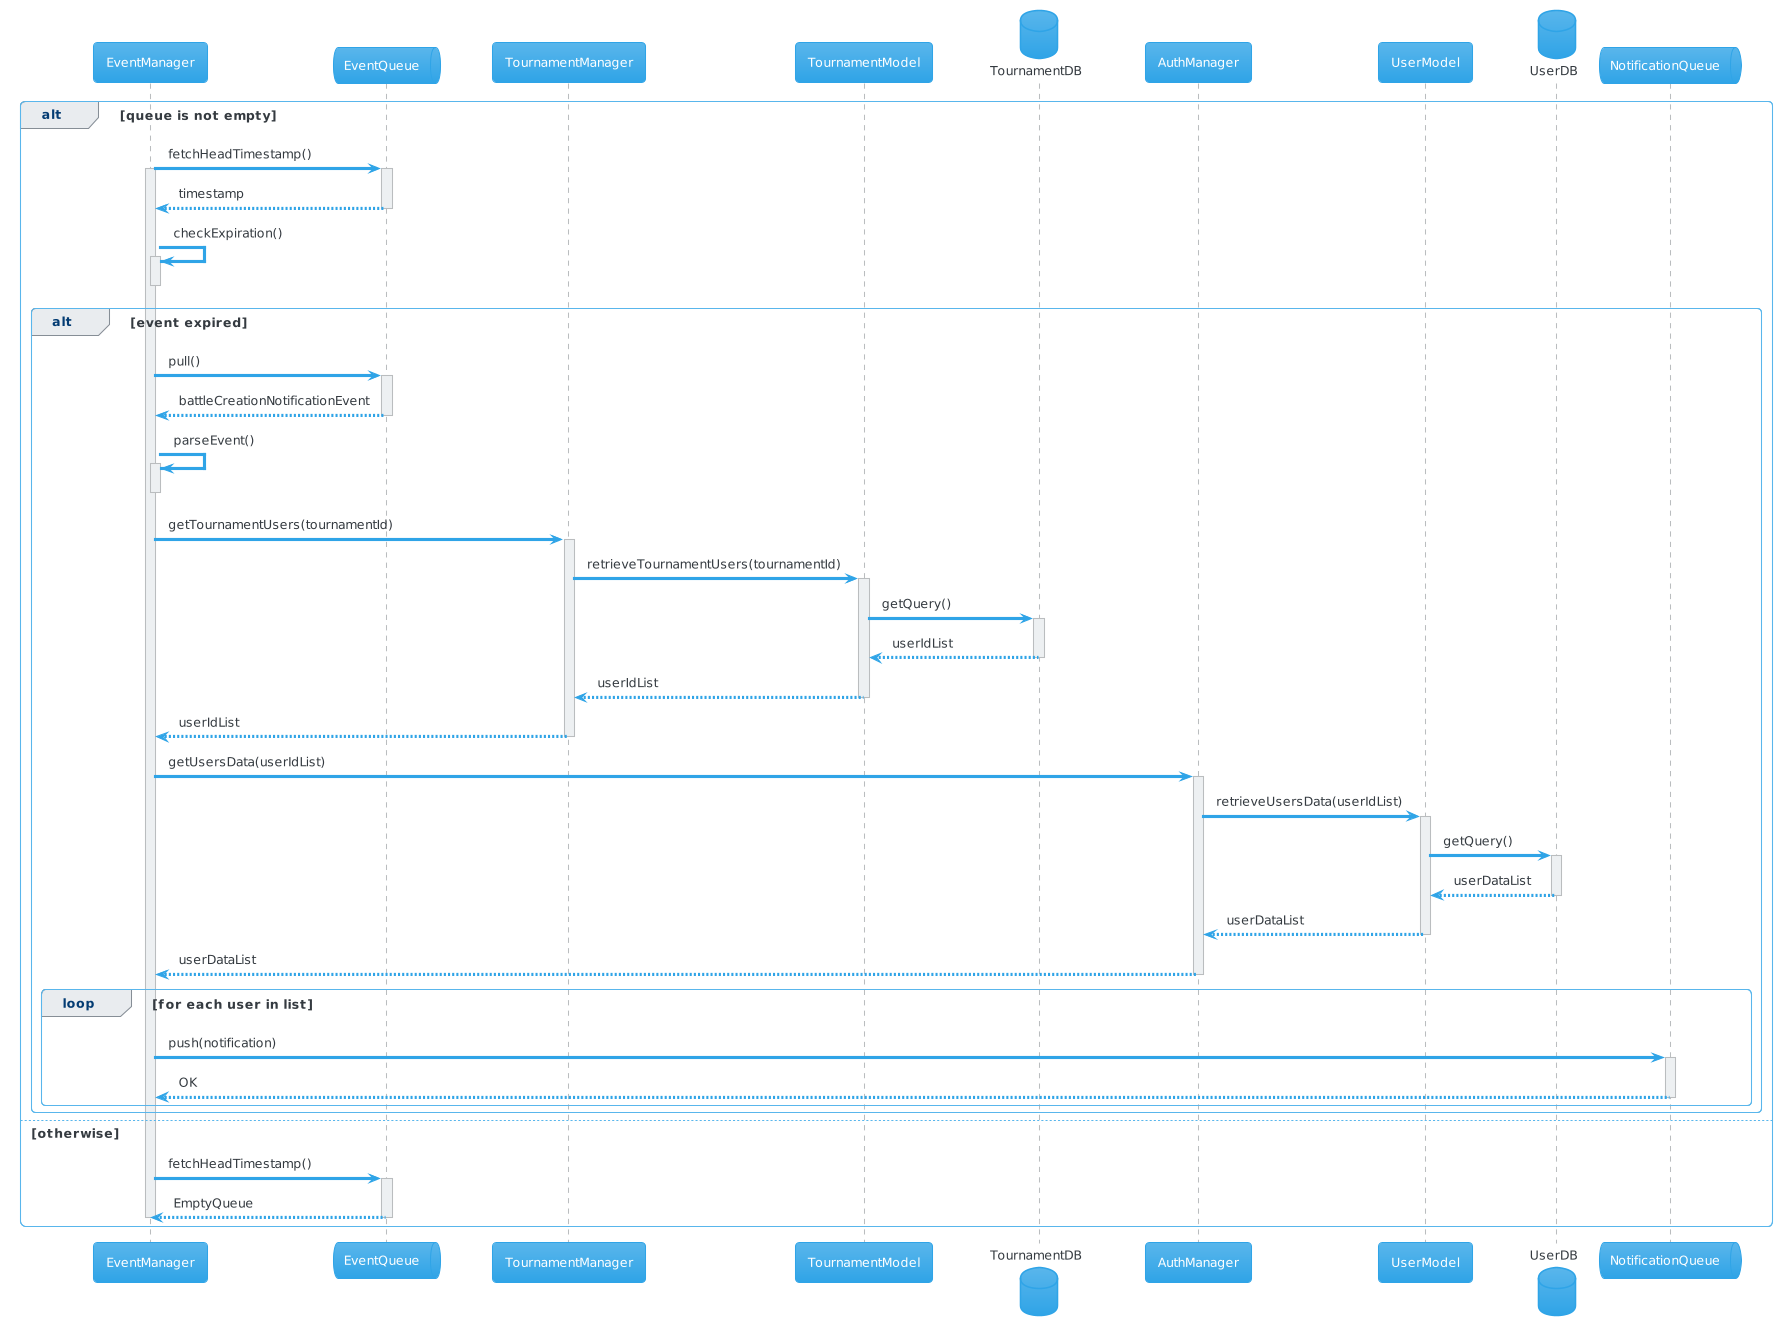
\includegraphics[width=1.2\textwidth]{Diagrams/sequence/create_battle_pull_notification.png}
    \caption{Pull of the notification event generated by the battle creation}
\end{figure}
\begin{figure}[H]
    \hspace{-1.5cm}
    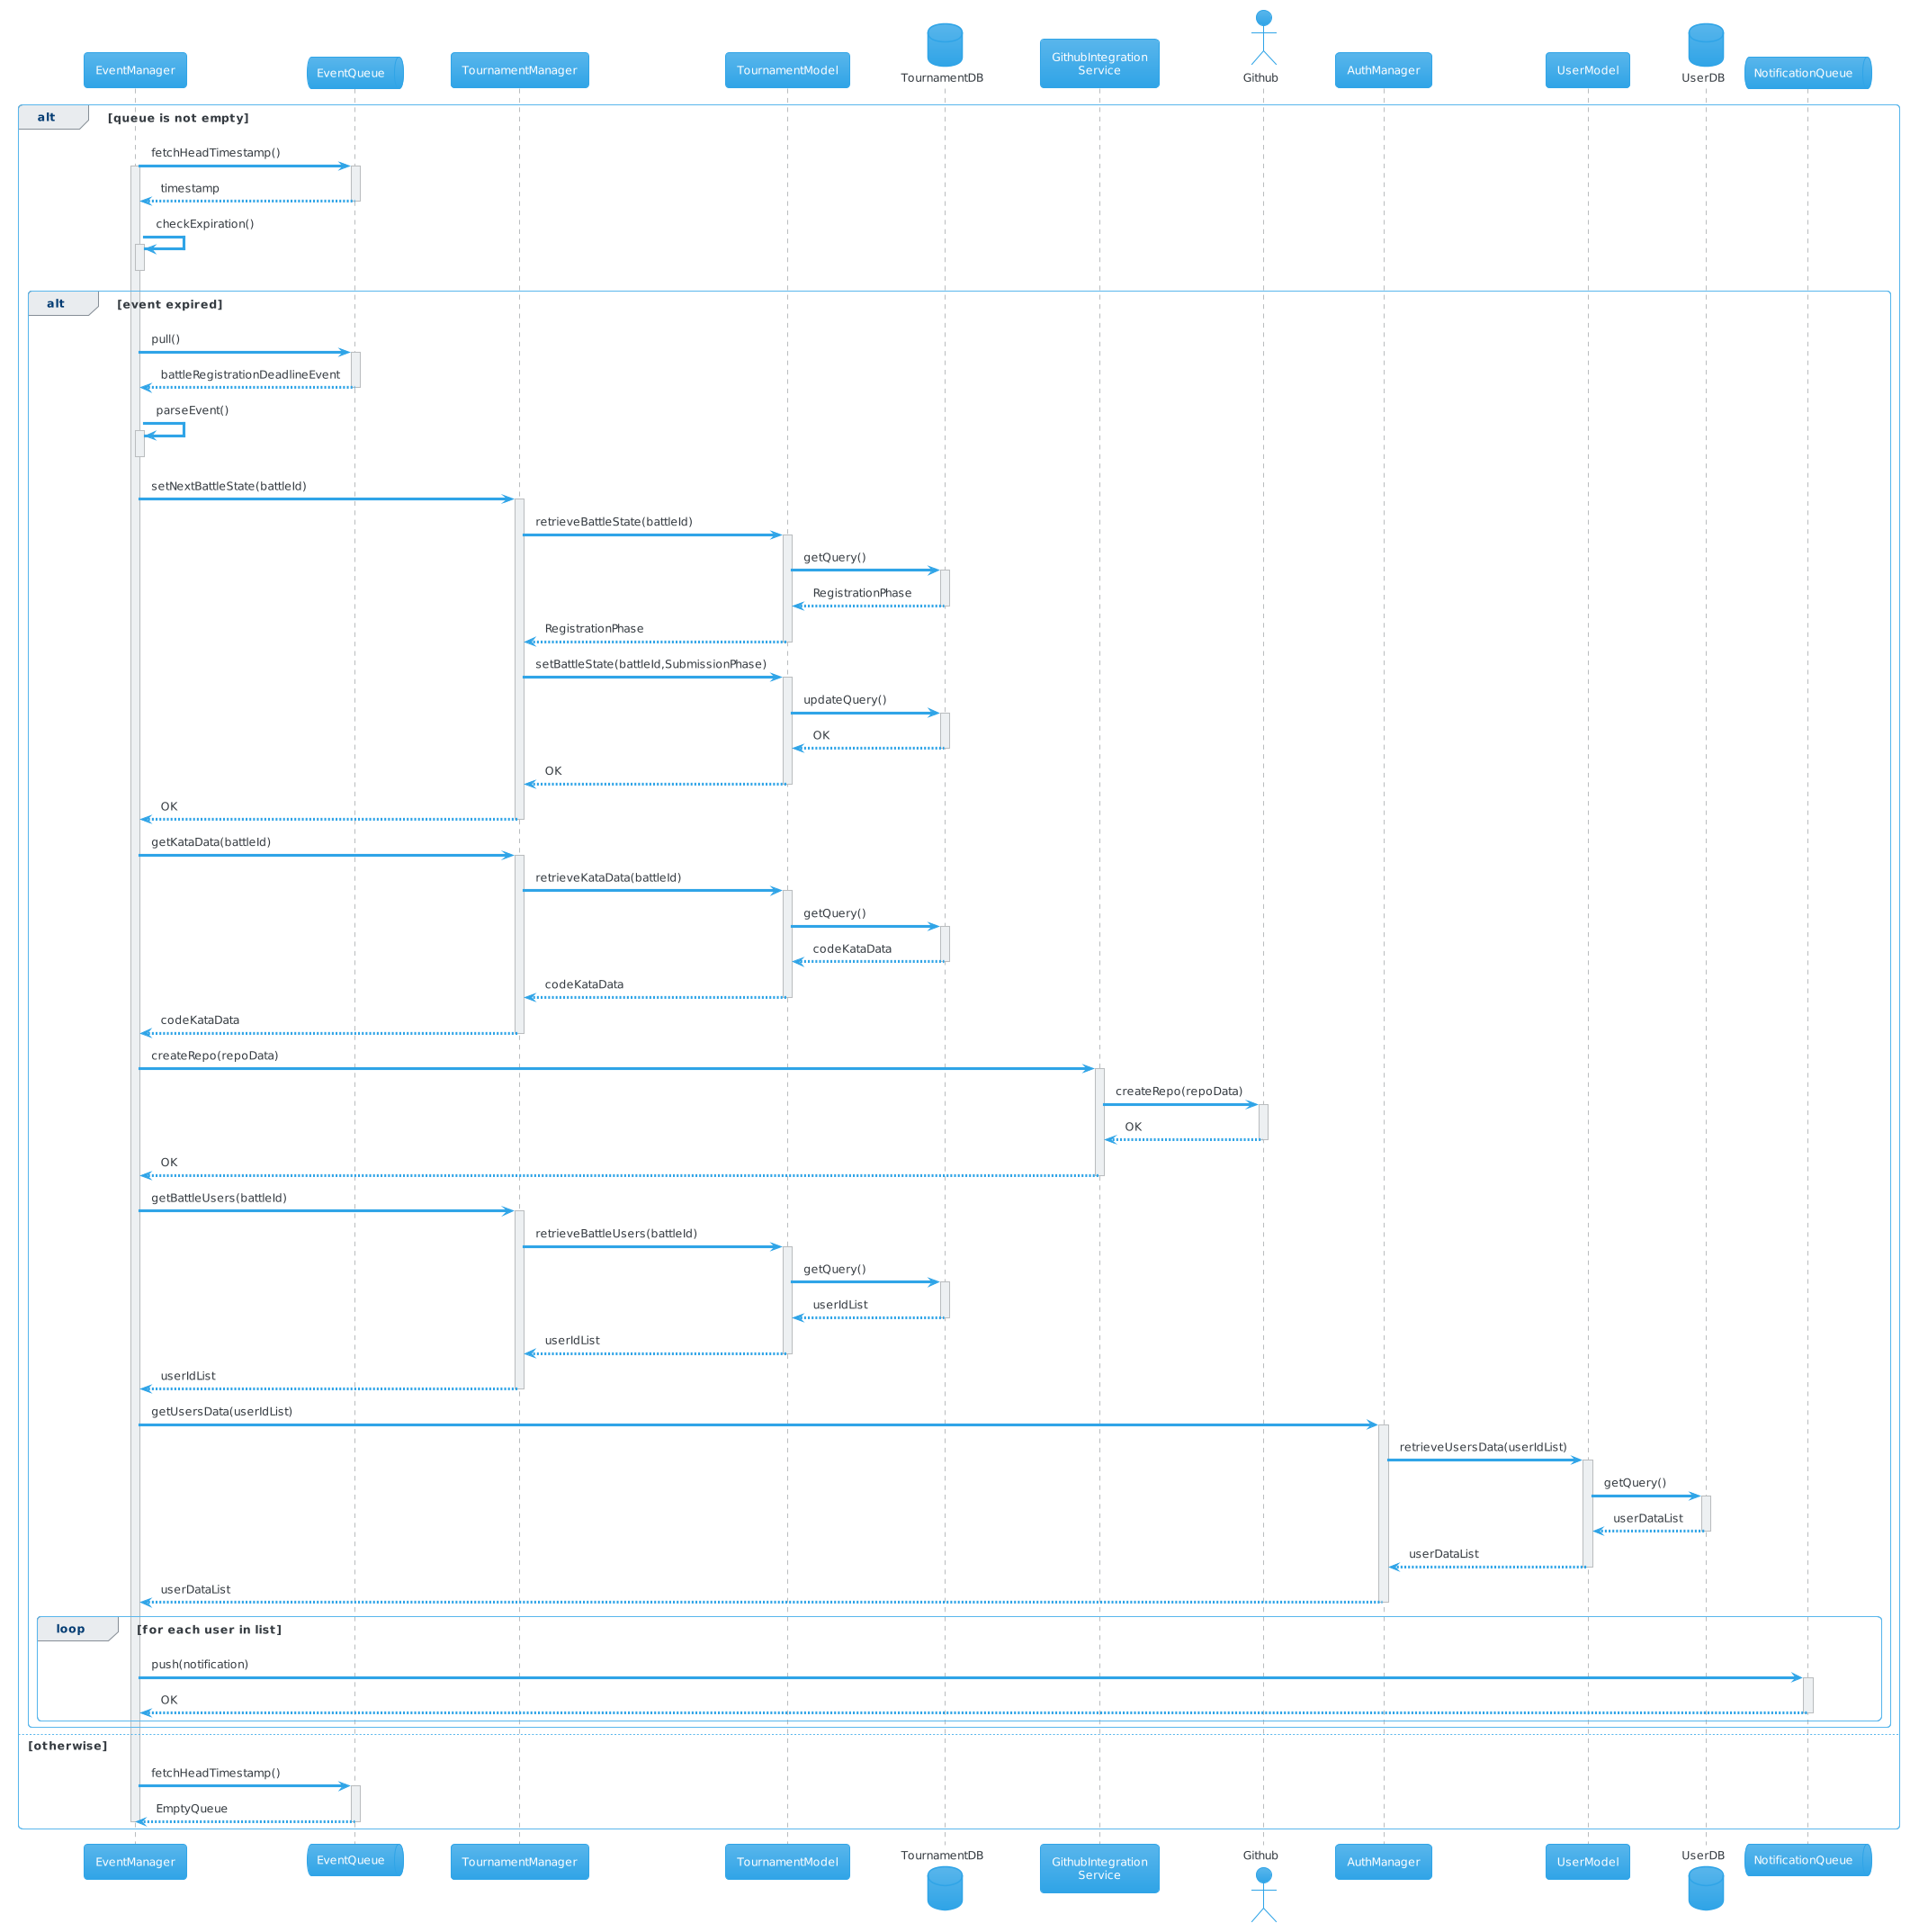
\includegraphics[width=1.2\textwidth]{Diagrams/sequence/create_battle_pull_deadline_registration.png}
    \caption{Pull of the deadline event, representing the end of the registration phase, generated by the battle creation}
\end{figure}
\begin{figure}[H]
    \hspace{0.6cm}
    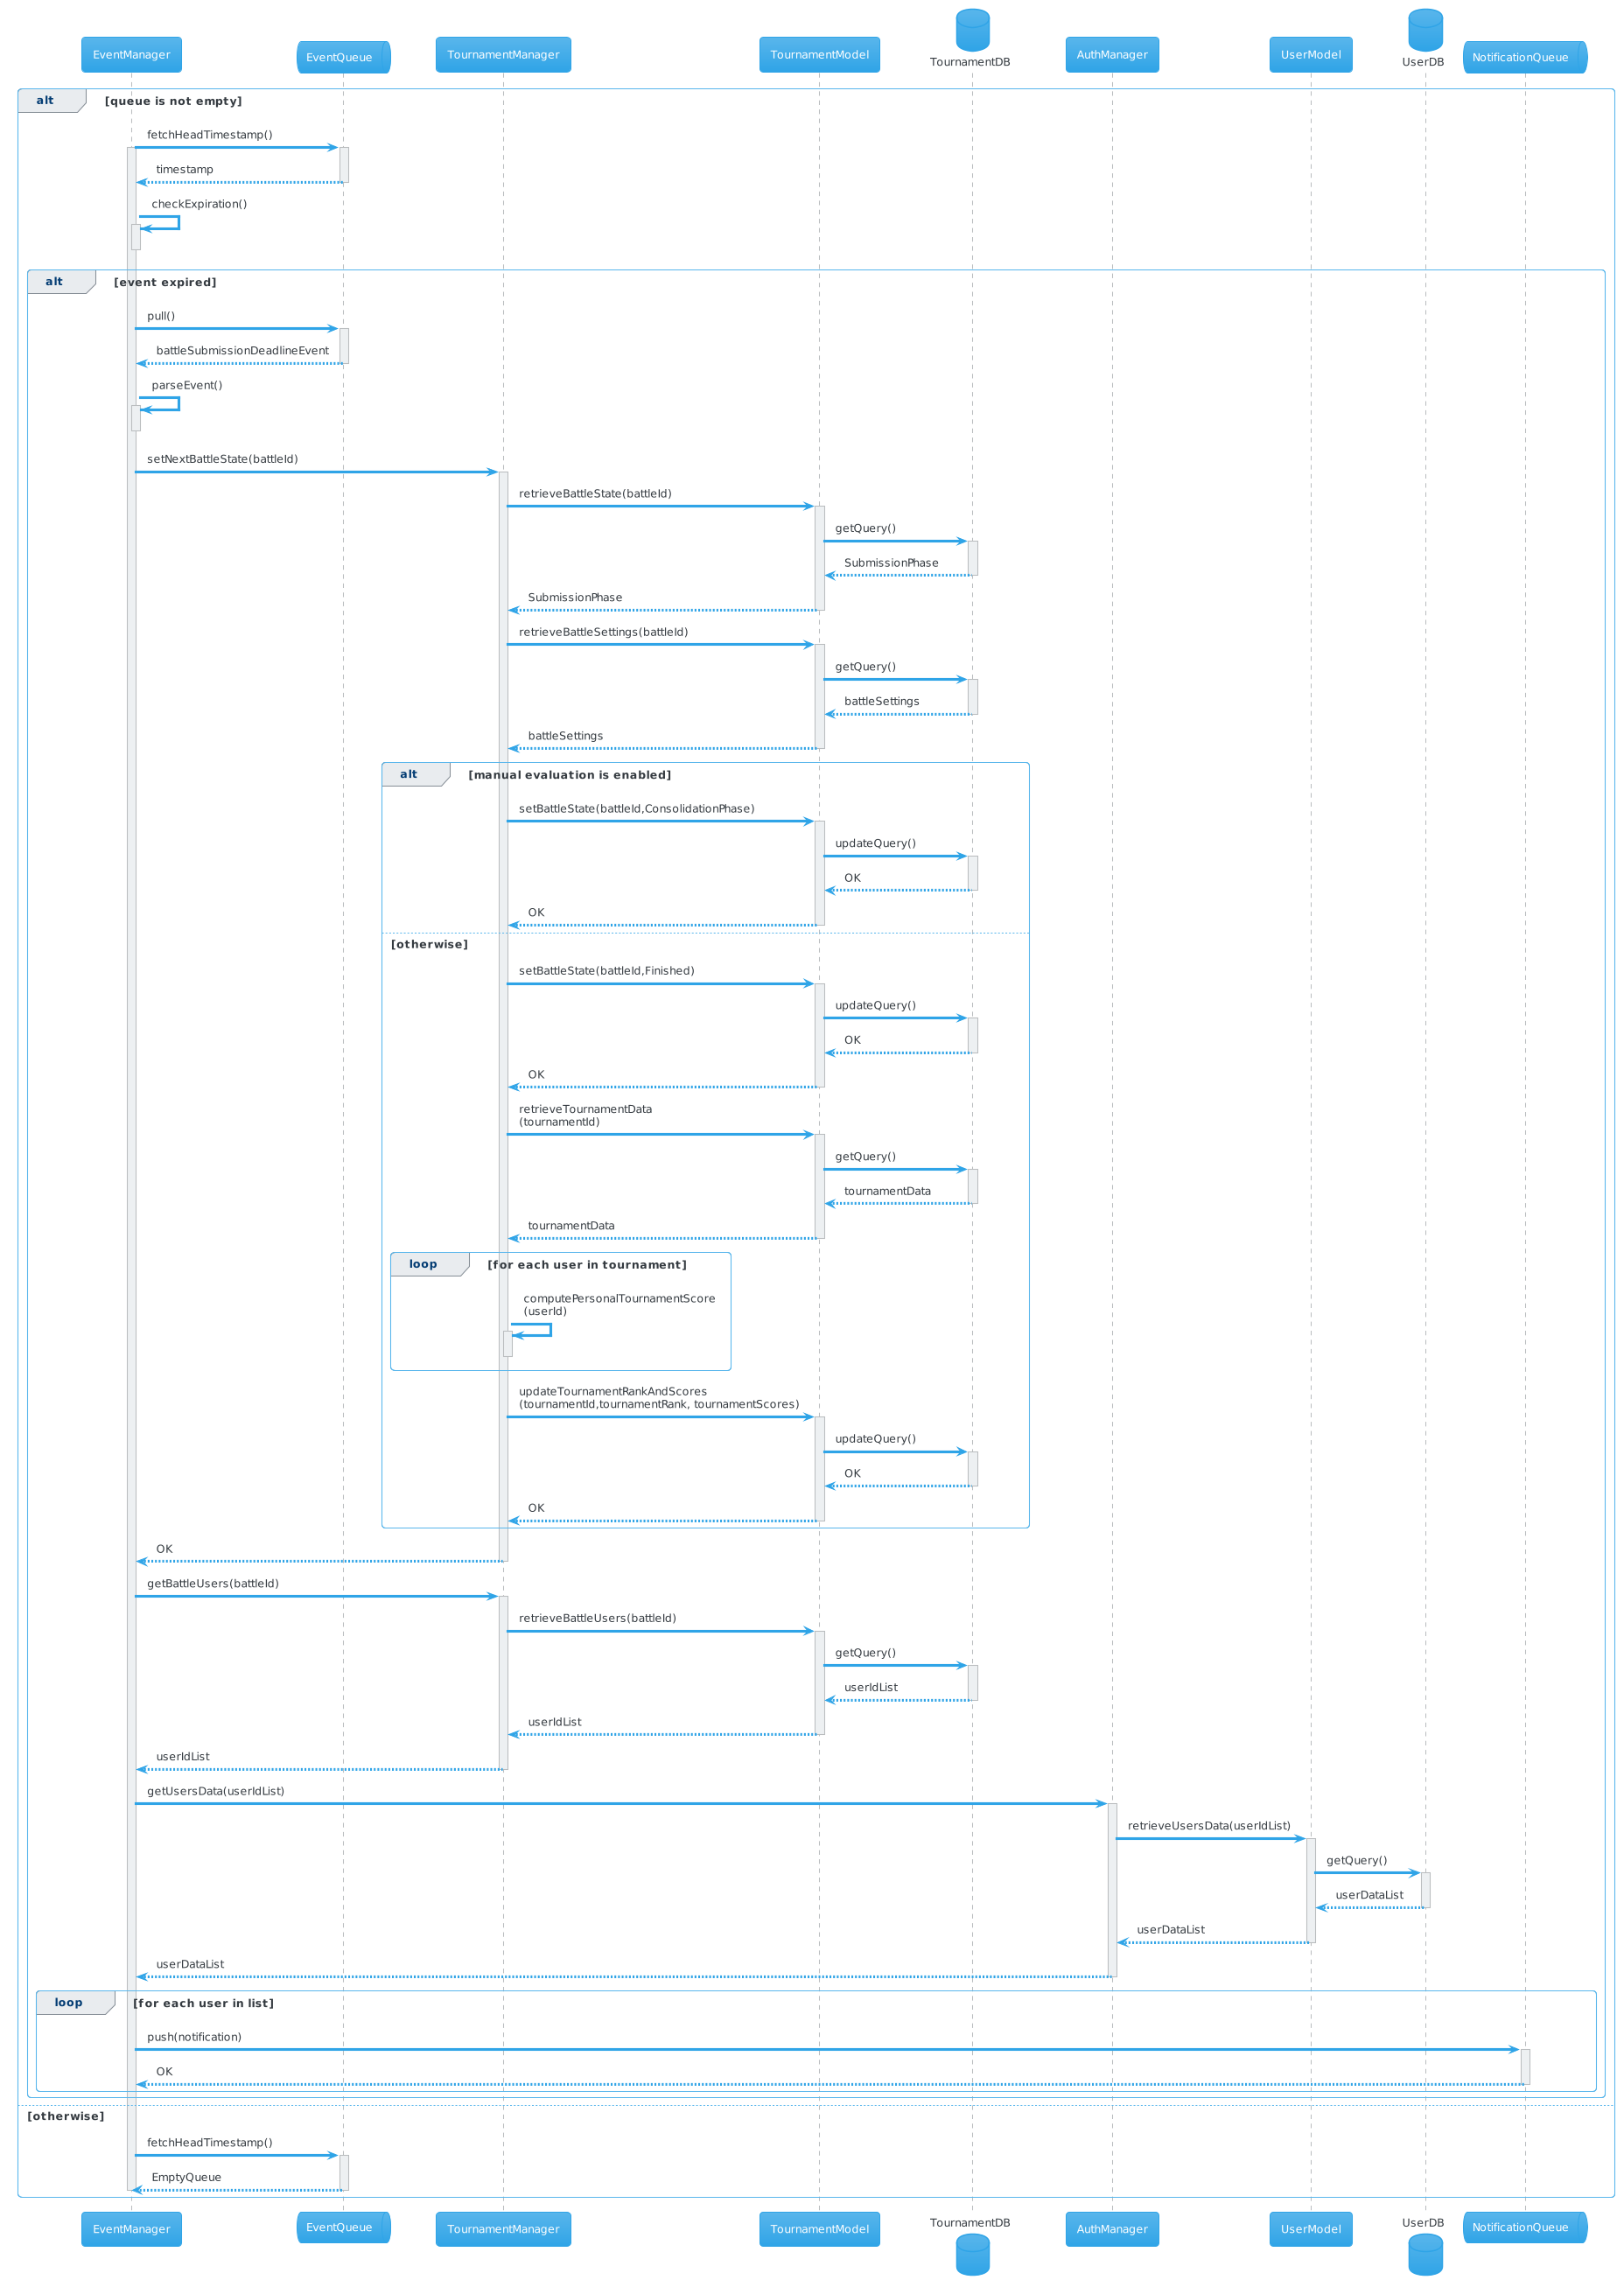
\includegraphics[width=0.9\textwidth]{Diagrams/sequence/create_battle_pull_deadline_submission.png}
    \caption{Pull of the deadline event, representing the end of the submission phase, generated by the battle creation}
\end{figure}

\subsubsection{Create a team}
\begin{figure}[H]
    \hspace{-1.5cm}
    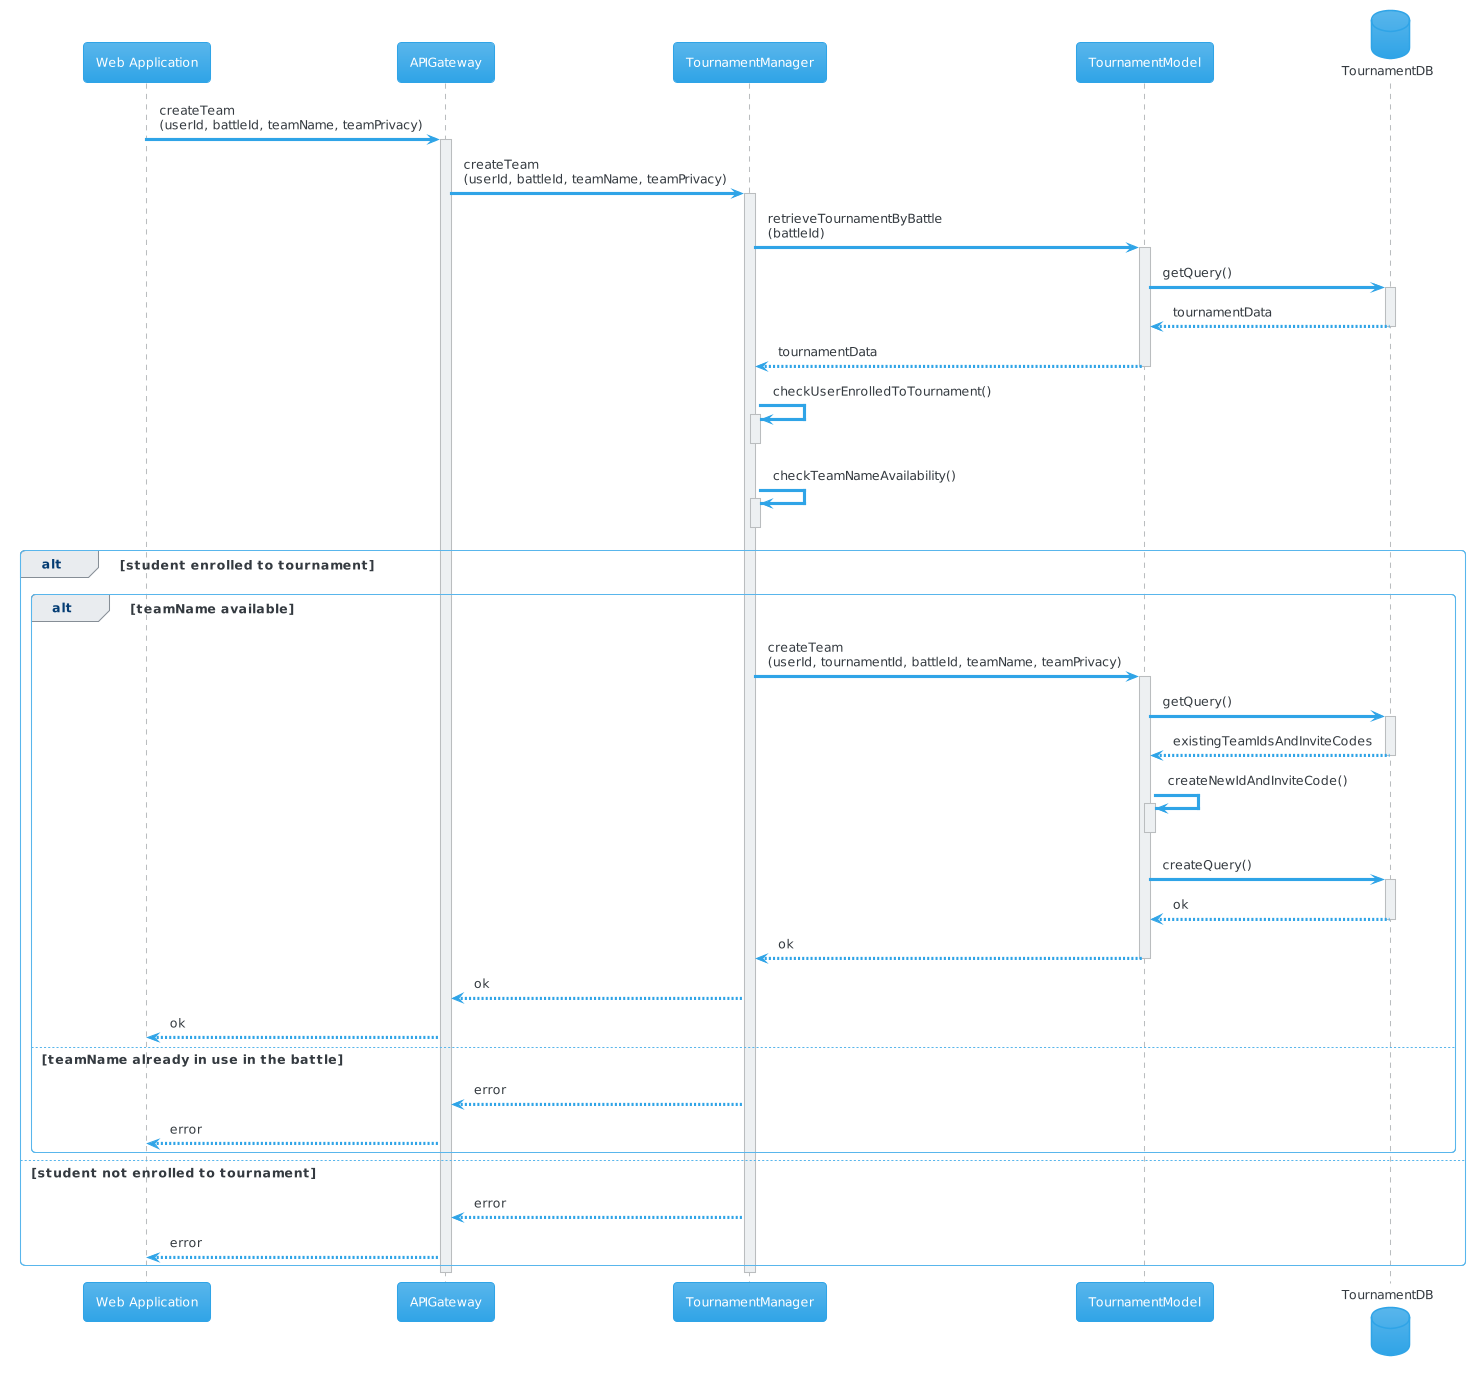
\includegraphics[width=1.2\textwidth]{Diagrams/sequence/create_team.png}
    \caption{Process of subscribing to a battle by creating a team}
\end{figure}

\subsubsection{Join a team}
\begin{figure}[H]
    \hspace{-0.7cm}
    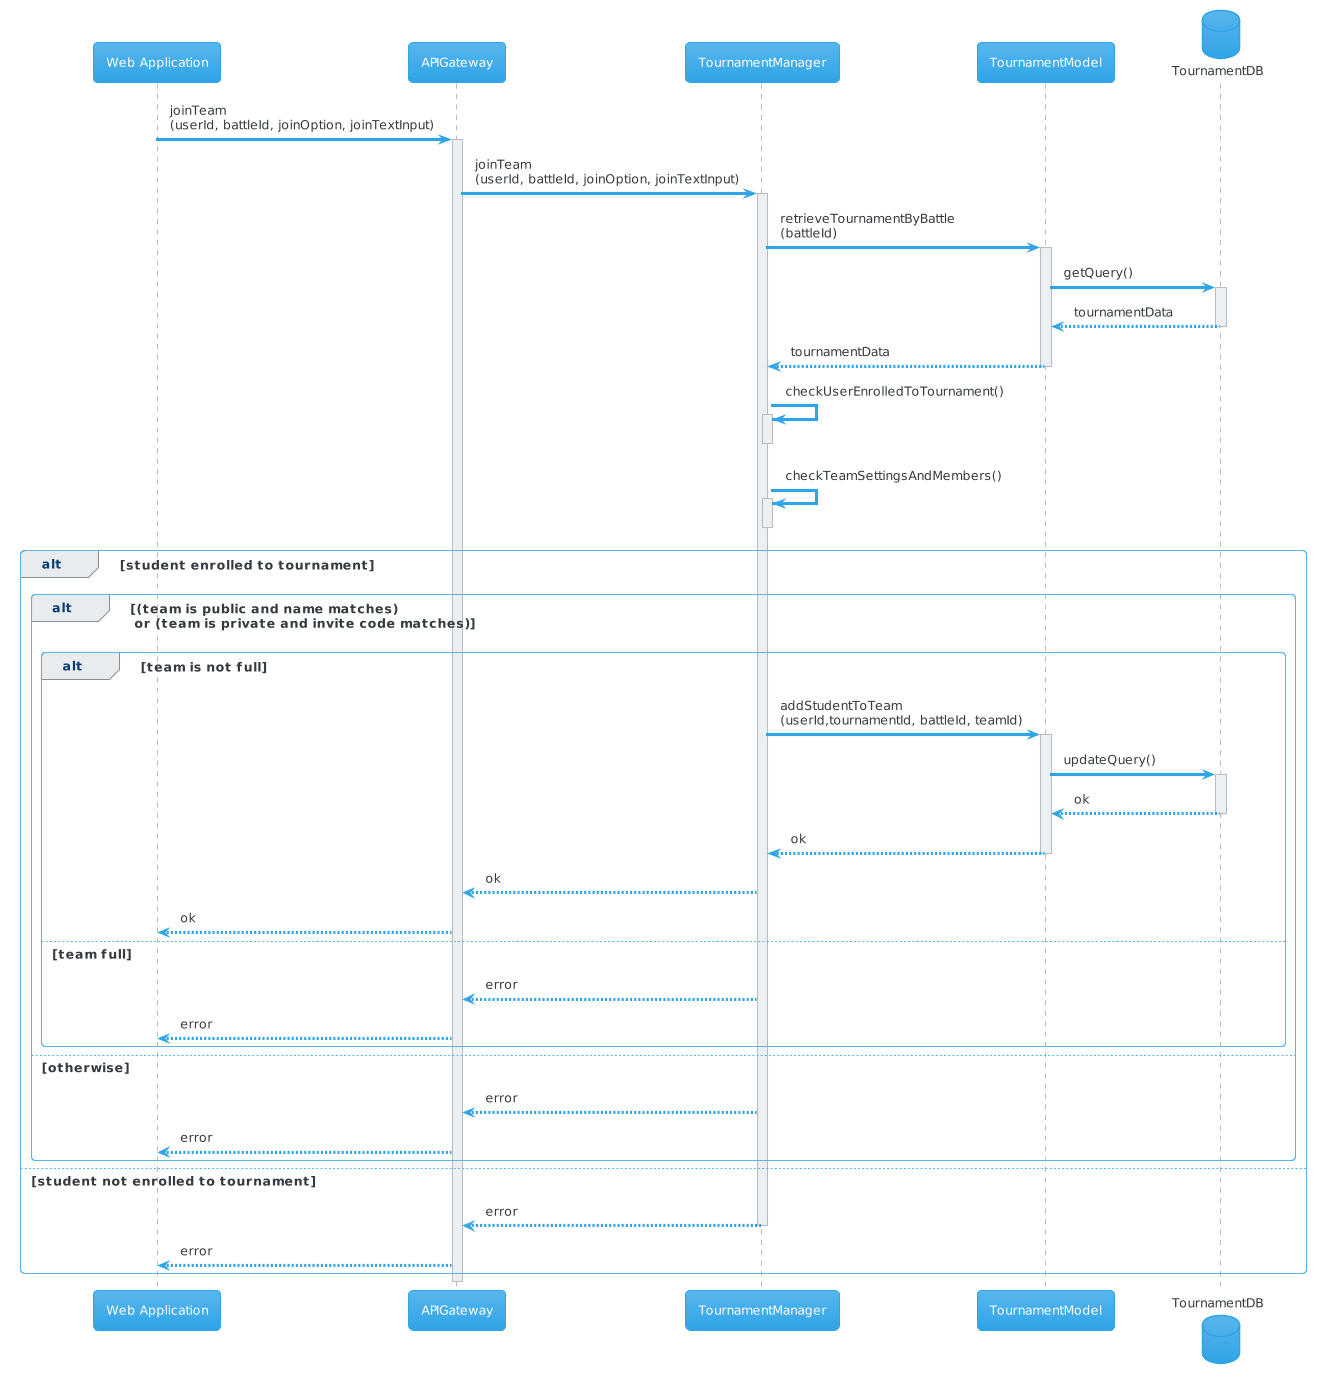
\includegraphics[width=1.1\textwidth]{Diagrams/sequence/join_team.png}
    \caption{Process of subscribing to a battle by joining an already existing team}
\end{figure}

\subsubsection{Configure team settings}
\begin{figure}[H]
    \hspace{-0.7cm}
    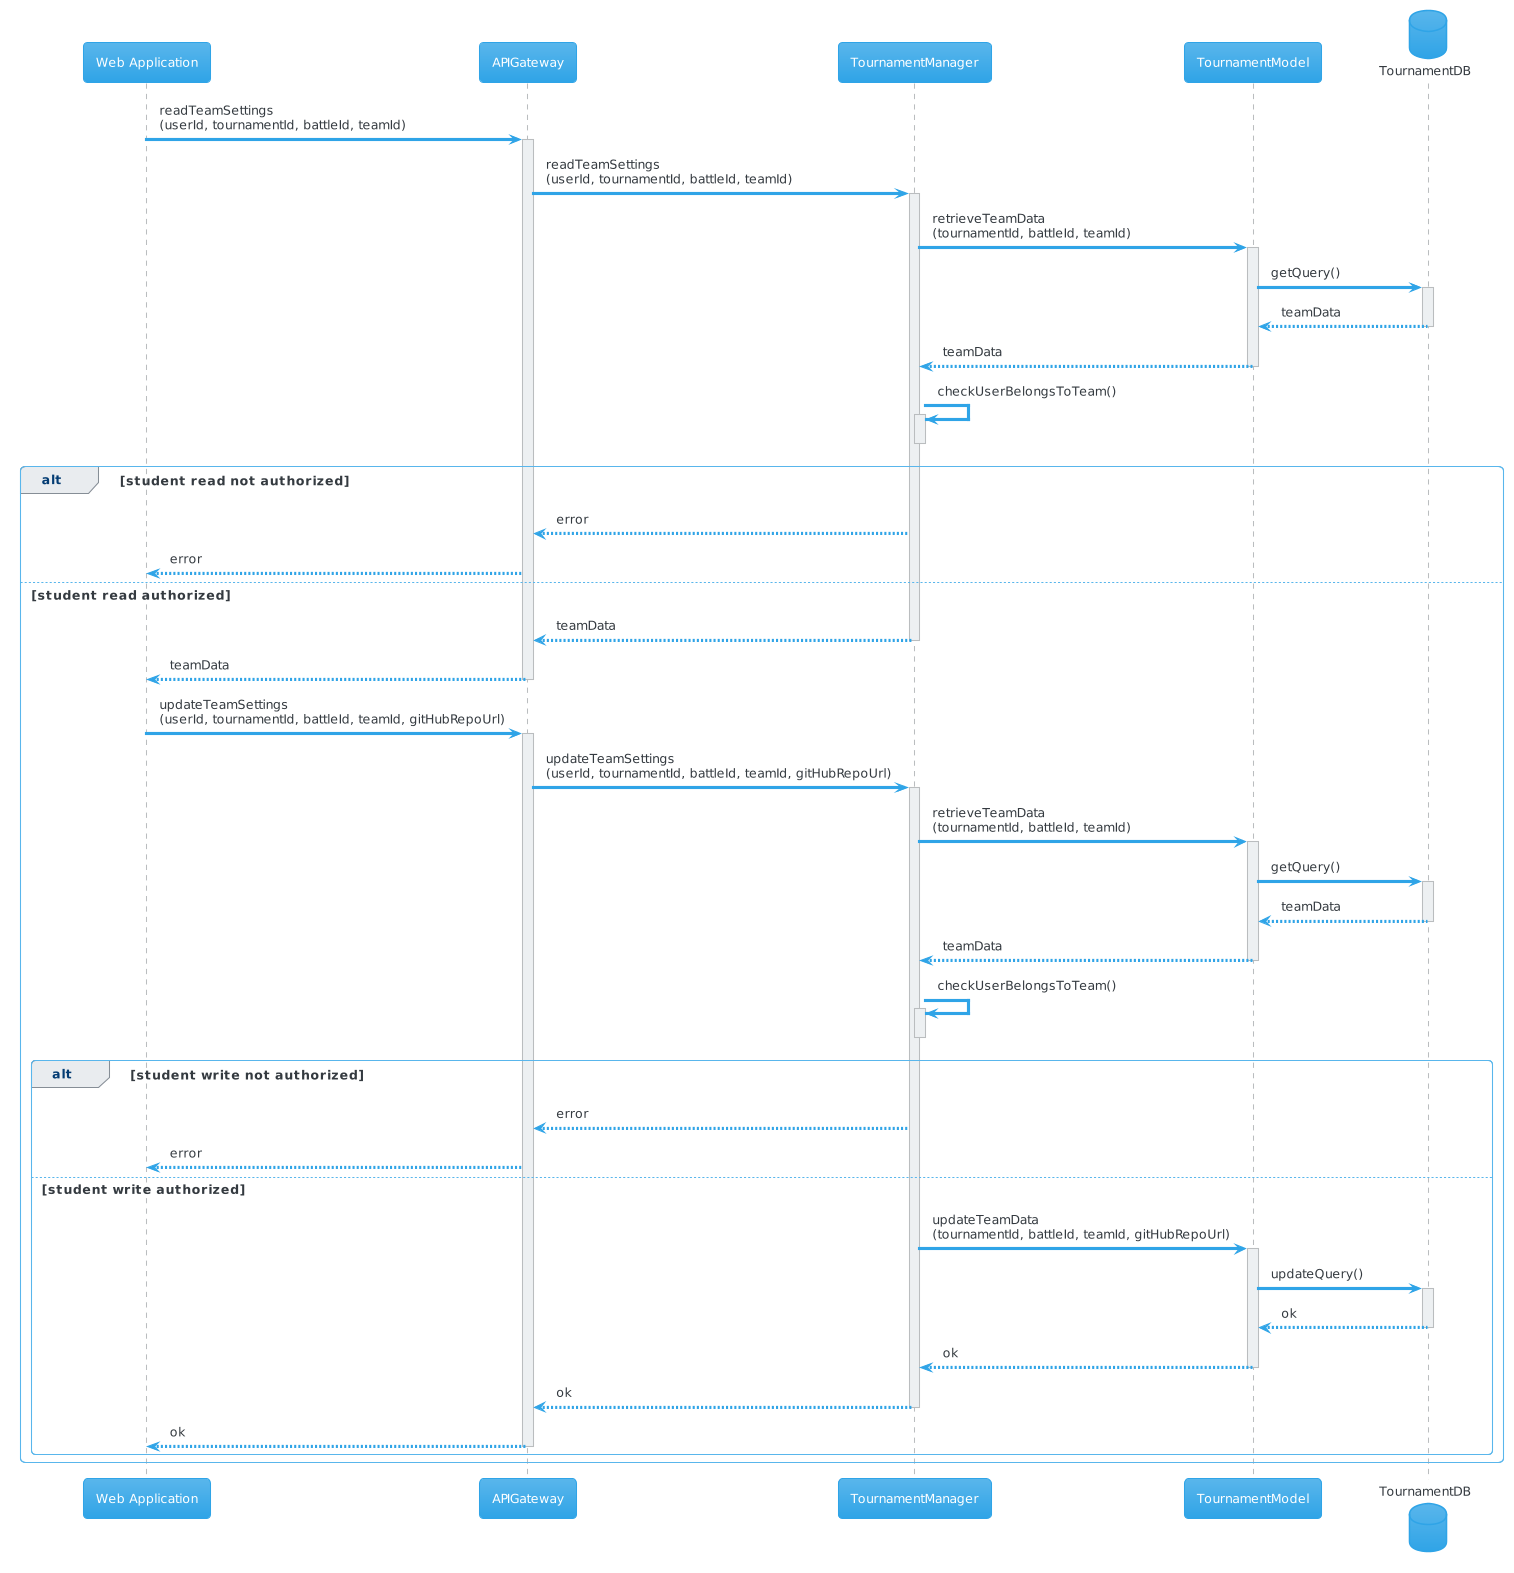
\includegraphics[width=1.1\textwidth]{Diagrams/sequence/configure_team_settings.png}
    \caption{Team settings configuration process}
\end{figure}

\subsubsection{Push of a new submission}
This scenario refers to the case in which a team pushes a new submission to its GitHub repository. The event is detected by GitHub Action, which notifies the system through the REST API exposed by the API Gateway. Is important to note that, just to be consistent with the RASD, the notification is represented in the diagram as a push on a queue of the relative teamId, while in reality it should push the API token that is univocally associated with the team sending the submission.
\begin{figure}[H]
    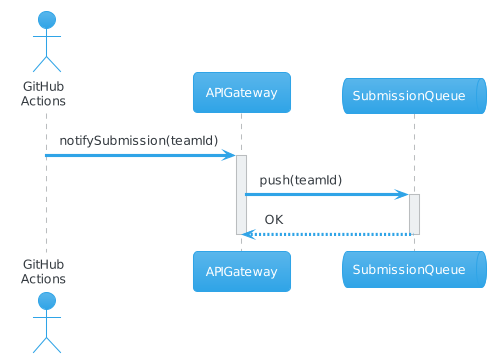
\includegraphics[width=1\textwidth]{Diagrams/sequence/new_submission.png}
    \caption{Reception of a new submission}
\end{figure}

\newpage
\subsubsection{Evaluation of a submission}
\begin{figure}[H]
    \hspace{0.5cm}
    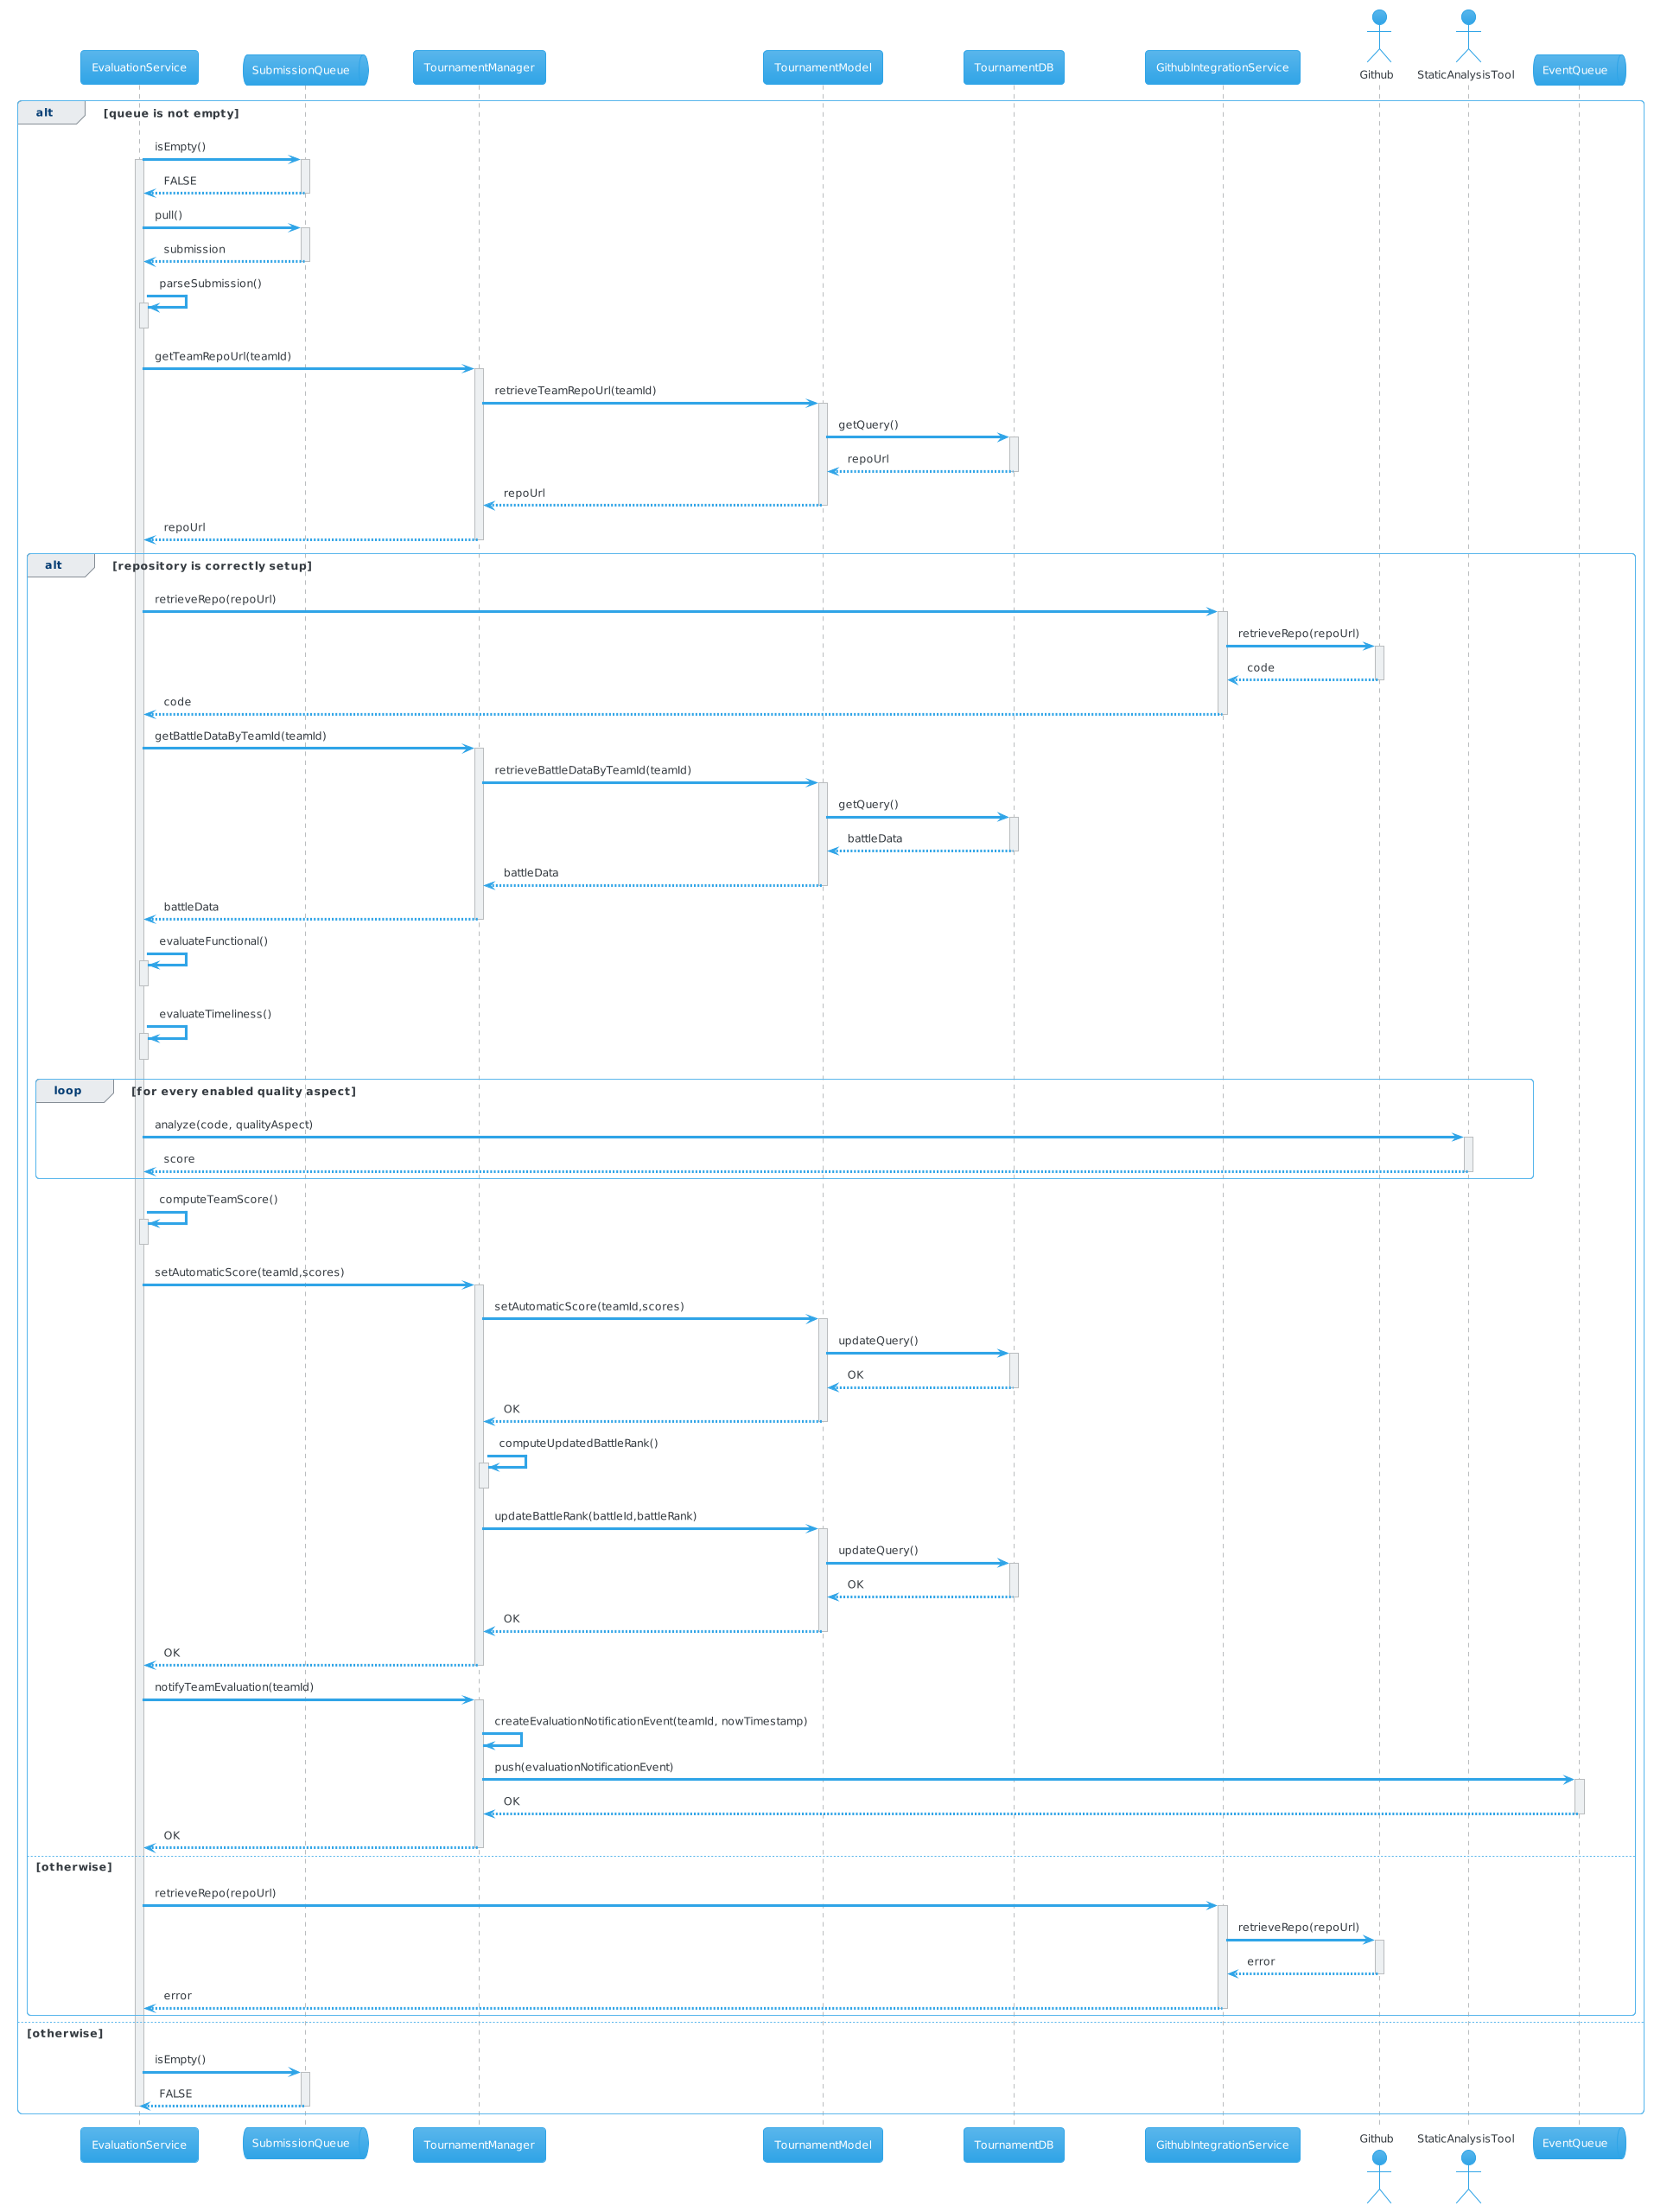
\includegraphics[width=0.9\textwidth]{Diagrams/sequence/evaluate_submission.png}
    \caption{Submission evaluation process}
\end{figure}
\begin{figure}[H]
    \hspace{-1.5cm}
    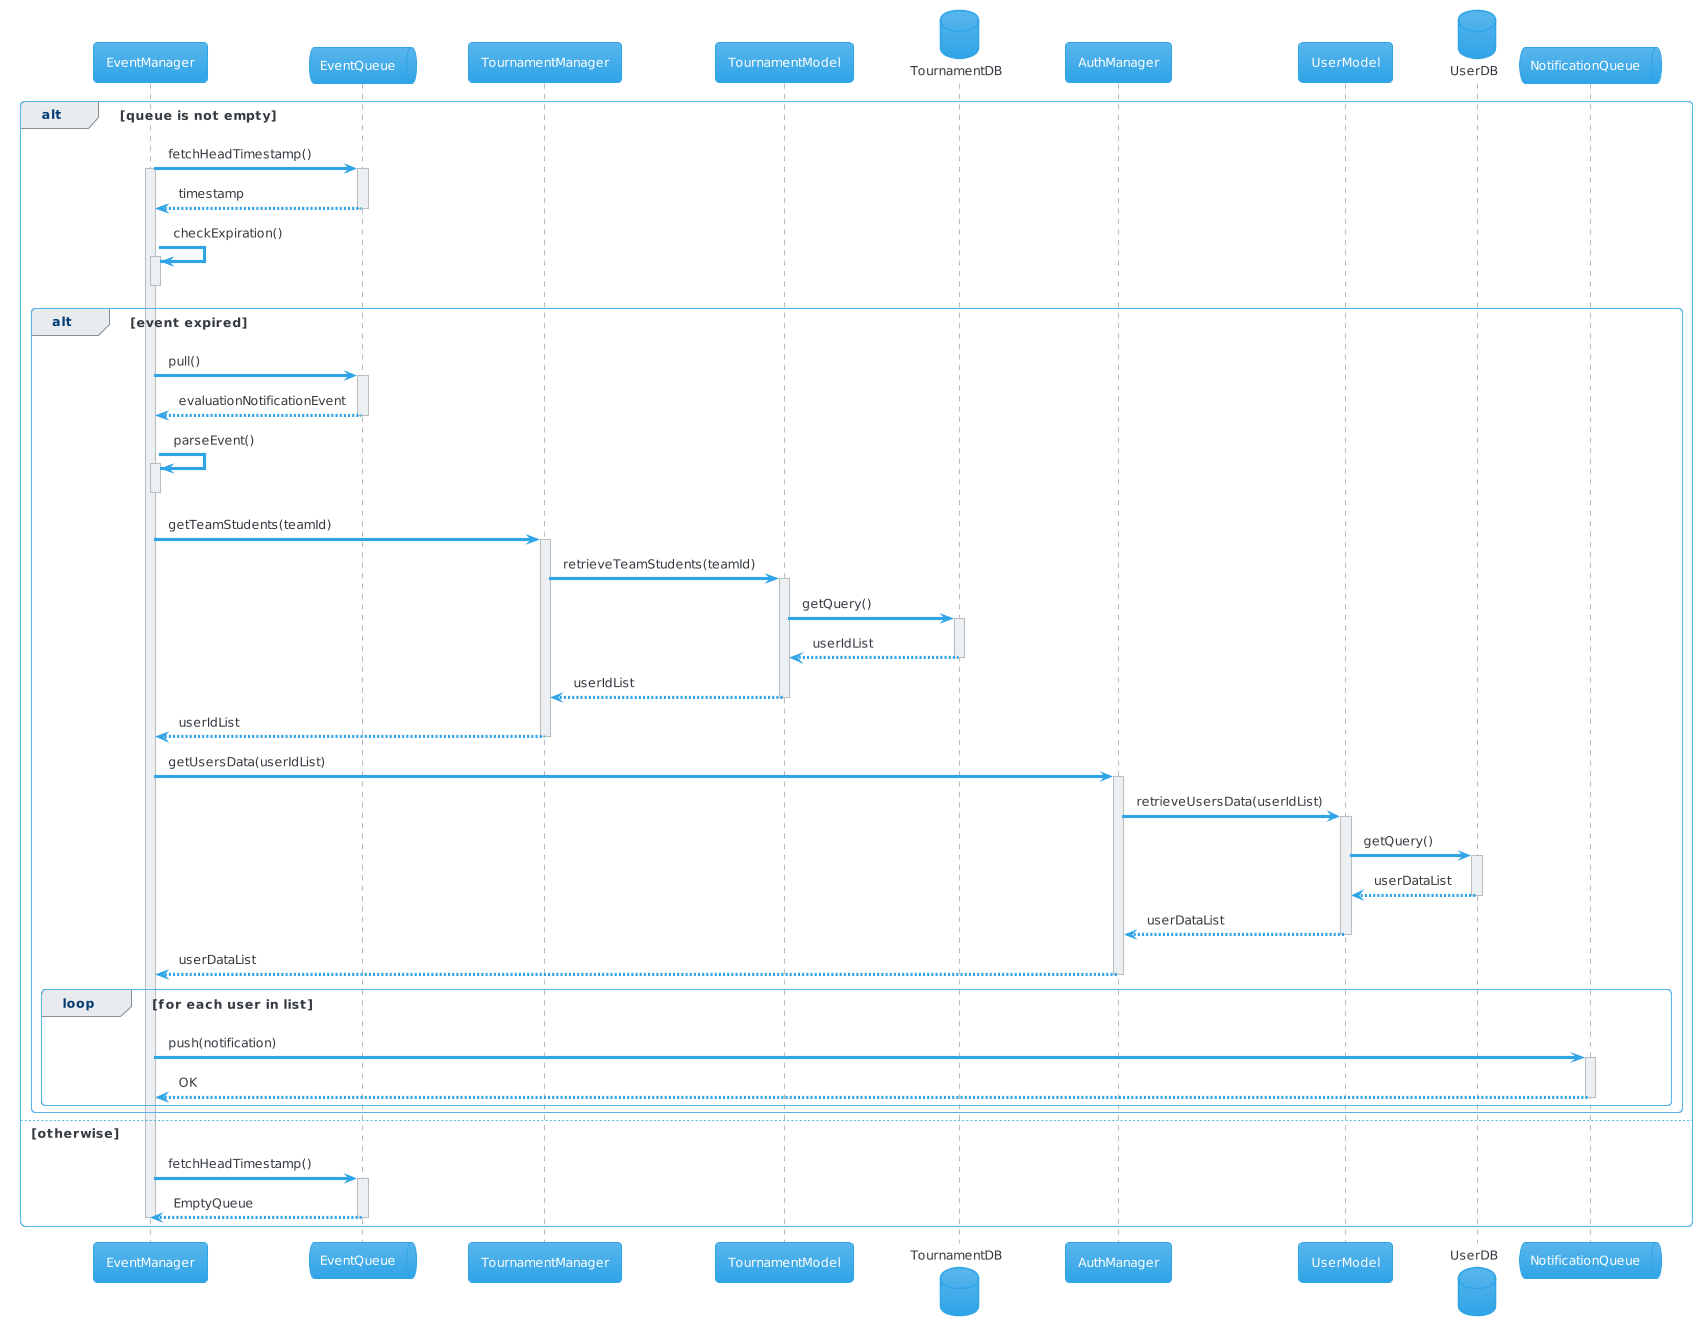
\includegraphics[width=1.2\textwidth]{Diagrams/sequence/evaluate_submission_pull_notification.png}
    \caption{Pull of the notification event generated by the evaluation of a submission}
\end{figure}

\newpage
\subsubsection{Manual evaluation}
\begin{figure}[H]
    \hspace{-1.5cm}
    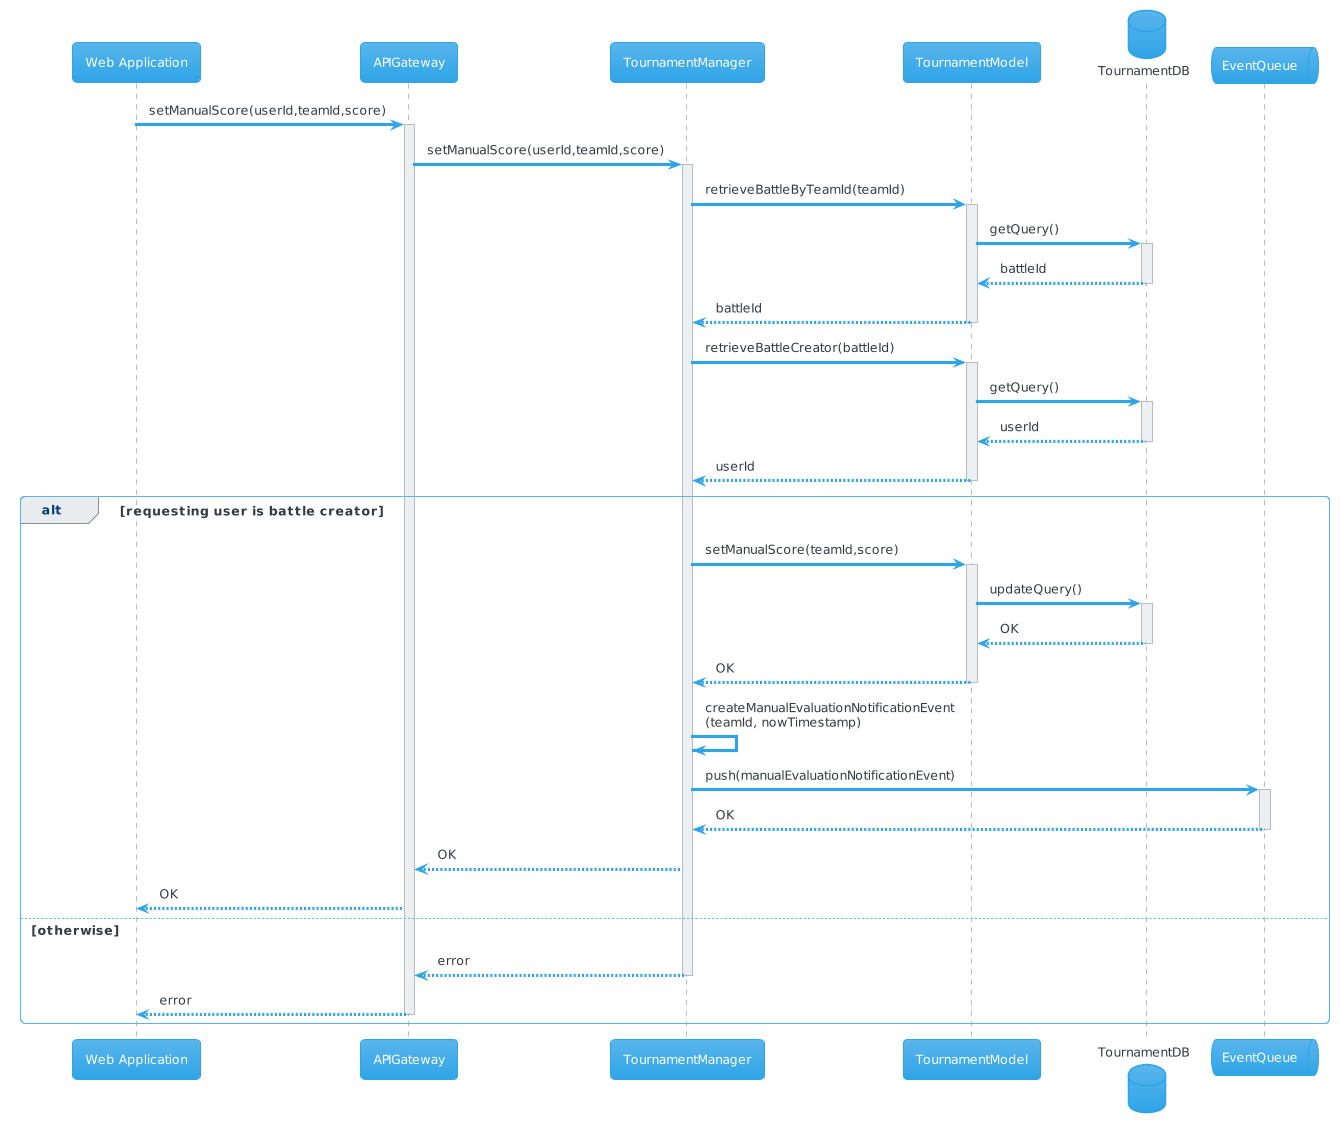
\includegraphics[width=1.2\textwidth]{Diagrams/sequence/manual_evaluate_submission.png}
    \caption{Manual evaluation process}
\end{figure}
Also in this case the pull of the notification has not been represented since it would be identical to the one shown in the previous scenario.

\subsubsection{Visualization of a submission' score}
\begin{figure}[H]
    \hspace{-1.5cm}
    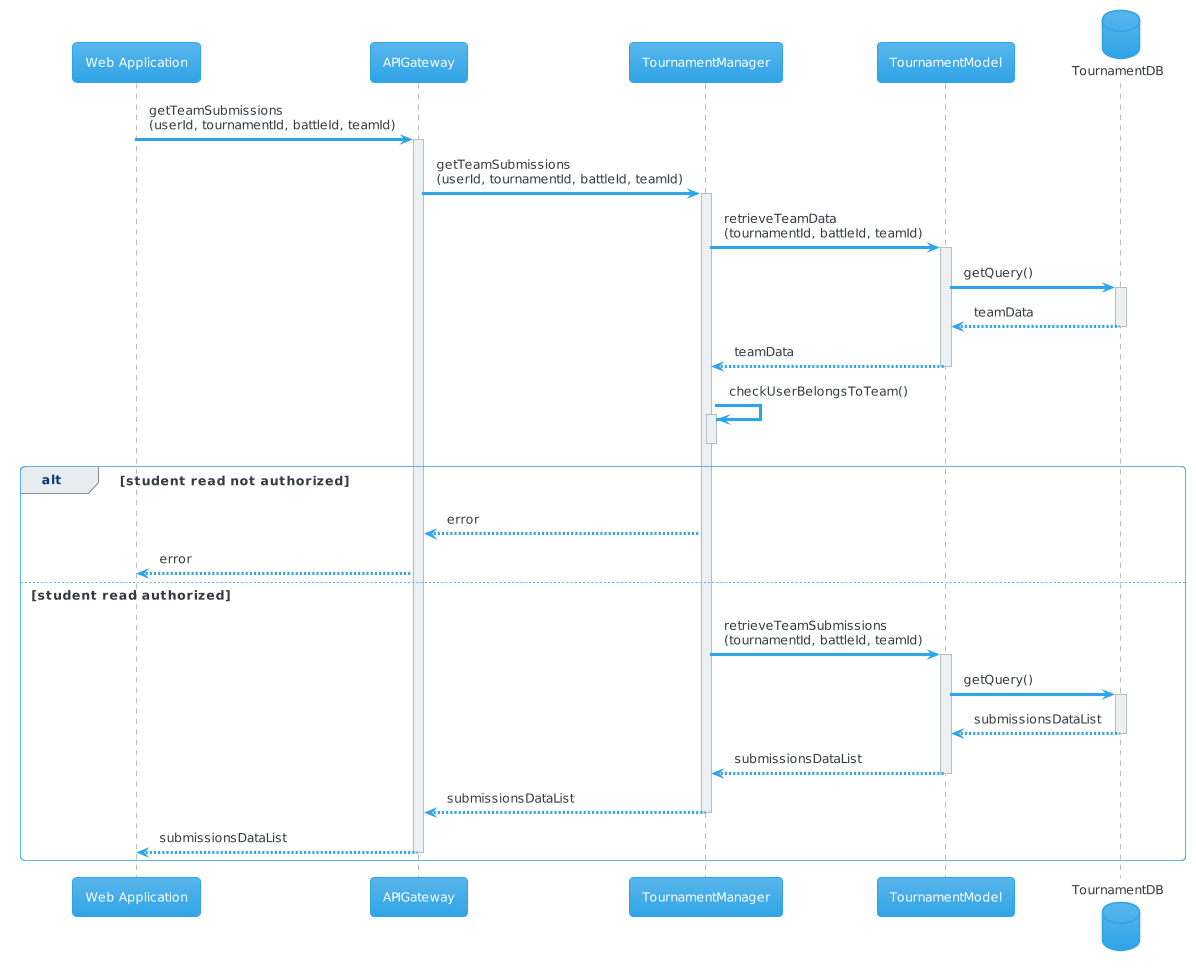
\includegraphics[width=1.2\textwidth]{Diagrams/sequence/visualize_score.png}
    \caption{Score visualization process}
\end{figure}

\newpage
\subsubsection{Visualization of a ranking}
\begin{figure}[H]
    \hspace{1cm}
    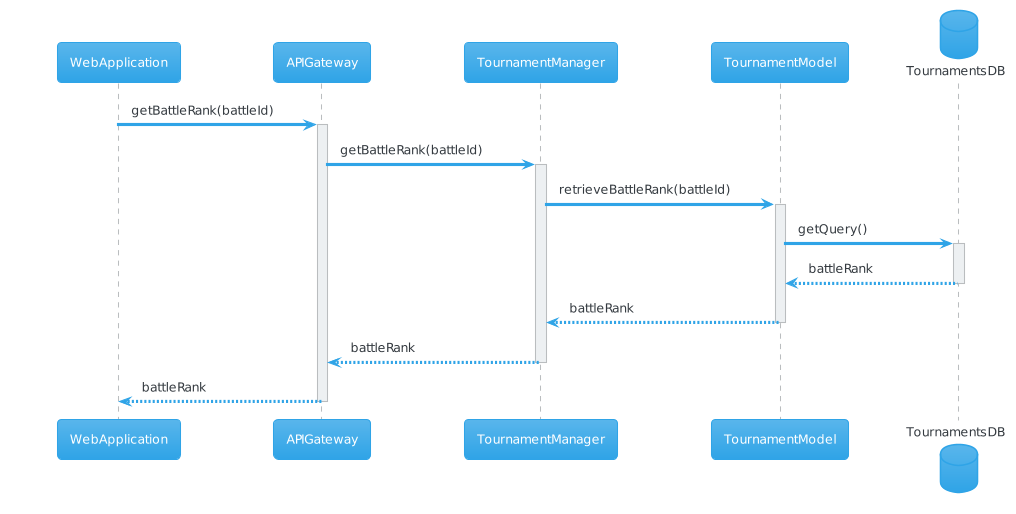
\includegraphics[width=0.8\textwidth]{Diagrams/sequence/visualize_battle_rank.png}
    \caption{Battle's rank visualization process}
\end{figure}
\begin{figure}[H]
    \hspace{1.2cm}
    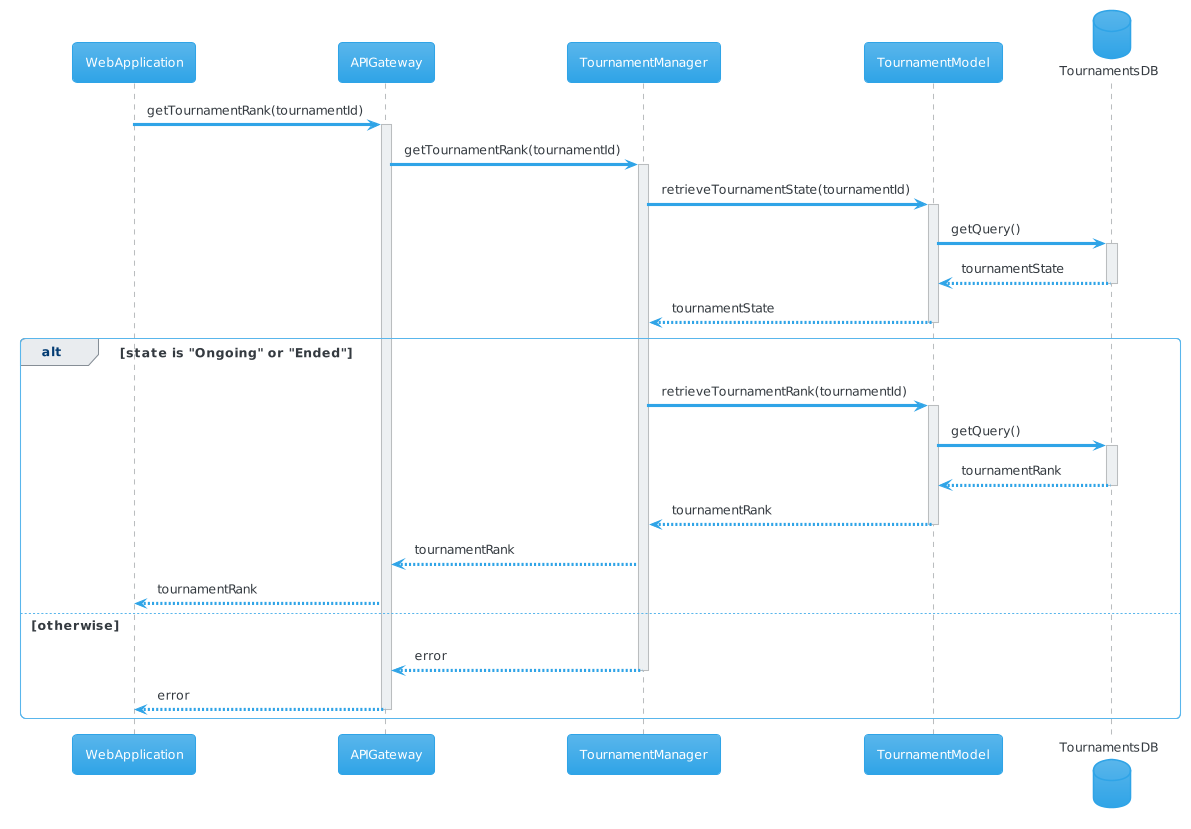
\includegraphics[width=0.8\textwidth]{Diagrams/sequence/visualize_tournament_rank.png}
    \caption{Tournament's rank visualization process}
\end{figure}

\subsubsection{Closure of a battle's consolidation phase}
This scenario is only available to the educator that created the battle and only if manual evaluation was enabled: in the other case a very similar sequence of events is triggered, with which the battle' state is automatically set to "Finished" after the submission phase deadline is reached and all the participating teams are notified, similarly to this case.
\begin{figure}[H]
    \hspace{-1.7cm}
    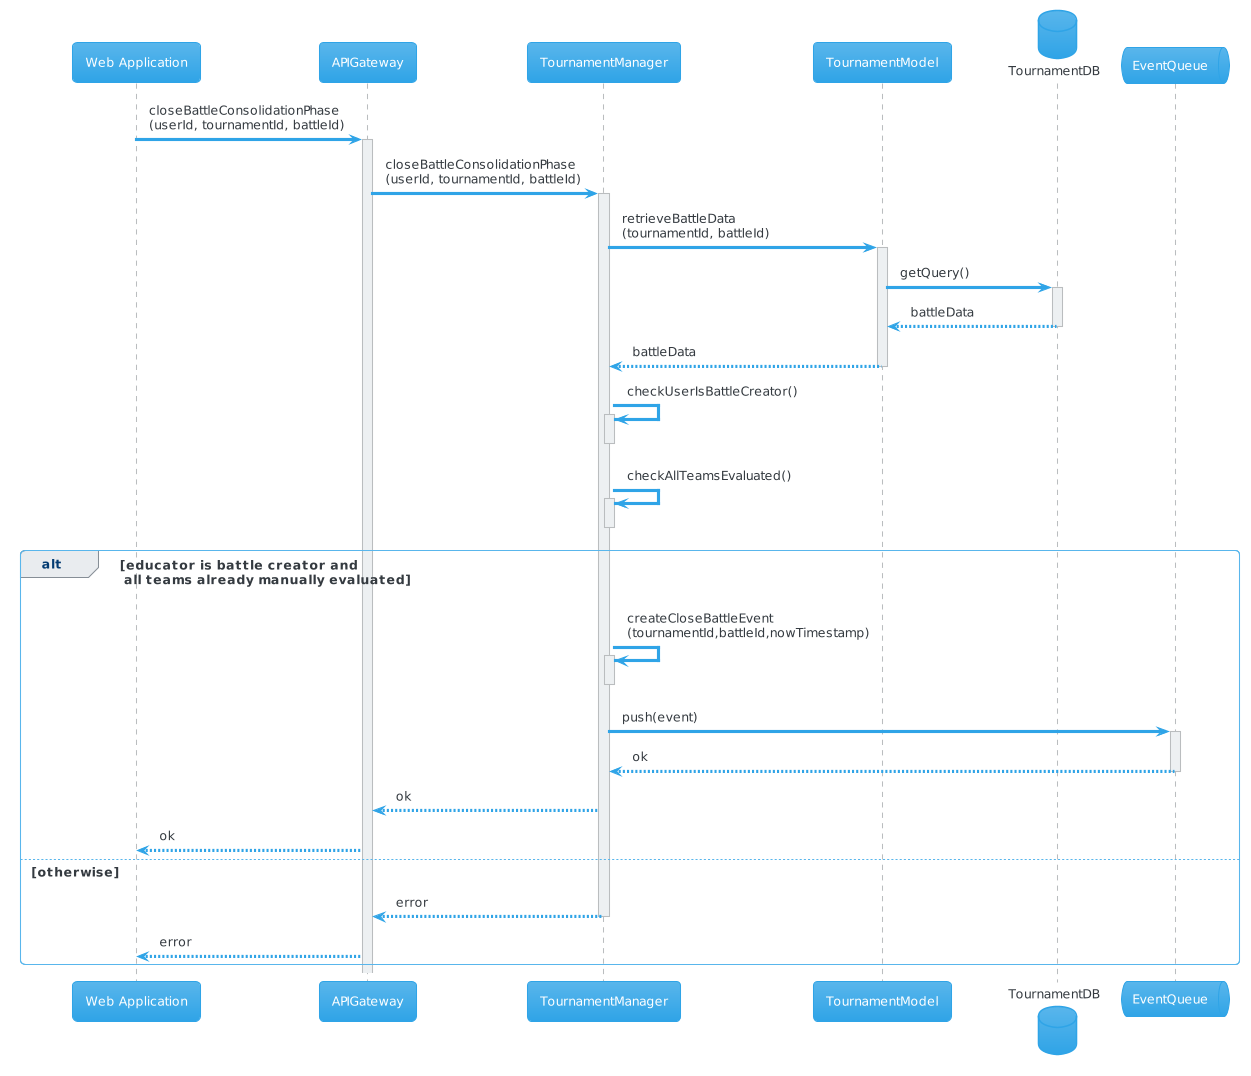
\includegraphics[width=1.2\textwidth]{Diagrams/sequence/close_battle.png}
    \caption{Process of manually ending the consolidation phase of a battle}
\end{figure}
\begin{figure}[H]
    \hspace{0.5cm}
    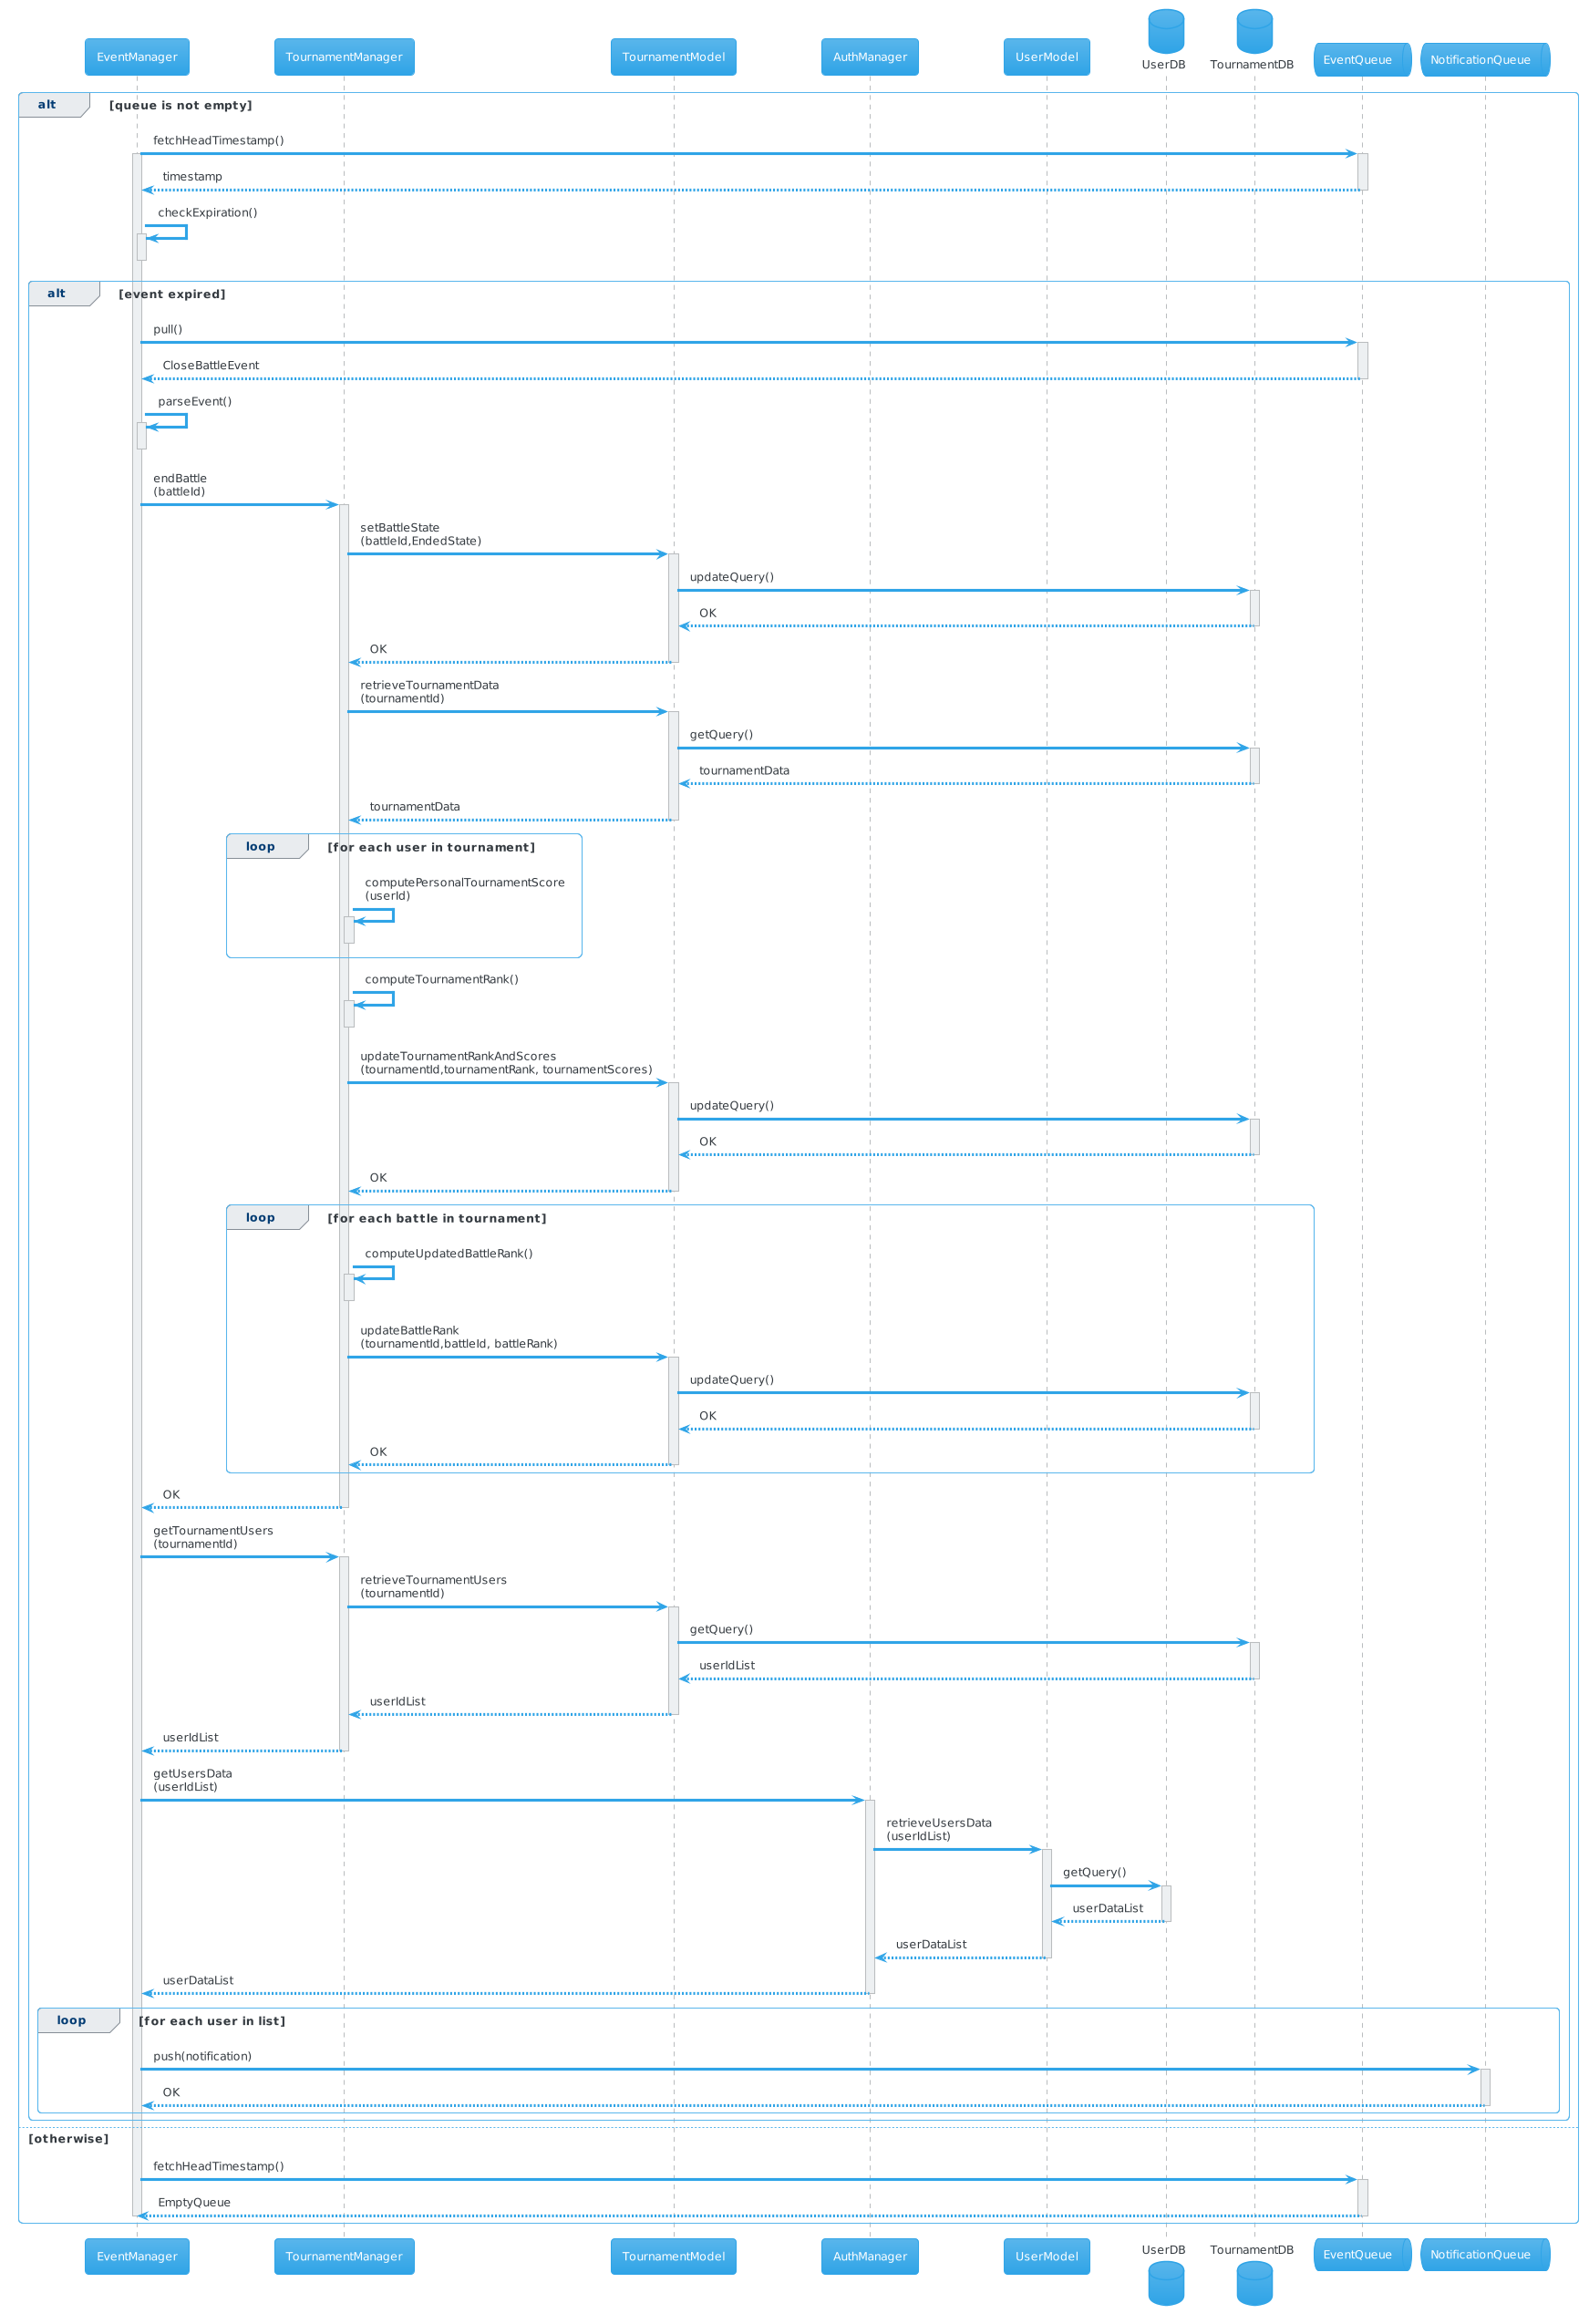
\includegraphics[width=0.9\textwidth]{Diagrams/sequence/close_battle_pull.png}
    \caption{Pull of the notification event generated by the end of a battle}
\end{figure}

\subsubsection{Closure of a tournament}
\begin{figure}[H]
    \hspace{-1.7cm}
    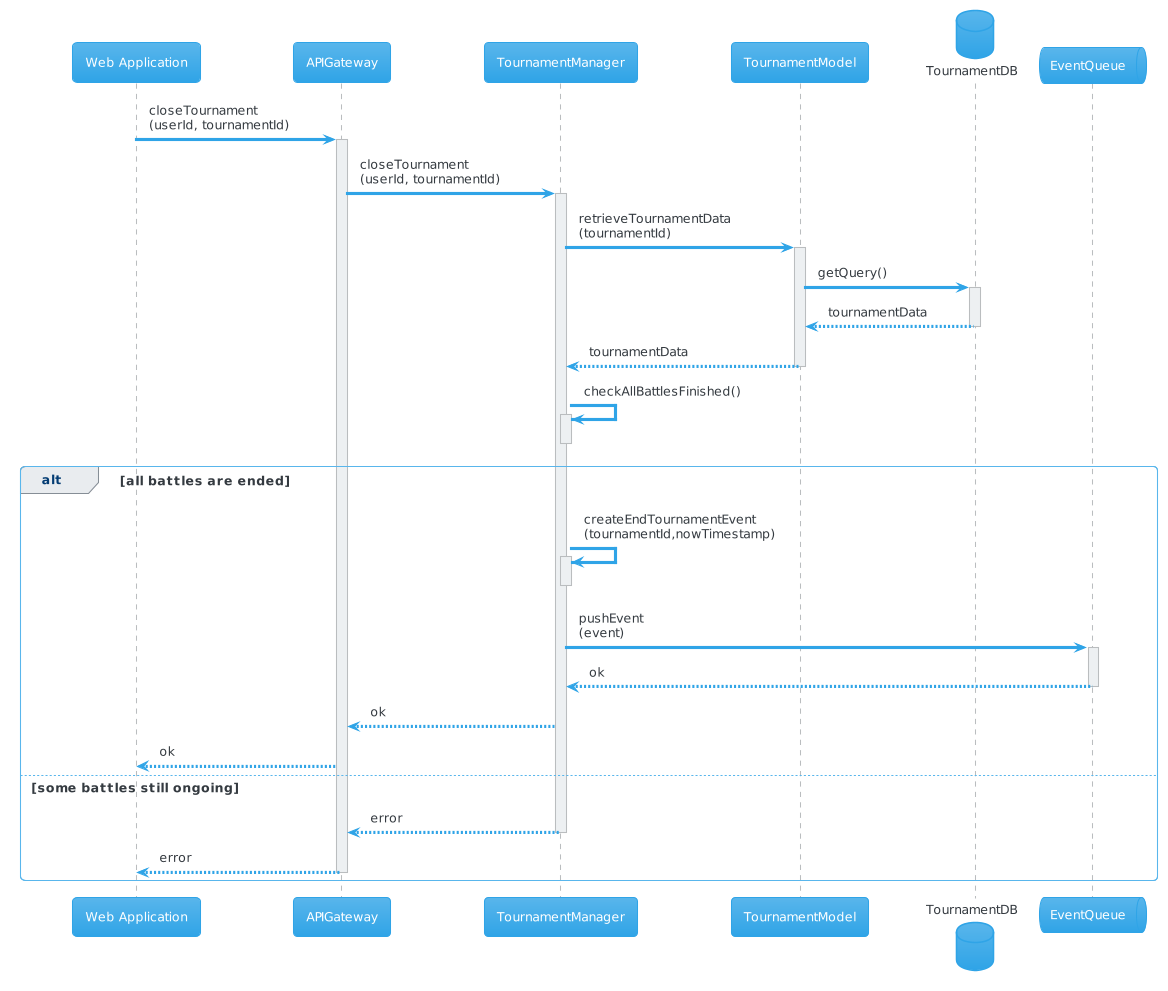
\includegraphics[width=1.2\textwidth]{Diagrams/sequence/close_tournament.png}
    \caption{Process of closing a tournament}
\end{figure}
\begin{figure}[H]
    \hspace{-1.5cm}
    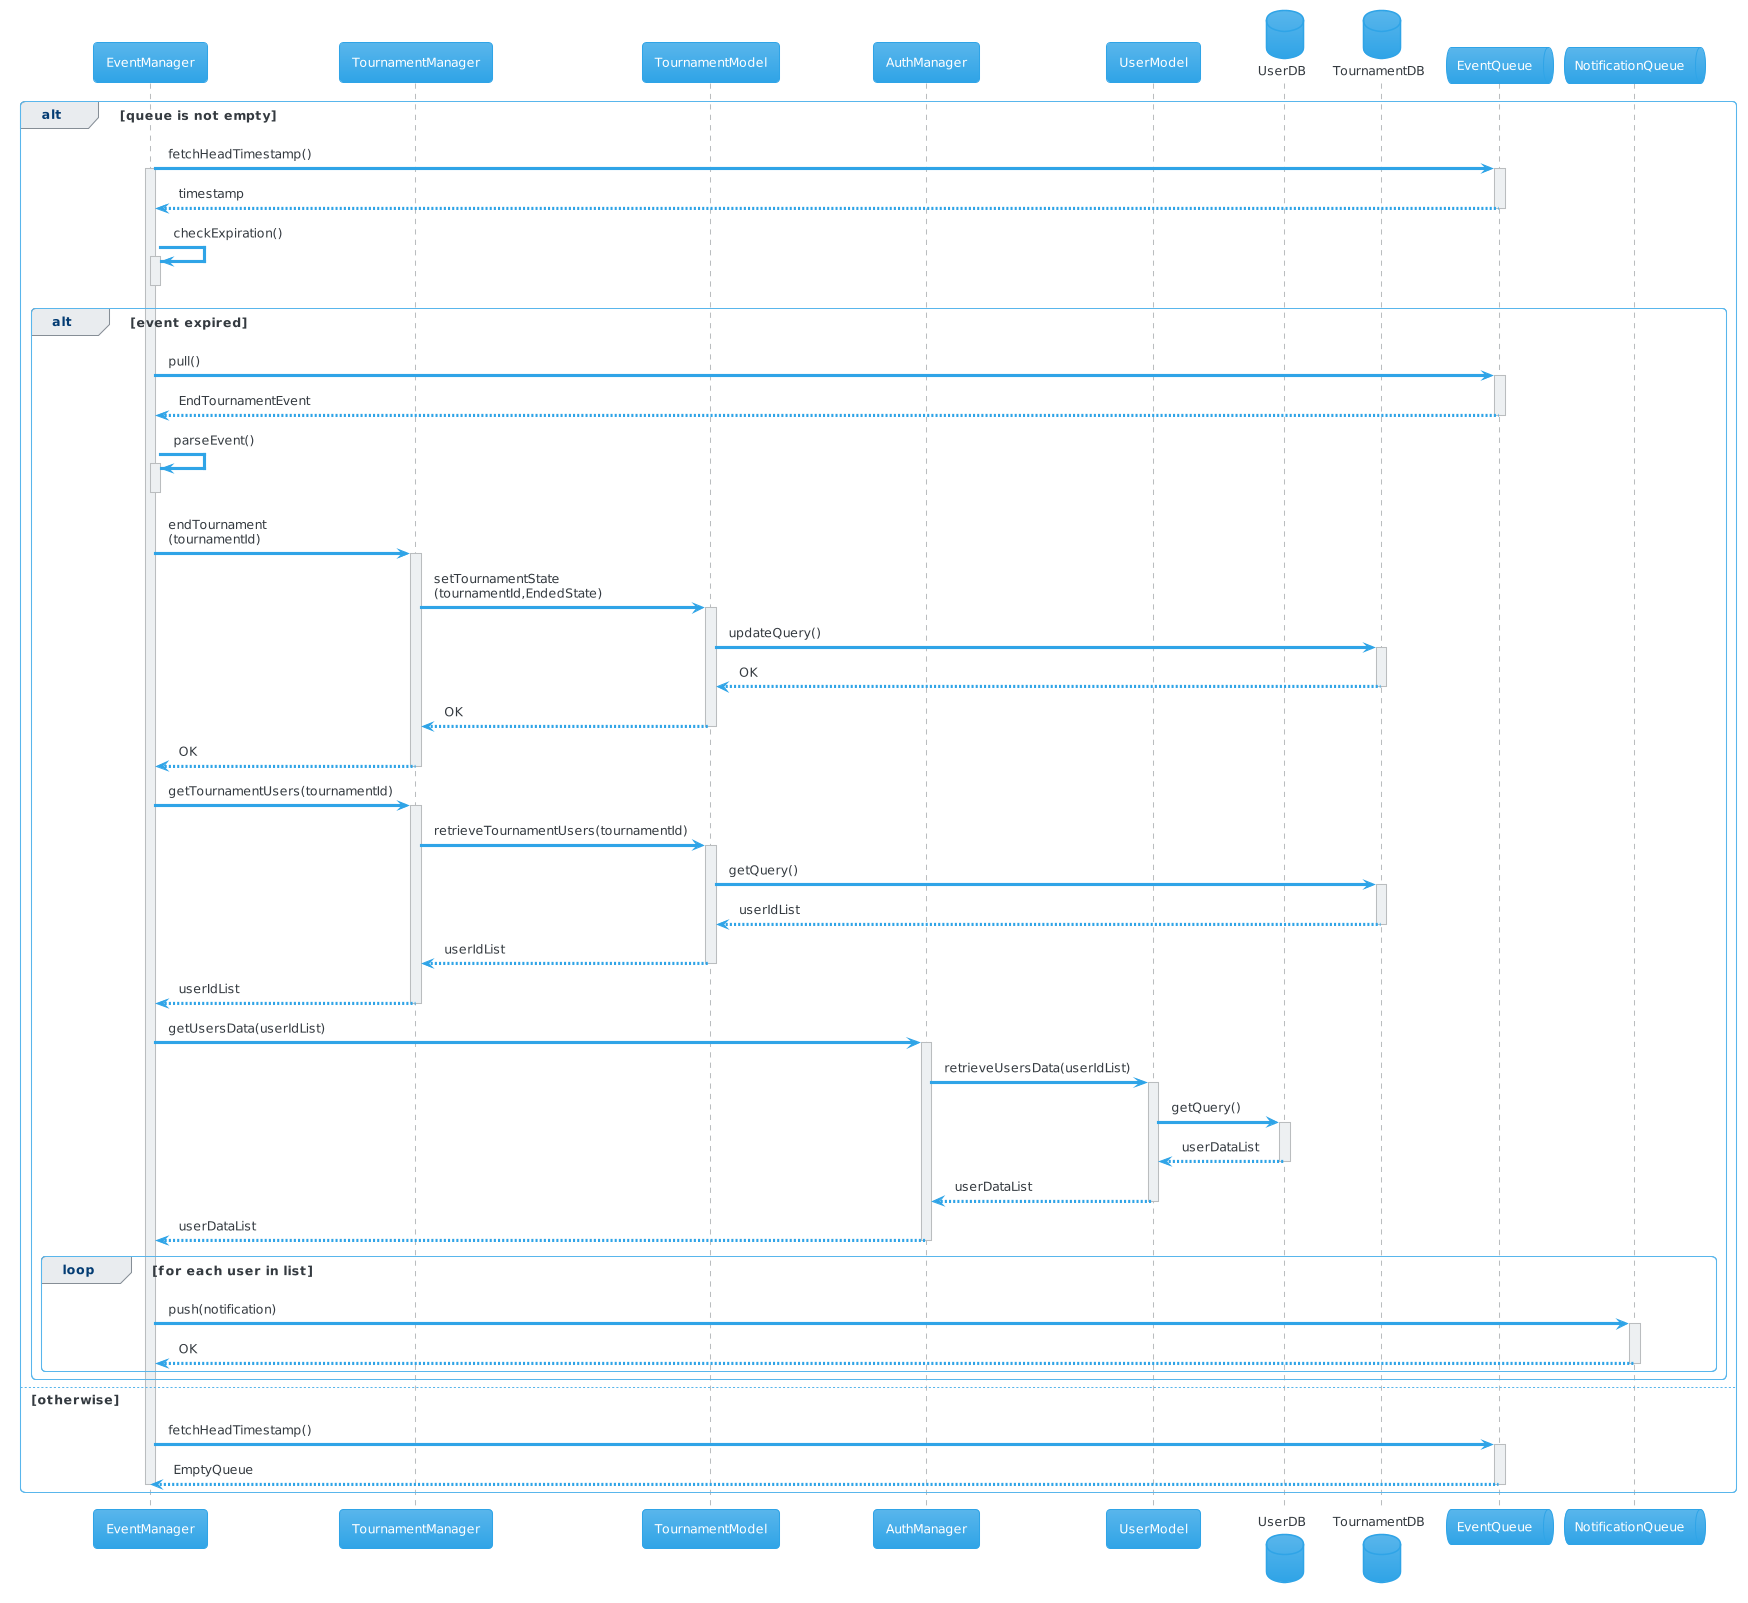
\includegraphics[width=1.2\textwidth]{Diagrams/sequence/close_tournament_pull.png}
    \caption{Pull of the notification event generated by the end of a tournament}
\end{figure}

\subsubsection{Pull of an email notification request}
\begin{figure}[H]
    \hspace{0.3cm}
    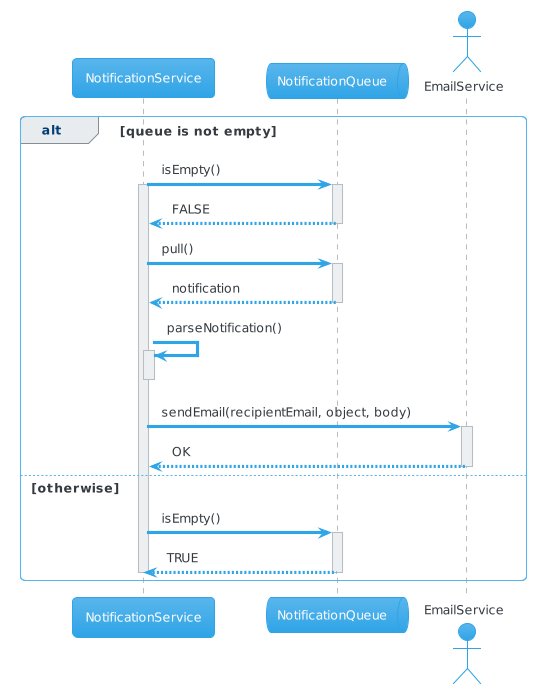
\includegraphics[width=0.9\textwidth]{Diagrams/sequence/pull_notification.png}
    \caption{Notification Service pulling a notification request and generating the relative email}
\end{figure}

\newpage
\subsection{Architectural styles and patterns}
\begin{itemize}
    \item \textbf{Client-Server}: the system can be seen as a client-server architecture from the point of view of the client, since it is composed of a front-end application (the client) and a back-end system (the server). The client is the web application that users interact with, while the server is the CKB Distributed System, which is constitued by multiple microservices. 
    The client and the server communicate over a network to perform specific tasks and to exchange data. The client sends requests to one of the available webserver instances, which in turn processes the request and replies with the appropriate response.
    The webserver, to process the request, redirects it to an API Gateway instance, which is the entry point of the backend system.
    \item \textbf{Microservices}: the back-end, as previously described, is composed of multiple microservices. This architectural style has been chosen because it allows to decompose the system into multiple almost-independent components, each one responsible for specific tasks.
    This is particularly useful in terms of deployment and scalability, since each node can be scaled independently from the others, which is fundamental in a system that is expected to handle a large variety of requests with different workloads.
    Concerning maintainability, this also allows to easily modify and update the system, since each microservice can be updated independently from the others.
    Also availability is improved, since the failure of a single microservice may not affect the availability of some functionalities of the system.
    \item \textbf{API gateway}: the API gateway pattern is similar to the facade pattern from object-oriented design, but it is part of a distributed system reverse proxy or gateway routing for using as a synchronous communication model.
    More in details, it acts as the system's facade, so it provides a single entry point to the APIs allowing the encapsulation of the underlying system architecture.
    It also works as a reverse proxy, since it route requests to internal microservices endpoints and is responsible of cross-cutting concerns such as load balancing, caching, security.
    \item \textbf{REST APIs}: the REST architectural style has been chosen to implement the communication between the client, the system and microservices, since it is the most common and widely used style for building web APIs.
    Additionally, REST APIs are stateless, which means that no client context is stored on the server between requests, simplifying implementation and horizontal scaling.. HTTPS is used as communication protocol and data exchanges are performed through JSON objects.
    \item \textbf{Model View Controller}: the MVC pattern decomposes the program logic into three interconnected elements:
    \begin{itemize}
        \item \textbf{Model}, which represents the dynamic data structure of the application, independent of the user interface. It is responsible for managing the data of the application and receives user input from the controller.
        \item \textbf{View}, which is responsible for the presentation of the data to the user. It sends user input to the controller.
        \item \textbf{Controller}, which is responsible for handling user requests and updating the model and the view accordingly. The state of the controller is inferred from the state of system which is represented by the model.
    \end{itemize}
    \item \textbf{Routing patterns}: the ServiceRegistry component enables the service discovery. Each microservice mantains a local cache of the registry, and periodically refreshes it by contacting the ServiceRegistry.
    Microservices use the local cache to contact other microservices and spread the load across the available instances following a round-robin schema.
    The ServiceRegistry is replicated through a master-slave schema, to ensure the availability of the service discovery functionality.
    \item \textbf{Security patterns}: the system uses the OAuth2 protocol to authenticate users. This protocol allows the system to delegate the authentication to an external identity provider. The system only receives a token from the identity provider, which is used to identify the user in the system.
    \item \textbf{Communication patterns}: both synchronous and asynchronous patterns are used in the system. The asynchronous communication pattern, which is implemented through the use of one-way queues, has been used for the communication between microservices that do not require any response from the receiver.
    This event-driven approach enforces the decoupling between microservices and concurs to the scalability of the system, since multiple instances of the same microservice can consume from the same queue and process the requests concurrently.
    The choice of a hybrid approach, is driven by the following advantages related to the synchronous communication:
    \begin{itemize}
        \item \textbf{Reduced latency}: synchronous requests allow services to retrieve data with minimal delay, providing fast response times. This is important for user-facing services like the API Gateway.
        \item \textbf{Simplicity}: does not require the use of queues and complex mechanism to handle bidierectional communication. This reduces complexity for services with simple integration needs.
        \item \textbf{Transactional integrity}:  allow several operations to be executed as an atomic transaction, ensuring data consistency across services. Useful when multiple services need to update related data.
        \item \textbf{Request-response pattern}: some use cases have an inherent request-response flow that fits synchronous communication. For example, the API Gateway may need to query other services to aggregate the response for the client.
    \end{itemize}

\end{itemize}
\subsection{Other design decisions}
In this section some other design decisions are presented and justified.
\begin{itemize}
    \item \textbf{Database solutions}: the database technologies and models have been chosen analyzing the most common interactions and queries that the system will perform. 
    A \textbf{document-oriented} database fits particularly well the TournamentDatabase, given the hierarchical structure of tournaments, battles and teams. The use of a unique tournament collection allows to perform useful and common queries without performing complex joins, which would be required in a relational database.
    Additionally, no drawbacks are expected in terms of redundancy, as no users data is stored in the TournamentDatabase (only the userIds are stored).
    However, \textbf{indexes} will be needed to quickly retrieve some data without performing a full scan of the collection, such as tournaments and battles data related to a specific user. These kind of indexes are indeed useful to populate the customized user's homepage or accessing battle or team data directly using their respective ids.
    A document-oriented database is also a good choice for the tournament collection, as it allows to conveniently store complex and unstructured data, such as tournament/battle scores and ranks within the same data structure.
    The UserDatabase instead is a \textbf{relational} database, since the data stored in it is structured and simple and no complex queries are expected to be performed on it.
    \item \textbf{Code Kata files}: as described in the RASD document, the educators are asked to provide some files to create a new battle. The system expects the project files to be correctly formatted, in order to be able to create the battle repository and to evaluate the submissions.
    The uploaded file must be a zip file containing the following:
    \begin{itemize}
        \item \textbf{src} folder containing the source code of the project, including build automation scripts (e.g. pom.xml for Maven projects, build.gradle for Gradle projects, make files for C projects and so on). 
        \item \textbf{test.txt} file containing the test cases to be used to evaluate the submissions. The file must contain one test case per line, and each test case must be formatted as follows:\\
         \textit{input1,input2,...,inputN;output}
    \end{itemize}
\end{itemize}

%personalized listings
\newcommand\YAMLcolonstyle{\color{black}\mdseries}
\newcommand\YAMLkeystyle{\color{black}\bfseries}
\newcommand\YAMLvaluestyle{\color{blue}\mdseries}
\newcommand\ProcessThreeDashes{\llap{\color{cyan}\mdseries-{-}-}}

It is now showed the structure of an example tournament document.\\

\lstdefinestyle{yaml}{
    basicstyle=\footnotesize\ttfamily,
    numbers=left,
    numberstyle=\tiny\color{gray},
    breaklines=true,
    showstringspaces=false,
    tabsize=2,
    frame=single,
    captionpos=b,
    keywords={true,false,null,y,n},
    sensitive=false,
    comment=[l]{\#},
    morecomment=[s]{/*}{*/},
    commentstyle=\color{red}\ttfamily,
    stringstyle=\YAMLvaluestyle\ttfamily,
    moredelim=[l][\color{orange}]{\&},
    moredelim=[l][\color{magenta}]{*},
    moredelim=**[il][\YAMLcolonstyle{:}\YAMLvaluestyle]{:},   % switch to value style at :
    morestring=[b]',
    morestring=[b]",
    literate =    {---}{{\ProcessThreeDashes}}3
                  {>}{{\textcolor{red}\textgreater}}1     
                  {|}{{\textcolor{red}\textbar}}1 
                  {\ -\ }{{\mdseries\ -\ }}3,
}
\lstinputlisting[style=yaml,caption={Your YAML Data},label={lst:yamlData}]{util/tournament.yaml}
